\documentclass[11pt]{article}
%\usepackage{illcmolthesis}
\usepackage{geometry}
\geometry{letterpaper} 
\usepackage{graphicx}
\usepackage{amssymb,amsmath}
\usepackage{bussproofs}
\usepackage[round, authoryear, comma]{natbib}
\usepackage{hyperref}
 \hypersetup{
     colorlinks,%
     citecolor=black,%
     filecolor=black,%
     linkcolor=black,%
     urlcolor=black
 }

\usepackage{gn-logic14}
\usepackage{subfigure}
\usepackage[geometry]{ifsym}

\usepackage{tabularx,booktabs,multirow}

%%%%%%%%%% TeXmacs macros
\newcommand{\assign}{:=}
\newcommand{\tmtextsf}[1]{{\sffamily{#1}}}
\newcommand{\tmem}[1]{{\em #1\/}}
\newcommand{\tmop}[1]{\ensuremath{\operatorname{#1}}}
\newcommand{\tmtextit}[1]{{\itshape{#1}}}
\newcommand{\tmstrong}[1]{{\textbf{#1}}}
\newcommand{\tmtextsc}[1]{{\scshape{#1}}}
\newcommand{\colons}{\,:\,}
\newcommand{\mathbbm}{\mathbb}

%%%%%%%%%% Enumitem Environments
\usepackage{enumitem}

\newlist{mynum}{enumerate}{10} 
\setlist[mynum]{label=\textup{(\emph{\arabic*})}, topsep=0.0in, parsep=0.00in}

\newlist{myRoman}{enumerate}{10} 
\setlist[myRoman]{label=\textup{(\emph{\Roman*})}, topsep=0.0in, parsep=0.075in}

\newlist{myroman}{enumerate}{10} 
\setlist[myroman]{label=\textup{(\emph{\roman*})}, topsep=0.0in, parsep=0.075in}

\newlist{enumerateroman}{enumerate}{10} 
\setlist[enumerateroman]{label=\textup{(\emph{\roman*})}, topsep=0.0in, parsep=0.075in}

\newlist{empt}{itemize}{10} 
\setlist[empt]{label*=, topsep=0.1in, parsep=0.075in}

\newlist{bul}{itemize}{10} 
\setlist[bul]{label=$\bullet$, topsep=0.0in,parsep=0.075in,}
\setlist[bul,2]{label=$\circ$, topsep=0.0in,parsep=0.075in,}
\setlist[bul,3]{label=$\diamond$, topsep=0.0in,parsep=0.075in,}

\newlist{itemizedot}{itemize}{10} 
\setlist[itemizedot]{label=$\bullet$, topsep=0.0in,parsep=0.075in,}
\setlist[itemizedot,2]{label=$\circ$, topsep=0.0in,parsep=0.075in,}
\setlist[itemizedot,3]{label=$\diamond$, topsep=0.0in,parsep=0.075in,}

\newlist{myalpha}{enumerate}{10} 
\setlist[myalpha]{label=(\emph{\alph*}), topsep=0.1in, parsep=0.1in}

\textwidth = 6.5 in
\textheight = 8.5 in
\oddsidemargin = 0.0 in
\evensidemargin = 0.0 in
\topmargin = 0.0 in
\headheight = 0.0 in
\headsep = 0.0 in
\parskip = 0.1in
\parindent = 0.0in

%%%%%%%% AMSTHM environments
\usepackage{amsthm}
\numberwithin{equation}{subsection}
\newtheorem{theorem}{Theorem}[subsection]
\newtheorem{prop}[theorem]{Proposition}
\newtheorem{proposition}[theorem]{Proposition}
\newtheorem{corollary}[theorem]{Corollary}
\newtheorem{mydef}[theorem]{Definition}
\newtheorem{definition}[theorem]{Definition}
\newtheorem{example}[theorem]{Example}
\newtheorem{lemma}[theorem]{Lemma}
\renewcommand{\qedsymbol}{\small QED}

%%%%%%% Symbols

% Yeah, I use a lot of crazy symbols, now that I reflect on this.
% Upon reflection, this section has evolved into quite a spectacular mess.

% We're gonna want to undefine and redefine stuff...
\def\my@undefine#1{\let#1=\undefined}%

% Load fakeMnSymbol
% 'cause some MnSymbols in this are awesome, but many kind of suck
% and after a little bit of searching, it looks like someone arleady
% solved this crazy problem...
\usepackage[]{fakeMnSymbol}
\DeclareSymbolFont{mnsymbolc}{U}{MnSymbolC}{m}{n}

% Here are the symbols it looks like I use from here:
\newcommand{\largepentagram}{\MNSlargepentagram}
\newcommand{\powerset}{\MNSpowerset}
\newcommand{\diamondminus}{\MNSdiamondminus}
\newcommand{\diamondplus}{\MNSdiamondplus}

% Sometimes, we are going to need more subtle hacks, so things can be
% in superscripts.  \MNSxxx symbols are in \mbox... fucking LaTeX...
\my@undefine{\boxminus}
\DeclareMathSymbol{\boxminus}      {2}{mnsymbolc}{112}
\my@undefine{\boxplus}
\DeclareMathSymbol{\boxplus}      {2}{mnsymbolc}{116}
\my@undefine{\Box}
\DeclareMathSymbol{\Box}      {2}{mnsymbolc}{106}
\renewcommand{\boxtimes}{\MNSboxtimes}
\newcommand{\boxslash}{\MNSboxslash}
\renewcommand{\Diamond}{\MNSmeddiamond}

% stdmaryrd has the best lightning symbol
\DeclareSymbolFont{stmry}{U}{stmry}{m}{n}
\SetSymbolFont{stmry}{bold}{U}{stmry}{b}{n}
\DeclareMathSymbol\lightning\mathord{stmry}{"20}

% Mathabx Font has cool corner symbols
\DeclareFontFamily{U}{matha}{\hyphenchar\font45}
\DeclareFontShape{U}{matha}{m}{n}{
      <5> <6> <7> <8> <9> <10> gen * matham
      <10.95> matham10 <12> <14.4> <17.28> <20.74> <24.88> matham12
      }{}
\DeclareSymbolFont{matha}{U}{matha}{m}{n}
\DeclareFontSubstitution{U}{matha}{m}{n}

\DeclareFontFamily{U}{mathb}{\hyphenchar\font45}
\DeclareFontShape{U}{mathb}{m}{n}{
      <5> <6> <7> <8> <9> <10> gen * mathbm
      <10.95> mathbm10 <12> <14.4> <17.28> <20.74> <24.88> mathbm12
      }{}
\DeclareSymbolFont{mathb}{U}{mathb}{m}{n}
\DeclareFontSubstitution{U}{mathb}{m}{n}

% I only use a few of these crazy mathabx symbols
\DeclareMathSymbol{\VDash}         {3}{mathb}{"28}
\DeclareMathSymbol{\DashV}         {3}{mathb}{"29}
\DeclareMathSymbol{\nVDash}        {3}{mathb}{"2A}
\DeclareMathSymbol{\nDashV}        {3}{mathb}{"2B}
\DeclareMathSymbol{\Vvdash}        {3}{mathb}{"2C}
\DeclareMathSymbol{\nVvdash}        {3}{mathb}{"2E}
\DeclareMathSymbol{\lcorners}      {4}{mathb}{"76}% name to be checked
\DeclareMathSymbol{\rcorners}      {5}{mathb}{"77}% name to be checked
\my@undefine{\ulcorner}%
\DeclareMathSymbol{\ulcorner}      {4}{mathb}{"78}% name to be checked
\my@undefine{\urcorner}%
\DeclareMathSymbol{\urcorner}      {5}{mathb}{"79}% name to be checked
\my@undefine{\llcorner}%
\DeclareMathSymbol{\llcorner}      {4}{mathb}{"7A}% name to be checked
\my@undefine{\lrcorner}%
\DeclareMathSymbol{\lrcorner}      {5}{mathb}{"7B}% name to be checked
\newcommand{\lc}{\ullcorner}
\newcommand{\rc}{\ulrcorner}

% For my EviL completeness symbol, I use upside down crosses... (I use pifont)
\newcommand{\Pifont}[1]{\fontfamily{#1}\fontencoding{U}%
                                           \fontseries{m}\fontshape{n}\selectfont}
\newcommand{\Pisymbol}[2]{{\Pifont{#1}\char#2}}
\newcommand{\ding}{\Pisymbol{pzd}}
\renewcommand{\Cross}{\textrm{\ding{61}}}
\newcommand{\iCross}{\mathrel{\reflectbox{\rotatebox[origin=c]{180}{\Cross}}}\!}
\newcommand{\invis}{\iCross}
\newcommand{\lhookrightarrow}{\hookrightarrow}
\newcommand{\nmodels}{\nvDash}
\renewcommand{\diamondsuit}{\Diamond}
\newcommand{\bs}{\ensuremath{\backslash}}
\newcommand{\evil}{\textsc{EviL} }
\newcommand{\Omegap}{\Omega}
\renewcommand{\Omega}{\mathfrak{M}}
\newcommand{\ra}{\rangle}
\newcommand{\la}{\langle}
\newcommand{\ipent}{\mathrel{\reflectbox{\rotatebox[origin=c]{180}{\ensuremath{\largepentagram}}}}\!\!\!}
\newcommand{\ang}{\Lambda}
\newcommand{\DD}{\diamondminus}
\newcommand{\DDI}{\diamondplus}
\newcommand{\pDD}{\diamondslash}
\newcommand{\pDDI}{\diamondtimes}
\newcommand{\Nec}{\Box}
\newcommand{\Pos}{\Diamond}
\newcommand{\BD}{\boxdot}
\newcommand{\BM}{\boxminus}
\newcommand{\DM}{\diamondminus}
\newcommand{\PD}{\diamonddot}
\newcommand{\BP}{\boxplus}
\newcommand{\nin}{\not\in}
\newcommand{\BB}{\boxminus}
\newcommand{\pBB}{\boxslash}
\newcommand{\BBI}{\boxplus}
\newcommand{\pBBI}{\boxtimes}
\newcommand{\NM}{\boxminus}
\newcommand{\PP}{\circlearrowleft}
\newcommand{\DP}{\diamondplus}
\newcommand{\PM}{\diamondminus}
\newcommand{\falsum}{\bot}
\newcommand{\FB}{\filledmedsquare}
\newcommand{\BlackBox}{\filledmedsquare}
\newcommand{\NT}{\boxtimes}
\newcommand{\PT}{\diamondtimes}
\newcommand{\INP}{\boxplusI}
\newcommand{\INM}{\boxminusI}
\newcommand{\mo}[2]{\ensuremath{\mathfrak{M},( #1, #2 )}}
\newcommand{\pr}[2]{\ensuremath{( #1, #2 )}}
\newcommand{\rel}[1]{\ensuremath{R_{#1}}}
\newcommand{\kl}{\theta}
\usepackage{tikz}
\usetikzlibrary{arrows}


\title{Evidentialist Logic}
\author{Matthew P. Wampler-Doty}
%\birthdate{May 23rd, 1984}
%\birthdate{}
%\birthplace{Boston, Massachusetts, USA}
%\birthplace{}
%\defensedate{}
%\supervisor{Prof.dr J. F. A. K. van Benthem}
\date{}

\begin{document}
\maketitle
\pagebreak
\tableofcontents
\pagebreak


\section{Philosophy}\label{philosophy}
\subsection{Forward}
The idea of applying modal logic to the study of knowledge more or
less began with \citet{hintikka_knowledge_1969}.  In this it is
suggested that one can use the possible world framework of modal logic
to model ideal logical agents, and reason about concepts like
knowledge and belief as modal $\Box$s.  In Hintikka's original text,
some philosophical emphasis is put on the ideas of
\emph{introspection}, which have two formulations:
\begin{bul}
	\item Positive: $\Box \phi \to \Box\Box \phi$ - ``If the agent knows a fact, then she knows that she knows this.''
	\item Negative: $\Pos \phi \to \Box\Pos \phi$ - ``If the agent does not know a fact, she knows that she does not know this.''
\end{bul}
Intuitively, the second idea seems like something one ought to reject
outright.  Many will recall the somewhat famous piece of sophistry put
forward by former US secretary of defense Donald Rumsfeld
\citep{rumsfeld_defense.gov_2002}:
\begin{quote}
Reports that say that something hasn't happened are always interesting
to me, because as we know, there are known knowns; there are things we
know we know. We also know there are known unknowns; that is to say we
know there are some things we do not know. But there are also unknown
unknowns -- the ones we don't know we don't know. And if one looks
throughout the history of our country and other free countries, it is
the latter category that tend to be the difficult ones.\end{quote}

This quote was ultimately part of a larger, more diabolical
justification for criminal military action.  Still, it is undeniably
at variance with negative introspection; and despite its malicious
intent behind it, it is compelling.  Furthermore, Hintikka also
rejects negative introspection; and while it would seem from the above
quote that Rumsfeld does not reject positive introspection, Hintikka
does so explicitly \citep{hintikka_knowledge_1969}.

Despite philosophical objections, the received view in modern
epistemic logic embraces both negative and positive introspection.  In
addition, the following axiom is also considered:
\begin{bul}
	\item Reflection: $\Box \phi \to \phi$ - ``If the agent knows a some statement, that statement is true''
\end{bul}
These three axioms together, along with the axioms and rules of elementary modal logic, form C.I. Lewis' system $S5$ \citep{lewis_symbolic_1951}.  Under correspondence theory, these axioms express that the underlying accessibility modal relation is an equivalence relation. That is, they express that the ideal agent under investigation has partitioned their state space into \emph{information states}.  It is well known that game theory shares an equivalent notion of information states (see, for instance, \citet{halpern_set-theoretic_1999} and \citet[chapter 3]{rubinstein_modeling_1998}).

And while this view of knowledge finds industrial application, such as
in \citet{agray_ban_2002} and
\citet{hommersom_toward_2005,hommersom_update_2004}, it presents an
perspective on knowledge which is not very human.\footnote{Admittedly,
  most of the criticisms I shall levy against mainstream epistemic
  logic in the subsequent discussion are known to the
  epistemic logic community.  I understand it is preferred that they
  be swept under the carpet and never mentioned, as they are fairly painful
  to remember for epistemic logic enthusiasts. I am not particularly
  apologetic in recounting the basic failures of epistemic logic as an 
  intellectual exercise.  The discussion I present in this section is
  intended for people new to epistemic logic, who may be unaware of
  its basic inadequacies and irrelevance.}


\subsection{Thermometers}\label{thermometers}
Imagine a 1 m$^3$ box with a thermometer sealed hermetically inside, as in Fig.  \ref{fig:therm1}.  Further, pretend that the thermometer reads 290 Kelvin.  How many moles of gas are in the chamber?

\begin{figure}[ht]
\begin{center}
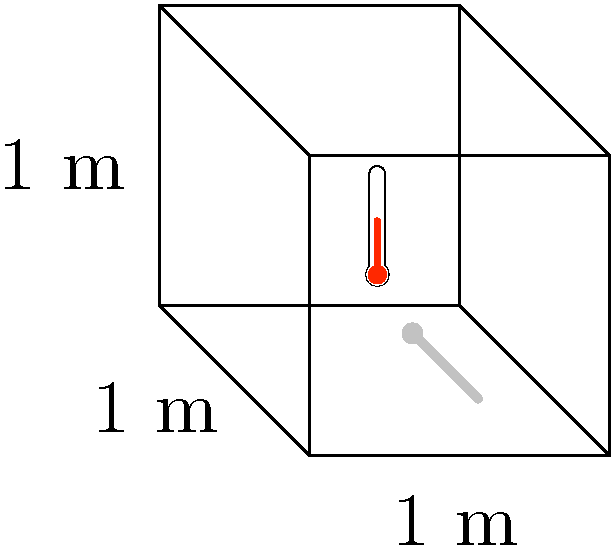
\includegraphics[scale=.5]{thermometer.pdf}
\end{center}
\caption{A thermometer in a box}
\label{fig:therm1}
\end{figure}

The answer is indeterminate.  Recall that the the \emph{ideal gas law} was originally discovered by \'{E}mile Clapeyon \citep{clapeyron_mmoire_1834}; in modern parlance it reads:
\[ P V = n R T\]
Where:
\begin{bul}
\item $P$ is the pressure in pascals
\item $V$ is the volume in cubic meters
\item $n$ is the number of moles of gas
\item $T$ is the temperature in Kelvins
\item $R$ is the \emph{ideal gas constant}, $\approx8.3$ J$\cdot$K$^{-1}\cdot$mol$^{-1}$
\end{bul}

With the ideal gas law, we can see that the thermometer is effectively in an epistemic space.  To be explicit, consider the basic modal language with the following grammar:
\[ \phi ::= x \textup{ pascals}  \ |\ y \textup{ moles}  \ |\ z \textup{ Kelvin}  \ |\ \phi \to \psi \ |\ \bot \ |\ \Box \phi \]

This can be seen to be an ordinary modal language with three kinds of letters.  Under this language, we can naturally understand that the thermometer is an epistemic agent in an $S5$ model for this language.  Explicitly, the model is the triple $\langle W, V, \sim \rangle$ where:
\begin{bul}
	\item $W$ is pairs $(P,n)$ where $P$ is some positive pressure in pascals and $n$ is some positive number of moles.
	\item $V$ is defined as follows:
	\begin{bul}
		\item $(P,n) \in V(x \textup{\ pascals})$ if $P = x$
		\item $(P,n) \in V(y \textup{\ moles})$ if $n = y$
		\item $(P,n) \in V(z \textup{\ Kelvin})$ if $z = \frac{P}{n \cdot R}$
	\end{bul}
	\item Finally, $(P,n) \sim (P',n')$ holds if and only if $P \cdot n' = P' \cdot n$ 
\end{bul}
We can also visualize the information states in Fig.  \ref{fig:therm2}; they form rays emanating from the origin.

Now, I give this example because it is representative of the perspective provided by epistemic logic - agents are essentially elaborate \emph{sensor networks} in the received view.  Imagine we were to go up to an agent and ask her why she believes some proposition $\phi$; what could she possibly say?  She'd say she feels $\phi$ with every fiber of her being, that it's true in every conceivable world she can think of.  The reason that $\phi$ occurs to the agent is because it's what her sensory instruments tell her. Methodologically, this is exactly the same as the way the thermometer was modeled in the previous thought experiment. To this end I shall abbreviate the received view on epistemic logic as the \emph{thermometer theory of knowledge}.

This isn't knowledge.  The thermometer theory is inadequate:  if I were to ask a person why she believes a proposition $\phi$, I probably wouldn't accept appeals that she cannot conceive of the contrary as possible.  I'd want some kind of explanation, especially if $\phi$ were a piece of mathematics, to give principle example.  It would certainly make the enterprise of mathematics far simpler if proving theorems amounted to exhibiting that their negation is not imaginable.  This gives rise to the following philosophical observation:
\begin{quote}
\textbf{Thermometer Principle}: \emph{Traditional epistemic agents, like thermometers, don't really have knowledge, since one must have reasons for the things they believe.}
\end{quote}

As I will elaborate, the above assertion follows from more general concerns I have with epistemic logic.

\begin{figure}[ht]
\begin{center}
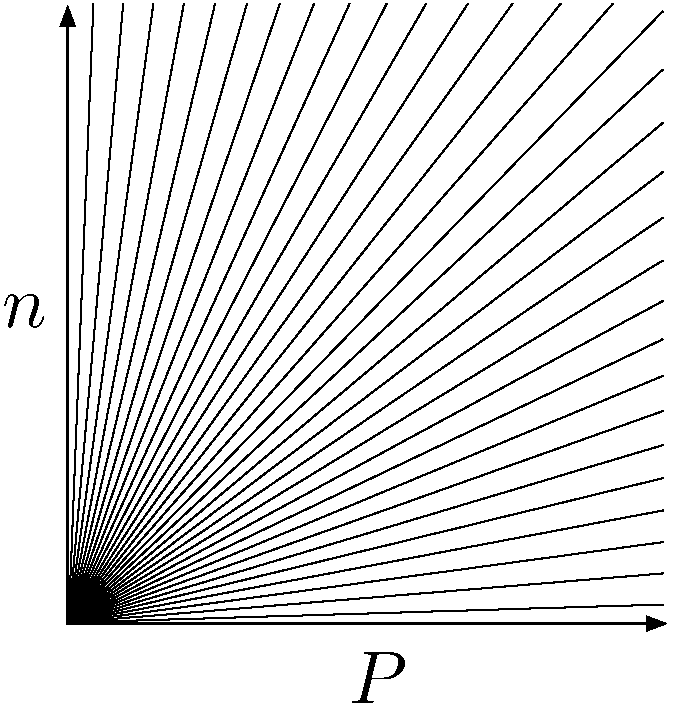
\includegraphics[scale=.5]{therm.pdf} 
\end{center}
\caption{Thermometer information states}
\label{fig:therm2}
\end{figure}
\subsection{Explicit Justification}\label{explicit}

I hold that the \emph{Thermometer Principle} is an expression of the following more fundamental idea:
\begin{quote}
 \textbf{Justification Principle}: \emph{In order to know something, one must have a some kind of sufficient justification.}
\end{quote}
I contend that derivation in a logical calculus is suitable
justification for the above principle. In light of this, all of my
future developments shall center around the idea that in order to have
knowledge, one must have a special derivation.  Since knowledge
entails belief \citep[under the traditional view in]{gettier_is_1963},
I have decided to simply equate belief with having a derivation.
Hence knowledge can then be thought of a species of this kind of
derivational belief. And while it is perhaps as bad an
oversimplification as the thermometer view I have previously
criticized, my modeling technique assumes \emph{doxastic omniscience},
which is to say that I assume an agent's beliefs are closed under
logical consequence\footnote{\cite{hintikka_knowledge_1969} assumes a
  similar perspective; for modeling purposes, the agent is assumed to
  have adequate time to realize the consequences of their beliefs.
  Similarly, we might interpret belief as what is refered to in
  \citet{levesque_logic_1984} as ``implicit belief.''}.  This will be illustrated shortly.

The \emph{Justification Principle} is similar to demanding
\emph{explicit justification} for beliefs in epistemic logic. I am not
the first person to suggest this. The modern hunt for logics of
explicit justification appears to have been initiated in
\citet{van_benthem_reflectionsepistemic_1991}\footnote{While this
  paper is considered seminal, it should be remarked that research
  into this subject began prior to it.  Specifically, the
  \emph{phrase} ``explicit belief'' appears to have its origins in
  \citep{levesque_logic_1984}.}. One framework which has been proposed
to achieve this is \emph{Justification Logic}
\citep{artemov_introducing_2005,artemov_justification_2007,fitting_logic_2004,fitting_logic_2005}.
Alternative frameworks for reasoning about implicit/explicit
information have also been proposed in \citet{van_benthem_inference_2009} and
\citet{velzquez-quesada_inference_2009}.


\subsection{Sketch}\label{sketch}

These analyses mentioned in the previous section are all quite
sophisticated; I have in mind something comparatively na\"{i}ve.  
I shall present a sketch in this section -- that being said I intend
to be extremely informal.  A formal development of the ideas shall be 
given in \S\ref{evil-grammar}.  With this proviso, consider the basic
modal language $\mathcal{L}(\Phi)$:
\[ \phi ::= p \in \Phi \ |\ \phi \to \psi \ | \ \bot \ |\ \Box \phi \]

Further, let $\Omega \subseteq \powerset \Phi \times \powerset \mathcal{L}(\Phi)$, that is, let $\Omega$ be pairs of sets of letters and formulae. Define the following truth predicate $\VDash$ recursively as follows:
\begin{empt}
 \item $\Omega, (a,A) \VDash p \iff p \in a$
 \item $\Omega, (a,A) \VDash \phi \to \psi \iff \Omega, (a,A) \VDash \phi$ implies $\Omega, (a,A) \VDash \psi$
 \item $\Omega, (a,A) \VDash \bot \iff False$
 \item $\Omega, (a,A) \VDash \Box \phi \iff $ for all $(b,B) \in \Omega$, $\Omega,(b,B) \VDash A$ implies $\Omega, (b,B)\VDash \phi$ for all $(b,B) \in \Omega$
\end{empt}

Since the semantics like the above shall be the principle objects of
study, I will give how I read them philosophically.  In these
semantics, instead of thinking of every world individually, I think of
every world as containing facts and a part of the agent's mind.  This
part of the agent's mind is represented by what I shall refer to as
propositions which she ascents to. I shall refer to these
interchangeably as \emph{premises}, \emph{assumptions}, \emph{basic
  beliefs}, \emph{experiences} or \emph{evidence}.  On the basis of
her evidence, I imagine the agent composes arguments using the logic
of semantics suggested and all of the worlds that are possible.  In
this way, I consider this approach to be roughly in line with the
\emph{evidentialist} view on epistemology, which
\citet{conee_evidentialism_2004} describe as follows:
\begin{quote}
  [E]videntialism is a supervenience thesis according to which facts
  about whether or not a person is justified in believing a
  proposition supervene on facts describing the evidence that the
  person has.
\end{quote}
$\ldots$however, while my sympathies are with this perspective on
epistemology, they differ foundationally - while evidentialism
develops intuitions using analytical philosophy, our approach shall be
founded in formal semantics like the one above.

That is, if a proper foundation can be provided at all.  Admittedly,
the above formulation of truth immediately runs into a \emph{paradox}
- for instance, if 
\begin{bul}
\item $a:=\varnothing$ 
\item $A:=\{\Box \bot\}$
\item and $\Omega:= \{(a,A)\}$
\end{bul}
\ldots then $\Omega,(a,A)\VDash \Box \bot$ has an indeterminate truth
value.  So let $\mathcal{L}_0(\Phi)$ be the propositional fragment of
$\mathcal{L}$; we shall restrict the truth value to $\Omega\subseteq
\Phi \times \powerset \mathcal{L}_0(\Phi)$.  This suffices to make
every truth value of this logic determinate.

We may observe that the logic of these semantics is familiar:
\begin{prop}
Assuming that the set of proposition letters $\Phi$ is infinite
$$\vdash_{K} \phi\textup{ if and only if } \Omega, (a,A) \VDash \phi \textup{ for all finite $\Omega$ for all $(a,A) \in \Omega$}$$
\ldots where $K$ is basic modal logic.
\end{prop}
\begin{proof}
 Left to right is trivial, so we shall focus on right to left.  Assume
 that $\nvdash_{K} \phi$, then we know from completeness and the
 finite model property that there's some finite model
 $\mathbb{M}=\langle W^\mathbb{M}, V^\mathbb{M}, R^\mathbb{M}\rangle$ and world $w \in W^\mathbb{M}$ such that $\mathbb{M},w \nVdash \phi$ (see \citet[chapters 2 \& 4]{blackburn_modal_2001} for details of these facts).

Now let $\Lambda_\phi$ be the proposition letters that occur as
subformulae of $\phi$, and let $\rho_\phi : W^\mathbb{M} \hookrightarrow \Phi \bs \Lambda_\phi$ be an injection.  Define $\theta_\phi:W^\mathbb{M}\to \powerset\Phi \times \powerset \mathcal{L}_0(\Phi)$ as follows\footnote{I am indebted to Johan van Benthem for the invention of this particular function.}
\begin{center}
\begin{minipage}{3in}
\begin{tabbing}
	$\theta_\phi(w) := ($ \= $\{p\in \Phi \ |\ \mathbb{M},w\VDash p\} \cup \{\rho_\phi(w)\},$\\
                       \> $\{ \bigvee \{\rho_\phi(v) \ | \ v\in W^\mathbb{M} \wedge w R^\mathbb{M}v \} \})$
\end{tabbing}
\end{minipage}
\end{center}

Now let $\Theta := \theta[W^\mathbb{M}]$. An induction on the complexity of subformulae $\psi$ of $\phi$ shows that 
$\mathbb{M},w\Vdash \psi \iff \Theta,\theta(w) \VDash \psi$ for all $w \in W^\mathbb{M}$.  Since 
$\mathbb{M}, w \nVdash \phi$ then we know that $\Theta,\theta(w)\nVDash \phi$, which completes the proof.
\end{proof}

Armed with this, we can see that these semantics are adequate for modeling agents according to my declared intentions, since we have the following:
\begin{prop}\label{central-prop}
 Let $A$ be finite and define $$Th(\Omega) := \{ \phi \in \mathcal{L}(\Phi) \ |\ \Omega, (a,A) \VDash \phi \textup{ for all $(a,A) \in \Omega$\}}$$
\ldots then $\Omega, (a,A) \VDash \Box \phi$ if and only if $Th(\Omega) \cup A \vdash_K \phi$.
\end{prop}
\begin{proof}
 To see left to right, just note that since $A$ is finite then if $\Omega, (a,A) \VDash \Box \phi$ evidently for all $(b,B)\in \Omega$ we have $\Omega, (b,B) \VDash \bigwedge A \to \phi$, which just means that $Th(\Omega) \cup A \vdash_K \phi$ by the deduction rule.

On the other hand if $Th(\Omega) \cup A \vdash_K \phi$, then we know that $Th(\Omega) \vdash_K \bigwedge A \to \phi$, and since $Th(\Omega)$ is sound for $\Omega$ we then have that for all $(b,B) \in \Omega$ that $\Omega,(b,B)\VDash \bigwedge A \to \phi$.  Since $A$ is finite we know that  $\Omega,(b,B) \VDash A$ if and only if $\Omega,(b,B) \VDash \bigwedge A$, and thus we can deduce that $\Omega,(a,A)\VDash \Box \phi$ by definition.
\end{proof}

A natural way to read $Th(\Omega)$ is the background knowledge the agent has about the universe she lives in.  This approach presents an analysis of modal logic whereby an idealized agent is modeled as closed under deduction; this is the \emph{doxastic omniscience} I have mentioned earlier. Under this view, evidently the agent's beliefs correspond to those things for which she has proofs.  This shall be the basis of my future investigations.

\subsection{The Human Condition}\label{Human-Condition}
To supplement to this basic framework, I shall try to illustrate how
further inspiration and desiderata can be drawn from the philosophical
literature.  It should be remarked that I do this in stark contrast to
the received view in epistemic logic
\citep[pg. 34]{lenzen_recent_1978}:
\begin{quote}
The search for the correct analysis of knowledge, while certainly of
extreme importance and interest to epistemology, seems not
significantly to affect the object of epistemic logic, the question of
the validity of certain epistemic-logical principles.
\end{quote}
\ldots quite to the contrary, I feel epistemic logic should not turn
it's back on philosophy. Philosophy critically provides guidance for
the intuitions behind how knowledge should be correctly modeled.  It
also provides a solid grounding in a proper treatment of knowledge.
However, engaging with philosophy is evidently not the thrust of
mainstream epistemic logic.

Most mainstream epistemic logic, the object of study is really the
nature of information, not human knowledge.  It applies equally well
to robots, \emph{homo economicus}, or thermometers as suggested in
\ref{thermometers}.  It's inspiration is not really in what it's like
to be a living person; it's more naturally based in artificial intelligence, automata
theory, algebra, topology, and other abstract disciplines.

In contrast, I propose the following principle:
\begin{quote}
 \textbf{The Human Condition}: \emph{The analysis of knowledge should strive for a basis in human experience}
\end{quote}
\ldots this principle indeed underpins the Justification Principle
provided in \S\ref{explicit}. This is because I feel that the belief
in a proposition can be thought of human only if the agent has a
reason associated with it.  Otherwise, it seems that in the absence of
reason, no account can be given for how the belief came about other
than through instrumentation, which is the thermometer view.

Embracing this principle, I shall turn to the development of my
thoughts from their philosophical origins.

\subsection{Soundness}\label{soundness}
So to give a shallow example of a basic application of a philosophical
idea, it is natural to insist that if knowledge is based on beliefs
generated via deduction from some set of premises, then those premises
have to be \emph{sound}. I suggest this can be done by introducing a
new operator $\circlearrowleft$ with the following semantics:
\[ \Omega,(a,A)\VDash \circlearrowleft \iff \Omega,(a,A)\VDash A\]
Armed with these semantics, a first guess at what constitutes
knowledge suggests it might be nothing more than possession of a
belief based on a sound set of premises. So a first approximation of
knowledge might be equated with the formula:
$$\circlearrowleft \wedge \Box \phi.$$
But is this anything like an adequate analysis of knowledge?

\textbf{No}. To illustrate why I shall resort to a thought experiment to motivate why I think to the contrary.
Imagine that Charlotte suspects, correctly, that if John has tried to murder
on Alex, then Alex has survived.  She further learns, correctly, that John
has indeed tried to murder Alex.  But later, she ``learns'' some erroneous
information asserting Vietnam is south of Malaysia.  If we codify all of this as
a set $C$, and let the real world be
denoted $c$ and the universe $\Omega$, evidently we have $\Omega, (c, C) \nVDash
\circlearrowleft$, so this previous definition of knowledge fails.  But
should it?  I don't think so; Charlotte's knowledge about John's unspeakable
betrayal of Alex is correct, as well as her inference that Alex is tough as
nails.  Just because she has been deluded regarding irrelevant facts
about geography shouldn't have any bearing on her
knowledge about Alex.
\subsection{Descartes}\label{Descartes}
In reflection on the previous section, it should be remarked that
philosophers have historically been concerned with defeasible
experiential data, going back at least as early as Plato's \emph{The
  Republic VII} \citep{jowett_republic_1998}.
In answer to the problem faced by the above analysis of knowledge, I
think guidance can be found in Descartes' \emph{Meditations}
\citep{vietch_descartes_2005}.  In
\tmtextit{Meditations I}, Descartes suggests that he might be in an enlightenment era
version of \tmtextit{The Matrix} created by an all powerful demon.  In
\tmtextit{Meditations II}, he famously suggests how one might escape this
trap:
\begin{quote}
{The Meditation of yesterday has filled my mind with so many doubts,
that it is no longer in my power to forget them. Nor do I see, meanwhile, any
principle on which they can be resolved; and, just as if I had fallen all of a
sudden into very deep water, I am so greatly disconcerted as to be unable
either to plant my feet firmly on the bottom or sustain myself by swimming on
the surface. I will, nevertheless, make an effort, and try anew the same path
on which I had entered yesterday, that is, proceed by casting aside all that
admits of the slightest doubt, not less than if I had discovered it to be
absolutely false; and I will continue always in this track until I shall find
something that is certain, or at least, if I can do nothing more, until I
shall know with certainty that there is nothing certain.}\end{quote}

This tactic proposes a natural solution to the problem the previous
thought experiment: \tmtextit{Charlotte can know that Alex survives if she
 argues {\tmstrong{only}} from her experience involving Alex and John.
 }  If like Descartes she can forget some of what she has come to believe that's a
little suspicious, she might be able to compose an argument with a sound basis that Alex is alive.
 Taking Descartes as inspiration, I would suggest a new semantic operation:
\[ \Omega,(a,A) \VDash \BM \phi 
     \iff \textup{ for all }(b,B)\in \Omega
           \textup{ such that }a = b
                   \textup{ and }B \subseteq A
            \textup{ then }\Omega,(b,B) \VDash \phi \]
This mechanism lets Charlotte access subsets of her beliefs, which
would then form the basis for various arguments she might compose.
Provided that $(c,C')\in \Omega$, where $C'$ is the same as $C$ but
doesn't mention erroneous beliefs about geographical data, it might
serve as a basis for Charlotte's knowledge that Alex survives.  This
suggests that the following equation might reasonably express a more
adequate notion of knowledge:
\[ \DM(\PP \wedge \Nec \phi) \]

\subsection{Contradictions}\label{contradictions}

There's hidden virtue in the previous analysis.  To see what it is, I
am inspired by the 19th century philosopher Ralph Waldo Emerson, who
writes in his essay \emph{Self-Reliance} \citep{emerson_essays_2008}:
\begin{quote}
{ Why drag about this corpse of your memory, lest you contradict
  somewhat you have stated in this or that public place? Suppose you
  should contradict yourself; what then? It seems to be a rule of
  wisdom never to rely on your memory alone, scarcely even in acts of
  pure memory, but to bring the past for judgment into the
  thousand-eyed present, and live ever in a new day. \ldots}

{A foolish consistency is the hobgoblin of little minds, adored by
  little statesmen and philosophers and divines. With consistency a
  great soul has simply nothing to do. He may as well concern himself
  with his shadow on the wall. Speak what you think now in hard words
  and to-morrow speak what to-morrow thinks in hard words again, 
though it contradict every thing you said to-day. 
-- `Ah, so you shall be sure to be misunderstood.' -- Is it so bad
then to be misunderstood? }
\end{quote}

A healthy lack of consistency is just part of what makes up the day to
day life of any living, sane person.
Isn't error-prone reasoning a hallmark of human thought?  And if a
love sick epistemic agent $\exists$ is getting mixed signals from
another epistemic agent $\forall$, why can't she draw inconsistent
conclusions about $\forall$'s feelings on the one hand, but still have
basic knowledge that $734\times 12 = 8808$ and other such irrelevant
facts?  I don't see why not.  Under these considerations, I'd embrace
the following:
\begin{quote}
 \textbf{Emerson's Principle}: \emph{One can be inconsistent and still have knowledge}
\end{quote}
Permit me illustrate how the framework I have given accommodates
this. My treatment is further inspired by a friend and contemporary of
Emerson's, the poet \emph{Walt Whitman}. In \emph{Leaves of Grass}
\citep{whitman_leaves_2008}, he writes:
\begin{center}{  Do I contradict myself?\\
  Very well then I contradict myself,\\
  (I am large, I contain multitudes.)}
\end{center}
So consider the model $\Omega$ in Fig. \ref{fig:example1}; this is
intended to be a toy model of how I interpret Walt Whitman in the
above stanza. This figure should be read as follows:
\begin{bul}
 \item if one point $(a,A)$ is above another point $(b,B)$ and
   connected by a densely dotted line 
   \tikz \draw[densely dotted,semithick](0pt,0pt) -- (20pt,6pt);, 
   this means that $a = b$ and $B \subset A$.
  \item if one point $(a,A)$ is connected to another point $(b,B)$ by
    a line with an arrow \tikz \draw[->,>=latex,semithick](0pt,0pt) --
    (20pt,6pt);, this means that $\Omega,(b,B) \VDash A$
\end{bul}
\begin{figure}[ht]
\begin{center}
  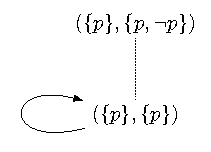
\includegraphics[]{example1/example1.pdf}
\end{center}
%
%\caption{Inconsistent, yet still has knowledge (contains multitudes)}
\caption{Inconsistent, yet still has knowledge}
\label{fig:example1}
\end{figure}
Observe that $\Omega,(\{p\},\{p,\neg p\}) \VDash \Box \bot$; it's
obvious that in this state Walt is being inconsistent since he clearly
believes contradictory things.  Simultaneously, we have that
$\Omega,(\{p\},\{p,\neg p\}) \VDash \DM (\PP \wedge \Box p)$; so we
figure that Walt has a sound argument that $p$.  Walt might be
inconsistent, but it would appear that \emph{at least one} of his
arguments makes sense.  And this is naturally because Walt contains a
multiplicity of inner selves, just like he says, which the the $\BM$
modality gives access to.

\subsection{Irrationality}\label{irrational}

Embracing contradiction runs contrary to the received view on
epistemic logic.  For instance, \citet{hendricks_wheresbridge?_2006}
write:
\begin{quote}
{ Epistemic logic does carry epistemological significance
 but in an inevitably idealized sort of way: One restricts attention to a
class of rational agents where rationality is defined by certain
postulates. Thus, agents have to satisfy at least some minimal
conditions to simply qualify as rational. This is by and large
what Lemmon originally suggests \citep{lemmon_symposium:_1959}.}
\end{quote}
Furthermore, it is conventional to think that rational agents do not
hold contradictions.\footnote{It should be remarked that
  \citet{priest_doubt_2006} explicitly rejects this perspective on
  rationality.  Priest points out that in times of scientific
  revolution, rational people naturally hold contradictory views. He
  suggests that a paraconsistent logic framework could account for a
  rational agent holding contradictory beliefs.  I profess sympathy
  for Priest's perspective; however, I am confident that this does not
  represent the received view which I am arguing against.}  For
instance, in \citep{kraus_knowledge_1986}, $\neg \Box \bot$ is taken
as an axiom (it is A9 in their numbering).

This is similar to the thermometer concept of knowledge we provided in
\S\ref{explicit}, since like the thermometer view, it's incompatible
with a human perspective.  Hence I extend the following:
\begin{quote}
 \textbf{Irrationality Principle}: \emph{Since humans are not
   rational, views on epistemic logic that postulate this should be
   rejected}
\end{quote}
I should mention that while this perspective is not typically embraced
in epistemic logic\footnote{Noted exceptions to this are
  \citet{rantala_impossible_1982} and \citet{levesque_logic_1984}.},
it finds sympathy in other logical traditions, namely in
\emph{relevance logic} and \emph{paraconsistent logic}, as already
noted \citep[see][chapters 1 \& 4]{gabbay_handbook_2002}.

Apart from inconsistency, I do not really accommodate very much
irrationality; I will freely admit that frameworks like
\citep{rantala_impossible_1982} and and \citet{levesque_logic_1984}
employing \emph{impossible world} semantics are far more accommodating
to irrationality than the semantics I am proposing.  Regardless,
allowing for an agent's beliefs to
naturally be inconsistent is already orthogonal to the assumption that
agent's are rational.

\subsection{Quine}\label{quine}
I shall now return to developing my framework.  To recap, so far I
have suggested adding a novel modality $\BM$ which corresponds to
taking subsets of an agent's set of beliefs.  In the context of
conventional modal logic, this means a shift in perspective - instead
of thinking of each world as a situation where the agent can imagine
other situations, now each world corresponds to a network of beliefs
ordered by inclusion. These networks of beliefs form a poset, or
partially ordered set.  Thus the choice to visually represent them as
\emph{Hasse diagrams}, as I have done in Fig. \ref{fig:example1}, 
follows the standard practice in lattice theory. 

Furthermore, I should point out the following phenomenon - as higher
nodes in a belief network are considered, the agent is employing more
premises for the arguments they are composing, and using less pure
logic to come to conclusions.  I feel this suggests the following -
namely, that as we consider levels higher and higher in the poset of
an agent's beliefs, this sort of corresponds to embracing an agent's
experience and interpretation of their sensory data.  But arguments
that rest on more premises are prima facie more fallible than
arguments that rely on fewer assumptions.

A similar perspective has been presented before, however in a
different setting, in \emph{Two Dogmas of Empiricism}
\citep{quine_two_1951}:
\begin{quote}
{Certain statements, though about physical objects and not sense
  experience, seem peculiarly germane to sense experience -- and in a
  selective way: some statements to some experiences, others to
  others. Such statements, especially germane to particular
  experiences, I picture as near the periphery. But in this relation
  of ``germaneness'' I envisage nothing more than a loose association
  reflecting the relative likelihood, in practice, of our choosing one
  statement rather than another for revision in the event of
  recalcitrant experience. For example, we can imagine recalcitrant
  experiences to which we would surely be inclined to accommodate our
  system by re-evaluating just the statement that there are brick
  houses on Elm Street, together with related statements on the same
  topic. We can imagine other recalcitrant experiences to which we
  would be inclined to accommodate our system by re-evaluating just
  the statement that there are no centaurs, along with kindred
  statements. A recalcitrant experience can, I have already urged, be
  accommodated by any of various alternative re-evaluations in various
  alternative quarters of the total system; but, in the cases which we
  are now imagining, our natural tendency to disturb the total system
  as little as possible would lead us to focus our revisions upon
  these specific statements concerning brick houses or centaurs. These
  statements are felt, therefore, to have a sharper empirical
  reference than highly theoretical statements of physics or logic or
  ontology. \textbf{The latter statements may be thought of as
    relatively centrally located within the total network, meaning
    merely that little preferential connection with any particular
    sense data obtrudes itself.} }
\end{quote}

The emphasis on the last sentence is my addition.  The above paragraph
importantly anticipates ideas in belief revision theory (such as in
\citet{alchourron_logic_1985} and subsequent studies), as well as
recent trends in probabilistic dynamic epistemic logic \citep[such as
in][etc.]{van_benthem_conditional_2003,van_benthem_dynamic_2009,baltag_probabilistic_2008,kooi_probabilistic_2003}.
However, in the framework that I have so far been developing, what
Quine refers to as the ``periphery'' of his web of belief corresponds
to a higher node in a belief poset, while what Quine referes to as the
``center'' reflects something like a lower node.  This is visually
depicted in Fig. \ref{fig:poset}.  Beliefs that are members of lower
nodes, and the ideas that follow from them, can be thought of as
belonging to the agent's world-view.

\begin{figure}[ht]
\begin{center}
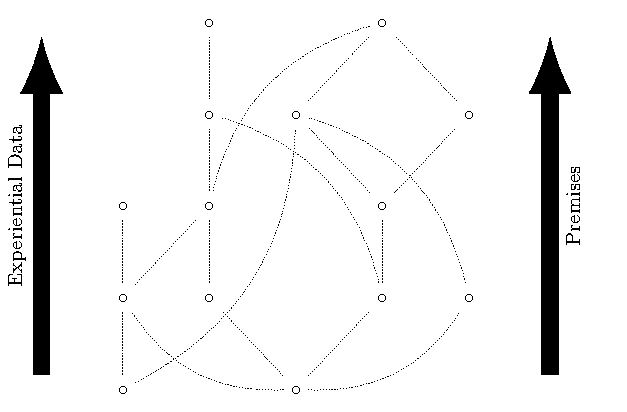
\includegraphics[]{poset/poset2.pdf}
\end{center}
\caption{A network of beliefs}
\label{fig:poset}
\end{figure}

I feel the above observation informs a corresponding perspective on
epistemology.  If an agent's world view largely rested legends about
the Norse gods, I'd be reluctant to say she knows various facts about
nature, such as why lightning strikes.  This is because all of her
explanations would inevitably be based upon myths in one way or
another, which would all occupy lower nodes in her belief network.
This dictates that \emph{sanity} plays a role in how much knowledge an
agent can have - it is permissible to grant that an inconsistent agent
has knowledge provided that the inconsistency follows only shallowly
from her experiential data, and it is something she would readily give
up.  However, if a contradiction is intrinsic to the agent's
psychology, and thus follows from a lower node in her belief poset, my
analysis suggests she doesn't really have knowledge.  So while I
believe that irrational agents can possess knowledge, as I have argued
in \S\ref{irrational}, I do not contend that they \emph{always} posses
knowledge. Moreover, I hold that the sort of irrationality that I am
considering needn't be superficial - both mundane as well as deeply
demented characters can be modeled.

I'll admit that the above essentially presents my own interpretation
of Quine's web of belief, which might be contentious.  On the other
hand, I feel both the quote from Quine and the quote from Whitman in
\S\ref{contradictions} suggest the following principle without too
much controversy:
\begin{quote}
 \textbf{Quine/Whitman Principle}: \emph{Epistemic agents are compound
   entities, which invite compositional analysis.}
\end{quote}
The above presents the final philosophical principle that I intend to
extend.  Apart from this, I would say from the previous discussion, I
would like to extract an additional thing:  Figure \ref{fig:poset}
naturally suggests that we might think of \emph{going up} in a belief
net, in a manner similar to how $\BM$ allows one to \emph{go down} as
I suggested in \S\ref{Descartes}. Along these lines, I would suggest
the introduction of a new operator $\BP$.  The semantics for $\BP$ are
given as follows:
\[ \Omega,(a,A) \VDash \BP \phi \iff \textup{ for all }
(b,B)\in\Omega\textup{ if } b = a \textup{ and } A\subseteq B \textup{
  then } \Omega,(a,A) \VDash \phi \]
Just as $\BM$ corresponds to the agent casting assumptions into doubt,
or disregarding their premises, $\BP$ corresponds to the agent
embracing their experience, suspending disbelief and accepting her
intuitions and senses.

This essentially concludes the sketch of novelties I propose in the
practice of modelling knowledge.

\subsection{Closing Remarks}
\label{close}
The various principles extended in the previous sections are not
independent - some of them are more basic than others.  Their
relationship is summarized in Fig. \ref{fig:principles} - here the
lower a principle is depicted, the more basic I feel it is.  Dotted
lines indicate that I feel the philosophical justification for the
higher principle supervenes on the justification of the lower
principle.
\begin{figure}[ht]
\begin{center}
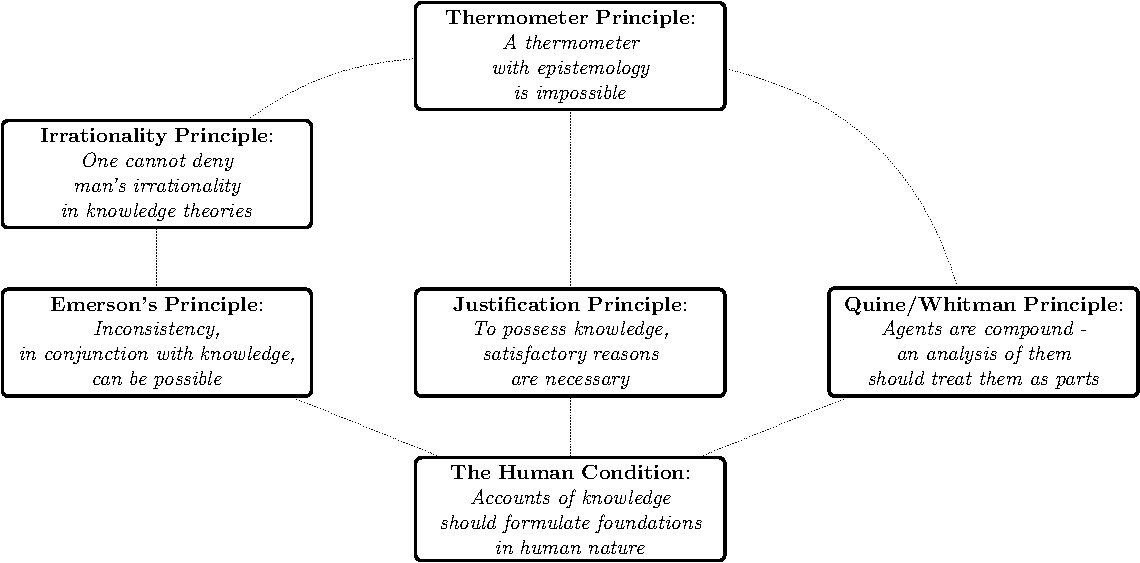
\includegraphics[width=\textwidth]{principles/principles.pdf} 
\end{center}
\caption{A visualization of the relationship of the principles I have suggested}
\label{fig:principles}
\end{figure}
In addition, in further development of the framework sketched in \S\ref{explicit}, I shall want the following criteria, based on my ideas given in relevant sections:
\begin{description}
 \item[\S\ref{explicit}] \begin{bul}
                          \item Agents shall be modelled with proofs for the things they believe.
			  \item To avoid paradoxes, correct
                            foundations must be provided.  Idealy, I
                            would like my semantics to correspond to a
                            provably terminating computation, granting
                            certain non-deterministic operations such
                            as a  \emph{choice operator}
                            $\varepsilon$, as described in
                            \citep{hilbert_neubegrndung_1922}.
                         \end{bul}
  \item[] For a set of beliefs $A$:
\begin{description}
  \item[\S\ref{soundness}] It should be expressible whether everything in $A$ is sound 
  \item[\S\ref{Descartes}] Certain subsets $B\subseteq A$ should be accessible
  \item[\S\ref{quine}] Certain extensions $B \supseteq A$ could also be accessed
\end{description}
\end{description}
In line with evidentialist epistemology, as mentioned in
\S\ref{sketch}, I have decided to call the logic I shall develop
\emph{Evidentialist Logic}, or \textsc{EviL} for brevity.

\section{Introduction to \textsc{EviL}}\label{evil-semantics}
%\subsection{Forward}
With the philosophical intuitions and scaffolding provided from
\S\ref{philosophy}, I shall now turn to giving a precise account of my previously
developed ideas.  This shall be done in three movements:
\begin{description}
 \item[\S\ref{basic-evil}]  In the first section I will provide the
   basic grammar and semantics for \textsc{EviL} with a single agent;
   the presentation in this section will remain primarily
   philosophical and light.
 \item[\S\ref{dead-by-dawn}]  In the second section I develop several
   topics in the pure theory of \textsc{EviL} which I consider a bit
   beyond the bare essentials.
  \item[\S\ref{army-of-darkness}]  In this section, completeness and
    decidability is discussed in relation to \textsc{EviL} and two sublogics.
\end{description}

% from that section provided by the previous section into a provide an outline
% for the basic grammar and semantics of \textsc{EviL}. I also try to develop
% intuitions about how I personally read these semantics, and provide examples of
% various validities.

%\addcontentsline{toc}{subsection}{15 pgs}at t
\subsection{Elementary \textsc{EviL}}\label{basic-evil}
\subsubsection{Grammar \& Semantics}\label{evil-grammar}
In this section we turn to developing the formal semantics for
\tmtextsc{EviL} with a single agent.  We shall imagine the 
object of study in \textsc{EviL} is an agent, which we shall call the
\textsc{EviL} agent.  In \S\ref{multi-agent}, the semantic framework
offered here is extended to incorporate multiple agents. In Appendix
\ref{alternative}, yet another framework is offered employing gamelike
semantics, which avoids the grammar restriction suggested in \S\ref{sketch}.

The grammar restriction imposed on \textsc{EviL} was introduced to
avoid paradoxes. That being the case, we shall discard the previous
definition of $(\VDash)$ that was suggested in \S\ref{sketch}, in
favor of demonstrably well-defined semantics.  
This shall be achieved in two steps.

\begin{definition} Let $\mathcal{L}_0 (\Phi)$ be the language of
  classical propositional logic, defined by the following Backus-Naur form grammar:
\[ \phi \ {::=} \  p \in \Phi \  | \  \phi
   \rightarrow \psi \  | \  \bot \]
\end{definition}
Models for classical propositional logic can be thought of as sets $S
\subseteq \Phi$;
thus the truth predicate
%{\footnote{Here we are assuming
%    $\textup{\textsf{bool}} := \{True, False\}$.  
% This is more commonly written as
% $(\models) \colons \powerset \Phi \rightarrow (\mathcal{L}_0 (\Phi)
% \rightarrow \textup{\textsf{bool}})$ or $(\models) \colons \powerset \Phi \rightarrow
% \textup{\textsf{bool}}^{\mathcal{L}_0 (\Phi)}$.  The notation I
% present assumes that $\to$ associates to the left, following the
% convention for implication in logic. In general, my notation follows
% the typed functional programming languages \tmtextit{Haskell} 
% and \tmtextit{OCaml}.}
%} 
$(\models) \colons \powerset \Phi \times \mathcal{L}_0 (\Phi)
\rightarrow \textup{\textsf{bool}}$ for classical 
propositional logic can be given recursively as follows:
\begin{definition}\label{classical-semantics}
Define $(\models)$ such that
\begin{align*}
  S{\models}p & {\iff}p{\in}S\\
  S{\models}{\phi}{\rightarrow}{\psi} & {\iff}S{\models}{\phi}\text{ implies
  }S{\models}{\psi}\\
  S{\models}{\bot} & {\iff} False
\end{align*}
\end{definition}
Further, observe that the language $\mathcal{L}_0$ is extended by \tmtextsc{EviL}
\begin{definition} Define $\mathcal{L} (\Phi)$ by the following Backus-Naur grammar:
\[ \phi \ {::=} \  p \in \Phi \  | \  \phi
   \rightarrow \psi \  | \  \bot \  |
   \  \Box \phi \  | \  \boxminus \phi
   \  | \  \boxplus \phi \  | \ 
   \circlearrowleft \]
\end{definition}
Unlike traditional modal logic, \textsc{EviL} employs concrete models
rather than Kripke structures. \tmtextsc{EviL} models are sets 
$\Omega \subseteq \powerset \Phi \times \powerset \mathcal{L}_0
(\Phi)$.  Like classical propositional logic, semantics for
\tmtextsc{EviL} are given recursively by a predicate $(\VDash)$ which:
\begin{itemizedot}
  \item Takes as input:
\begin{itemizedot}
  \item An \evil model
  \item A pair $(a, A)$ where
  \begin{itemizedot}
    \item $a\subseteq \Phi$ is a set of proposition letters
    \item $A\subseteq \mathcal{L}_0 (\Phi)$ is a set of propositional formulae.
  \end{itemizedot}
  \item A formula in the language $\mathcal{L} (\Phi)$
  \end{itemizedot}
  \item Gives as output: a truth value in $\textup{\textsf{bool}}$
\end{itemizedot}

More concisely, this may be written as 
\[ (\VDash) \colons \powerset  (\powerset \Phi \times \powerset \mathcal{L}_0 (\Phi)) \times (\powerset \Phi
   \times \powerset \mathcal{L}_0 (\Phi)) \times \mathcal{L} (\Phi) \rightarrow
   \textup{\textsf{bool}}. \]

% The following provides a  of the semantics for 
% \textsc{EviL}:

\begin{definition}\label{evil-semantics-def}
 Define $(\VDash)$ recursively such that:
\begin{align*}
  {\Omega},(a,A){\VDash} p & {\iff}p{\in}a\\
  {\Omega},(a,A){\VDash} {\phi}{\rightarrow}{\psi} &
  {\iff}{\Omega},(a,A){\VDash}{\phi}\text{ implies
  }{\Omega},(a,A){\VDash}{\psi}\\
  {\Omega},(a,A){\VDash}{\bot} & {\iff} False\\
  {\Omega},(a,A){\VDash}\Box {\phi} & {\iff}{\forall}(b,B){\in}{\Omega}.
  ({\forall}{\psi}{\in}A. b{\models}{\psi})\text{ implies
  }{\Omega},(b,B){\VDash}{\phi}\\
  {\Omega},(a,A){\VDash}{\boxminus}{\phi} &
  {\iff}{\forall}(b,B){\in}{\Omega}. a=b\text{ and }B{\subseteq}A\text{
  implies }{\Omega},(b,B){\VDash}{\phi}\\
  {\Omega},(a,A){\VDash}{\boxplus}{\phi} &
  {\iff}{\forall}(b,B){\in}{\Omega}. a=b\text{ and }B{\supseteq}A\text{
  implies }{\Omega},(b,B){\VDash}{\phi}\\
  {\Omega},(a,A){\VDash}{\circlearrowleft} & {\iff}
  {\forall}{\psi}{\in}A.a{\models}{\psi}
\end{align*}
\end{definition}
\begin{remark}
We will write $\Omega \VDash \phi$ to mean $\Omega, (a,A) \VDash \phi$
for all $(a,A) \in \Omega$.  Further, we will write $\VDash \phi$ to
mean $\Omega \VDash \phi$ for all $\Omega$.
\end{remark}
These semantics are well defined, since apart from relying on the semantics
for propositional logic they may be observed to be compositional.
Moreover, the following relationship can be observed:

\begin{lemma}[Truthiness]\label{truthiness}
  Let $\phi \in \mathcal{L}_0 (\Phi)$.  Then:
  \[ a \models \phi \Longleftrightarrow \Omega, (a, A) \VDash \phi \]
  for any $\Omega$ and $A$.
\end{lemma}
\begin{proof}
  This may be seen immediately by induction on $\phi$.
\end{proof}

With this, we have the following result:
\begin{definition}
 $$Th(\Omega) := \{ \phi \in \mathcal{L}(\Phi) \ |\ \Omega \VDash \phi \}$$
\end{definition}

\begin{theorem}[Theorem Theorem]\label{theorem-theorem}
  If $A$ is finite, then $\Omega, (a,A) \VDash \Box \phi$ if and only if $Th(\Omega) \cup A \vdash_{\text{\textsc{EviL}}} \phi$.
\end{theorem}
\begin{proof}
  The proof proceeds the exactly as the proof of Proposition
  \ref{central-prop} from \S\ref{sketch}.
\end{proof}

I shall present $\vdash_{\text{\textsc{EviL}}}$, the logical consequence turnstile for \textsc{EviL}, in \S\ref{evil-axioms}.

I chose the name ``Theorem Theorem'' because it means that for every
belief the \textsc{EviL} agent has, it is a theorem she has derived
from her premises. Theorem \ref{theorem-theorem} establishes one of
the central desiderata outlined in \S\ref{close} is achieved by
\textsc{EviL}.  With this result the foundation is set for the the
central intuition driving \textsc{EviL} - that beliefs are the
consequences of logical deductions.  It is a peculiarity of
\textsc{EviL} that these deductions are carried on in \textsc{EviL}
itself.  This was achieved, primarily, by flirting heavily with
paradox, as was illustrated in \S\ref{sketch}.  
As a consequence, we have tried to design \textsc{EviL}
to eat its own tail. 
It establishes that the \textsc{EviL} agent is
herself also a modeler just like us, using the same logic we are using
to think about her herself, to think about the state space she lives
in.

This sort of self referential circularity is a celebrated theme in
mathematics. It is similar, in a way, to the old alchemical conception
of mathematics, exemplified by the following quote 
due to Sir Thomas Browne:
\begin{quote}
All things began in order, so shall they end, and so shall they begin
again; according to the ordainer of order and mystical Mathematicks of
the City of Heaven.\cite[chapter 5]{browne_garden_1736}\end{quote}
Another, related notion of self reference was championed by Douglas
Hofstadter in his book \emph{G\"odel, Escher, Bach: An Eternal Golden
  Braid}, in what he calls ``Strange Loops'':
\begin{quote}
The flexibility of intelligence comes from the enormous number of
different rules, and levels of rules. The reason that so many rules on
so many different levels must exist is that in life, a creature is
faced with millions of situations of completely different types. In
some situations, there are stereotyped responses which require "just
plain" rules. Some situations are mixtures of stereotyped
situations-thus they require rules for deciding which of the ``just
plain'' rules to apply. Some situations cannot be classified-thus
there must exist rules for inventing new rules \ldots and on and
on. Without doubt, Strange Loops involving rules that change
themselves, directly or indirectly, are at the core of
intelligence. Sometimes the complexity of our minds seems so
overwhelming that one feels that there can be no solution to the
problem of understanding intelligence-that it is wrong to think that rules of any sort govern a creature's behavior, even if one takes ``rule''
in the multilevel sense described above. \cite[pg. 24]{hofstadter_godel_1979}
\end{quote}
In the setting of \textsc{EviL}, the strange loop is as follows: the
rules of the logic affect, indirectly, the truths of the semantics,
which in turn affect the rules of the logic.  It is perhaps dangerous
to engage in this sort of modeling, since it invites paradox.
However, the central goal of epistemic logic is to
provide a logic which models agents with knowledge.  This is because we are
ourselves agents with knowledge; epistemic logic's ultimate purpose is
to say ourselves by studying the subject.  \textsc{EviL} was designed
with to make true the Theorem Theorem, precisely with this final
reason in mind.

It cannot be stressed enough, Theorem \ref{theorem-theorem} is central
to the conceptual backing behind \textsc{EviL}.  
It provides the conceptual backbone of the perspective on 
epistemic logic this essay is intended to investigate.

%%% Local Variables: 
%%% mode: latex
%%% TeX-master: "evil_philosophy"
%%% End: 
\subsubsection{Intuitions}
\label{evil-intuition}
In this section, I shall illustrate how I intuitively read the operators in
\tmtextsc{EviL}, and provide a number of validities.

As per the traditional doxastic reading of $\Box  \phi$, I read this as
asserting ``The \tmtextsc{EviL} agent believes $\phi$''.  Because of Theorem
\ref{theorem-theorem}, the Theorem Theorem, I shall freely conflate this with the assertion
``The \tmtextsc{EviL} agent has an argument for $\phi$,'' which I take to be a
proof.

My intuition for how to read $\DM \phi$ was first mentioned in
\S\ref{Descartes} with respect to Descartes' Meditation II -- it means ``If the
\tmtextsc{EviL} agent were to set aside some of her beliefs, or cast some of
her beliefs into doubt, then $\phi$ would hold.''  Dually, I tend to read
$\boxminus \phi$ as saying something like ``For all the ways that the
\tmtextsc{EviL} agent might use her imagination, $\phi$ holds.''  I recognize
that these interpretations might seem inconsistent -- however, I regard
casting beliefs into doubt and embracing one's imagination as part of the same
coin.  For, naturally, when one doubts more things, then for a fleeting moment their dreams take flight as the inconceivable turns around into the conceivable, if only for a little while.  To give an example, if I set aside for a moment my belief that

{\hspace*{\fill}}the law of gravity is an exceptionless regularity of the
universe, {\hspace*{\fill}}$(g)$

then it seems natural to imagine that

{\hspace*{\fill}}a propulsion device exploiting some exception to gravitation might be constructable.{\hspace*{\fill}}$(p)$

In the symbology of \tmtextsc{EviL} formulae, I would code this intuition as
\[ \boxminus (\Box  \neg g \rightarrow \diamondsuit p) . \]
To give another example, if I pretend that it isn't the case that:

{\hspace*{\fill}}the canals of Amsterdam are filthy{\hspace*{\fill}}$(f)$

I might be able to imagine a scenario where

{\hspace*{\fill}}I am swimming comfortably in the Amstel
river{\hspace*{\fill}}$(r)$

But not really.  I really can't really swim at ease in the Amstel, not just
because it has tons of garbage, but also because

{\hspace*{\fill}}I don't own a bathing suit,{\hspace*{\fill}}$(b)$

Frankly, I am not so bold that I could go skinny dipping in Amstel without
that being awkward.  Hence I would say in the language of \tmtextsc{EviL}
that:
\[ \neg \boxminus (\Box  \neg f \rightarrow \diamondsuit r) \]
This is because I can cast into doubt the assumption of the filthiness of the
canals of Amsterdam, while still retaining my belief that I don't have a
bathingsuit, so swimming in Amstel would still be awkward for me.  In
symbols, I would write express this sentiment as the following expression:
\[ \DM (\diamondsuit \neg f \wedge \Box  b \wedge \neg \diamondsuit r)
\]
Further, my intuition for how to read $\DP \phi$ is ``If the
\tmtextsc{EviL} agent were to remember something, then $\phi$ would hold.'' \
For instance, I can think of an instance where I woke up and searched myself
for my bike keys.  To my horror, they weren't there -- in I immediately
assumed that I might have left my keys in the lock on my bike, and figured
there was a fair likelihood that

{\hspace*{\fill}}my bike has been stolen because I left the keys in
it.{\hspace*{\fill}}$(s)$

But once I recalled that

{\hspace*{\fill}}I had lent my bike to a friend,{\hspace*{\fill}}$(l)$

my fear subsided.  I would have said that prior to remembering, while
I thought it might be possible that my bike was stolen due to my negligence,
if I remembered what I had done then I no longer would have entertained that
possibility.  I would express this observation as:
\[ \diamondsuit s \wedge \boxplus (\Box  l \rightarrow \Box  \neg s) \]
I consider $\boxminus$ and $\boxplus$ to be inverse modalities of each other,
in exactly the same way that \tmtextit{past} and \tmtextit{future} are inverse
modalities in temporal logic. This is perhaps a little unusual; it is arguably
more natural to think of \tmtextit{forgetting} as the inverse modality of
remembering, and there doesn't appear to be an natural inverse operation
corresponding to casting into doubt.  Following the idea of the \tmtextit{web
of belief} due to Quine, as presented in \S\ref{quine}, I would extend a position
asserting that remembering factive data is the same as embracing as much of
one's evidence as possible.

In terms of the semantics outlined, $\boxminus$ corresponds to a subsetset
relation while $\boxplus$ corresponds to a superset relation.  Because of
this, I sometimes read $\boxminus \phi$ closer to the formal semantics, as
saying something like ``for all subsets of the agent's beliefs, $\phi$ holds''
and dually for $\boxplus \phi$.  This is admittedly even less natural than
the reading of remembering as the opposite of casting into doubt.  So be it;
I am comfortable with \tmtextsc{EviL} agents being at best twisted cartoon
versions of actual people, who actually have minds and engage in remembering,
imagining, and other similar activities.  After all, according to the
semantics stipulated in \S\ref{evil-grammar}, \tmtextsc{EviL} agents apparently have sets
for brains, which makes an \tmtextsc{EviL} agent a strange effigy for a person
indeed -- with the possible exception of set theorists, whose brains are
typically constructed entirely of sets or urelements.

Furthermore, it is under the set theoretical reading that $\PP$ makes
the most sense.  I read it as asserting something like ``the basis for
the \textsc{EviL} agent's beliefs is sound'' or ``the \textsc{EviL}
agent's arguments only use true premises.''  It further means that the
actual state of affairs is compatible with what the agent believes -
reality has not been ruled out by something that the agent is taking
as evidence.  Moreover, sound premises intuitively exhibit the
following property - any subset of them is also sound, since soundness
isn't a phenomenon that is subject to synchronicity or other failures
of compositionality.  A set of premises is sound if and only if all of
its subsets are also sound.

%%% Local Variables: 
%%% mode: latex
%%% TeX-master: "evil_philosophy"
%%% End: 

\subsubsection{Validities}
\label{validities}
The previous philosophical readings of \textsc{EviL} immediately
suggest certain validities will hold in the semantics.  For instance, the
assertion ``A set of premises is sound if and only if all of its
subsets are sound.'' would be expressed as
\begin{equation}
\VDash \PP \IFF \BM \PP \label{ppequiv}
\end{equation}
Indeed, this is a validity of \textsc{EviL}.  Schematically, it may be
tempting to think that maybe the same is true for $\BP$.  However, we
have that:
\begin{equation}
\nVDash \PP \to \BP \PP \label{notPPBPPP}
\end{equation}
Nor does this make much sense.  It asserts ``If the agent's basic beliefs
are sound, then all extensions of her basic beliefs are sound too.''
Soundness is a fragile thing -- it is rather easy to think of things
to add to a sound set of basic beliefs which break soundness, such as
``All logicians are centaurs''  and other such demonstrably false nonsense.

Related to \eqref{ppequiv}, there is another related validity  
associated with $\PP$; namely that if the
\textsc{EviL} agent's assumptions are sound, then anything she
concludes from them is true (employing the reading which naturally
arises from Theorem \ref{theorem-theorem}).  This is expressed as
\begin{equation}
\VDash \PP \to \Box \phi \to \phi \label{axiom-11}
\end{equation}
The formula \eqref{ppequiv} expresses that the soundness of one's
premises  is something \emph{persistent} as the \textsc{EviL} agent
carries on casting doubt on assumptions and discarding them.  Another
thing that is persistent this way is the \text{EviL} agent's
imagination:
\begin{equation}
\VDash \Pos \phi \to \BM \Pos \phi \label{axiom-8}
\end{equation}
I read \eqref{axiom-8} as saying something like ``If the \textsc{EviL}
agent can conceive/imagine something, then no matter what things she casts into
doubt, she can still imagine it.''  One can also express something
like the dual of this, namely
\begin{equation}
\VDash \Box \phi \to \BP \Box \phi
\end{equation}
We shall read the above as asserting ``If the agent \emph{can compose
  an argument} then she will still be able to compose that argument if
she remembers more information and experiences she's had in the world.''  
This should not be surprising -- this is yet another expression of the 
Theorem \ref{theorem-theorem}, the Theorem Theorem, and the fact that
the proof theory of \textsc{EviL} is monotonic.
In general, many of the assertions
here exhibit interplay between $\BP$ and $\Box$, and dually $\BM$ and
$\Pos$  -- further investigation of these relationships is taken up in \S\ref{elimination}.

For better or for worse, \textsc{EviL} semantics make
true the following assertion: if something is achievable by repeatedly casting
assumptions into doubt, then it's achievable by casting assumptions
into doubt only once:
\begin{equation}
\VDash \PM^+\phi \to \PM \phi
\end{equation}
Here $^+$ is taken from the syntax for \emph{regular
  expressions} commonly used in computer science and UNIX programming
to mean ``one or
more'' \citep{friedl_mastering_2006}.  Similarly, I have assumed that
discarding no assumptions is, in a way, vacuously casting assumptions
into doubt.  In light of this \textsc{EviL} also makes true the following:
\begin{equation}
\VDash \phi \to \PM \phi
\end{equation}
Furthermore, it is worth mentioning some harder to understand
validities of this system.  The first one is that when the agent
believes something, they believe it regardless of the process of
doubting or embracing their beliefs:
\begin{eqnarray}
\VDash \Box \phi \to \Box \BM \phi \label{dontcare1}\\
\VDash \Box \phi \to \Box \BP \phi \label{dontcare2}
\end{eqnarray}
We can observe that this generalizes to multiple agents, as specified
in \S\ref{multi-agent}.

Another more challenging validity is the fact that if
some proposition $\phi$ holds, then for any restriction of the
\textsc{EviL} agent's beliefs (or dually, any extension), 
if those beliefs are sound, then $\phi$ must be conceivable (i.e.,
$\Pos \phi$ holds).  This is
expressed as the following two validities:
\begin{eqnarray}
\VDash \phi \to \BM (\PP \to \Pos \phi) \label{fraghack1}\\
\VDash \phi \to \BP (\PP \to \Pos \phi) \label{fraghack2}
\end{eqnarray}
Finally, another a peculiarity of \textsc{EviL} is that not all of its
validities are \emph{schematic}.  For instance, there is a kind of
\emph{Cartesian dualism} present in the semantics, where the
\textsc{EviL} agent's deliberation on her evidence does not bear on
brute matters of fact.  For a world pair $(a,A)$, $A$ and $a$ are
basically separate - an \textsc{EviL} agent's mind and the world they
live are composed of different substance.  This gives rise to the following four validities: 
\begin{eqnarray}
& \VDash p \to \BM p \\
& \VDash p \to \BP p \\
& \VDash \neg p \to \BM \neg p \\
& \VDash \neg p \to \BP \neg p
\end{eqnarray}
Hence, \textsc{EviL} is not a \emph{normal} logic.  This should
admittedly be considered a wart on the semantics, since it appears
that it rules out the conventional algebraic duality most modal logics
exhibit (see \citet{blackburn_modal_2001}, chapter 5).  

On the other hand, it is by the same assumption of Cartesian dualism
that underlies the non-normality that \eqref{ppequiv}
as is a natural consequence.  By accepting non-normality, and the
grammar restriction we have imposed on \emph{basic beliefs} to avoid
paradoxes, it follows as a consequence that a belief set is sound if
and only if all of its subsets are sound.  Hence non-normality for
\textsc{EviL} has two aspects -- it compromises the algebraic elegance
of the semantics, while simultaneously giving rise to a philosophically
appealing principle.

In the next section, we turn to a more systematic study of the
validities of \textsc{EviL}.  We shall see that this gives rise to an
\emph{elimination theorem}.
%%% Local Variables: 
%%% mode: latex
%%% TeX-master: "evil_philosophy"
%%% End: 

\subsection{\textsc{EviL} Basics}
\label{dead-by-dawn}
\subsubsection{Elimination}
\label{elimination}
% \documentclass{letter}
% \usepackage{geometry,amsmath,amssymb}
% \geometry{letterpaper}
% 
% %%%%%%%%%% Start TeXmacs macros
% \newcommand{\assign}{:=}
% \newcommand{\colons}{\,:\,}
% \newcommand{\tmop}[1]{\ensuremath{\operatorname{#1}}}
% \newcommand{\tmtextsc}[1]{{\scshape{#1}}}
% \newenvironment{itemizedot}{\begin{itemize} \renewcommand{\labelitemi}{$\bullet$}\renewcommand{\labelitemii}{$\bullet$}\renewcommand{\labelitemiii}{$\bullet$}\renewcommand{\labelitemiv}{$\bullet$}}{\end{itemize}}
% \newenvironment{proof}{\noindent\textbf{Proof\ }}{\hspace*{\fill}$\Box$\medskip}
% \newtheorem{definition}{Definition}
% \newtheorem{lemma}{Lemma}
% \newtheorem{theorem}{Theorem}
% %%%%%%%%%% End TeXmacs macros

%\begin{document}

In this section, I illustrate that the structural validities of \textsc{EviL} can be used to reason that $\BM, \BP, \DM,$ and $\DP$ exhibit certain behavior over two dual fragments of the language $\mathcal{L}(\Phi)$.

The following lemma summerizes the structural validities, in a systematic fashion, that I will be studying in the subsequent discussion:

\begin{lemma}
  \label{validities}The following validities hold for all \tmtextsc{EviL}
  models:
  \[ \begin{array}{lll}
       \VDash \boxminus p \leftrightarrow p & \hspace{5em} & \VDash \boxplus p
       \leftrightarrow p\\
       \VDash \boxminus \neg p \leftrightarrow \neg p &  & \VDash \boxplus
       \neg p \leftrightarrow \neg p\\
       \VDash \boxminus \diamondsuit \phi \leftrightarrow \diamondsuit \phi & 
       & \VDash \boxplus \Box \phi \leftrightarrow \Box \phi\\
       \VDash \DM \Box \phi \leftrightarrow \Box \phi &  &
       \VDash \DP \diamondsuit \phi \leftrightarrow \diamondsuit
       \phi\\
       \VDash \boxminus \boxminus \phi \leftrightarrow \boxminus \phi &  &
       \VDash \boxplus \boxplus \phi \leftrightarrow \boxplus \phi\\
       \VDash \boxminus \DP \phi \leftrightarrow \DP \phi &  & \VDash \boxplus \DM \phi
       \leftrightarrow \DM \phi\\
       \VDash \boxminus \circlearrowleft \leftrightarrow \circlearrowleft &  &
       \VDash \boxplus \neg \circlearrowleft \leftrightarrow \neg
       \circlearrowleft
     \end{array} \]
\end{lemma}

These validities suggest a definite interplay between the modalities of
\tmtextsc{EviL} -- this section is devoted to establishing a certain
expression of this interplay that follows from the interplay expressed above.

First note that the usual substitution rule holds:

\begin{lemma}
  If $\VDash \phi \leftrightarrow \psi$ is a validity, then $\VDash \chi
  \leftrightarrow \chi [\phi / \psi]$ is a validity for any $\chi \in
  \mathcal{L} (\Phi)$.
\end{lemma}

Next, I
offer the following definition of two sublanguages of the main language of
\tmtextsc{EviL}:

\begin{definition}
  Define the following fragments:\footnote{The fragment $\mathcal{L}_A(\Phi)$ was inspired from the continuous fragment of $\mu \tmop{PML}$ (FIXME).}
  
  $\mathcal{L}_A (\Phi)$:
  \[ \phi {::=} \  p \  | \  \neg p
     \  | \  \top \  | \  \bot
     \  | \  \circlearrowleft \  | \ 
     \phi \wedge \psi \  | \  \phi \vee \psi \ 
     | \  \diamondsuit \phi \  | \  \boxminus
     \phi \  | \  \DP \phi \]
  $\mathcal{L}_B (\Phi)$:
  \[ \phi {::=} \  \neg p \  | \  p
     \  | \  \bot \  | \  \top
     \  | \  \neg \circlearrowleft \  |
     \  \phi \vee \psi \  | \  \phi \wedge \psi
     \  | \  \Box \phi \  | \  \DM \phi \  | \  \boxplus \phi \  \]
\end{definition}

\begin{definition}
  Define two dualizing operations $(\cdot)^A : \mathcal{L}_B (\Phi)
  \rightarrow \mathcal{L}_A (\Phi)$ and $(\cdot)^B : \mathcal{L}_A (\Phi)
  \rightarrow \mathcal{L}_B (\Phi)$, using recursion, such that:
  \[ \begin{array}{ll}
       \neg p^A \assign p & p^B \assign \neg p\\
       p^A \assign \neg p & \neg p^B \assign p\\
       \bot^A \assign \top & \top^B \assign \bot\\
       \top^A \assign \bot & \bot^B \assign \top\\
       \neg \circlearrowleft^A \assign \circlearrowleft & \circlearrowleft^B
       \assign \neg \circlearrowleft\\
       (\phi \vee \psi)^A \assign \phi^A \wedge \psi^A & (\phi \wedge \psi)^B
       \assign \phi^B \vee \psi^B\\
       (\phi \wedge \psi)^A \assign \phi^A \vee \psi^A & (\phi \vee \psi)^B
       \assign \phi^B \wedge \psi^B\\
       (\Box \psi)^A \assign \diamondsuit (\psi^A) & (\diamondsuit \psi)^B
       \assign \Box(\psi^B)\\
       (\DM \psi)^A \assign \boxminus (\psi^A) & (\boxminus
       \psi)^B \assign \DM (\psi^B)\\
       (\boxplus \psi)^A \assign \DP (\psi^A) & (\DP \psi)^B \assign \boxplus (\psi^B)
     \end{array} \]
\end{definition}

With the above definition in hand, observe the following natural duality
theorem:

\begin{lemma}
  Observe that for all $\phi \in \mathcal{L}_A (\Phi)$ and $\psi \in
  \mathcal{L}_B (\Phi)$, $(\phi^B)^A = \phi$ and $(\psi^A)^B = \psi$. \
  Moreover, we have the following validities: $\VDash \neg (\phi^B)
  \leftrightarrow \phi$ and $\VDash \neg (\psi^A) \leftrightarrow \psi$.
\end{lemma}

\begin{proof}
  The above follows from routine induction.
\end{proof}

The above duality is convenient, since it means that results proven for one
fragment $\mathcal{L}_A (\Phi)$ can be transfered to $\mathcal{L}_B (\Phi)$ in
a straight-forward manner.

Here is what I see as the consequence of the logical equivalence given in
Lemma \ref{validities}:

\begin{definition}
  If $\phi \in \mathcal{L}_X (\Phi)$ then let $\phi^{\ast}$ be the same
  formula, with all instances of $\boxplus$, $\boxminus$, $\DM$
  and $\DP$ eliminated.
\end{definition}

\begin{theorem}[Vanishing]\label{vanishing}
  For all $\phi \in \mathcal{L}_A (\Phi)$ or $\phi \in \mathcal{L}_B (\Phi)$,
  we have the following validity:
  \[ \VDash \phi \leftrightarrow \phi^{\ast} \]
\end{theorem}

\begin{proof}
  To prove proceeds in three steps.
  
  Step 1: First, use induction on $\phi \in \mathcal{L}_A (\Phi)$, and show
  the following two facts simultaneously:
  \begin{align*}
    {\VDash}{\boxminus}{\phi}{\leftrightarrow}{\phi} &
    {\hspace{3em}}{\VDash}\DP{\phi}{\leftrightarrow}{\phi}
  \end{align*}
  \begin{itemizedot}
    \item Cases $p$, $\neg p$, $\bot$, $\top$, $\circlearrowleft$: \ In all of
    these situations, the result follows from the validities illustrated in
    Lemma \ref{validities}.
    
    \item Cases $\wedge, \vee$: \ For $\boxminus$ the connective $\wedge$ is
    simple, and dually for $\DP$ for the connective $\vee$. \
    This is because in each case one may simply use distribution, such as can
    be done here:
    \begin{align*}
      {\VDash}{\boxminus}({\phi}{\wedge}{\psi}) &
      {\leftrightarrow}{\boxminus}{\phi}{\wedge}{\boxminus}{\psi}\\
      & {\leftrightarrow}{\phi}{\wedge}{\psi}
    \end{align*}
    
    On the other hand, $\vee$ is more interesting for $\boxminus$, and dually
    $\wedge$ for $\DP$.  Using induction, Lemma
    \ref{validities}, and subsitution, and distribution, we have the line of
    reasoning:
    \begin{align*}
      {\VDash}{\boxminus}({\phi}{\vee}{\psi}) &
      {\leftrightarrow}{\boxminus}(\DP{\phi}{\vee}\DP{\psi})\\
      & {\leftrightarrow}{\boxminus}\DP({\phi}{\vee}{\psi})\\
      & {\leftrightarrow}\DP({\phi}{\vee}{\psi})\\
      &
      {\leftrightarrow}\DP{\phi}{\vee}\DP{\psi}\\
      & {\leftrightarrow}{\phi}{\vee}{\psi}
    \end{align*}
    
    \item Case $\diamondsuit$: Once again, this follows immediately from the
    validities of Lemma \ref{validities}, namely $\VDash \boxminus
    \diamondsuit \phi \leftrightarrow \diamondsuit \phi$ and $\VDash \DP \diamondsuit \phi \leftrightarrow \diamondsuit \phi$
    
    \item Cases $\boxminus, \DP$: The final step follows from
    one more application of Lemma \ref{validities}, namely by employing the
    following four validities
    \[ \begin{array}{ll}
         \VDash \boxminus \DP \phi \leftrightarrow \DP \phi & \VDash \DP \DP \phi
         \leftrightarrow \DP \phi\\
         \VDash \boxminus \boxminus \phi \leftrightarrow \boxminus \phi &
         \VDash \DP \boxminus \phi \leftrightarrow \boxminus
         \phi
       \end{array} \]
  \end{itemizedot}
  Step 2: \ With the above, we can prove for any $\phi \in \mathcal{L}_A
  (\Phi)$ that $\VDash \phi \leftrightarrow \phi^{\ast}$.  Once again, the
  proof proceeds by induction, the only steps worth noting involve $\boxminus$
  and $\DP$.  In either case, employing the step can be
  completed using Step 1. For instance, we know that $\VDash \boxminus \phi
  \leftrightarrow \phi$, hence $\VDash \boxminus \phi \leftrightarrow
  \phi^{\ast}$ by induction.
  
  Step 3: \ With the result for $\mathcal{L}_A (\Phi)$ in hand, just observe
  that for $\psi \in \mathcal{L}_B (\Phi)$ we have that $(\psi^A)^{\ast} =
  (\psi^{\ast})^A$. With this, substitution, and duality, we have the
  following chain of reasoning:
  \begin{align*}
    {\VDash}{\psi} & {\leftrightarrow}{\neg}({\psi}^A)\\
    & {\leftrightarrow}{\neg}(({\psi}^A)^{{\ast}})\\
    & {\leftrightarrow}{\neg}(({\psi}^{{\ast}})^A)\\
    & {\leftrightarrow}{\neg}({\neg}((({\psi}^{{\ast}})^A)^B))\\
    & {\leftrightarrow}{\neg}{\neg}{\psi}^{{\ast}}\\
    & {\leftrightarrow}{\psi}^{{\ast}}
  \end{align*}
\end{proof}

\begin{example}
 The following validities of \textsc{EviL} are consequences of Theorem \ref{vanishing}:
\[\VDash \BM\DP\Pos\DP\BM\Pos\Pos\DP\BM\DP\Pos\BM\Pos\BM\DP\BM\Pos\DP\neg p  \IFF \Pos\Pos\Pos\Pos\Pos\Pos\neg p \]
\[ \VDash ((\DM\BP\Nec q\wedge\BP\DM\Nec q)\vee\Nec\BP\DM q)\wedge((\BP\Nec\DM q\vee\Nec\DM\BP q)\wedge\DM\Nec\BP q)  \IFF \Nec q \]
\[ \VDash \BM\DP\Pos t \vee \DM\BP\Box \neg t \]
\end{example}


The way I read Theorem \ref{vanishing} is that $\boxminus$
and $\DP$ is empty modalities on $\mathcal{L}_A (\Phi)$, and dually for $\mathcal{L}_B
(\Phi)$ with $\DM$ and $\boxplus$.  Further, note that
$\mathcal{L}_0 (\Phi) \subseteq \mathcal{L}_A (\Phi) \cap \mathcal{L}_B
(\Phi)$ (up to translation), which means that all four of $\boxplus$,
$\boxminus$ along with their duals $\DP$ and $\DM$
vanish on the propositional language.  Inspecting the semantics, this is to
be expected, since neither $\boxplus$ nor $\boxminus$ interact with propositional truth values.

% \end{document}

%%% Local Variables: 
%%% mode: latex
%%% TeX-master: "evil_philosophy"
%%% End: 

\subsubsection{Multiple Agents}\label{multi-agent}
In this section I turn to extending the semantics for
\tmtextsc{EviL} from a single agent, as presented in \S\ref{evil-grammar}, to
accommodate multiple agents.  This is primarily of interest since further
results in \textsc{EviL}, namely completeness, can naturally be
abstracted beyond the single agent case.  But I will freely admit that
my \textsc{EviL} intuitions are principally grounded in the single
agent case -- I recommend thinking about the multi-agent case as just
a generalization of the single agent case.

The following provides the definition of the language of multi-agent \textsc{EviL}:
\begin{definition} Define $\mathcal{L} (\Phi, \mathcal{A})$ by the following Backus-Naur grammar:
\[ \phi \ {::=} \  p \in \Phi \  | \  \phi
   \rightarrow \psi \  | \  \bot \  |
   \  \Box_X \phi \  | \  \boxminus_X \phi
   \  | \  \boxplus_X \phi \  | \ 
   \circlearrowleft_X \]
Here $X \in \mathcal{A}$, and $\mathcal{A}$ is non-empty.
\end{definition}

As in the single agent case, multi-agent \tmtextsc{EviL} models are 
sets $\Omega
\subseteq \powerset \Phi \times   (\powerset
\mathcal{L}_0 (\Phi))^\mathcal{A}$ -- that is, $\Omega$ is a set of
pairs of sets of proposition letters, and indexed sets of
propositional formulae.
 
The semantic entailment relation for
multi-agent \textsc{EviL} is 
\[ (\VDash) \colons \powerset ( \powerset \Phi \times  
   (\powerset \mathcal{L}_0 (\Phi))^\mathcal{A}) \times \powerset \Phi
   \times ( \powerset \mathcal{L}_0 (\Phi))^\mathcal{A}
   \times \mathcal{L} (\Phi, \mathcal{A}) \rightarrow
   \textup{\textsf{bool}}. \]
The input/output behavior of $(\VDash)$ is just as it was defined before in
\S\ref{evil-grammar}, the only difference in this setting is that instead of
taking a pair as an input, where the second element is a
set, it takes an indexed set.

I shall now provide a formal definition of the semantics for the multi-agent $(\VDash)$:
{\footnote{Where $X \in \mathcal{A}$, I
use $A_X$ to denote $A (X)$ provided that $A \colons \mathcal{A} \rightarrow
\powerset \mathcal{L}_0 (\Phi)$}}
\begin{definition}
\begin{align*}
  {\Omega},(a,A){\VDash} p & {\iff}p{\in}a\\
  {\Omega},(a,A){\VDash} {\phi}{\rightarrow}{\psi} &
  {\iff}{\Omega},(a,A){\VDash}{\phi}\text{ implies
  }{\Omega},(a,A){\VDash}{\psi}\\
  {\Omega},(a,A){\VDash}{\bot} & {\iff} False\\
  {\Omega},(a,A){\VDash}\Box_X {\phi} & {\iff}{\forall}(b,B){\in}{\Omega}.
  ({\forall}{\psi}{\in}A_X. b{\models}{\psi})\text{ implies
  }{\Omega},(b,B){\VDash}{\phi}\\
  {\Omega},(a,A){\VDash}{\boxminus}_X{\phi} &
  {\iff}{\forall}(b,B){\in}{\Omega}. a=b\text{ and }B_X{\subseteq}A_X\text{
  implies }{\Omega},(b,B){\VDash}{\phi}\\
  {\Omega},(a,A){\VDash}{\boxplus}_X{\phi} &
  {\iff}{\forall}(b,B){\in}{\Omega}. a=b\text{ and }B_X{\supseteq}A_X\text{
  implies }{\Omega},(b,B){\VDash}{\phi}\\
  {\Omega},(a,A){\VDash}{\circlearrowleft}_X & {\iff}
  {\forall}{\psi}{\in}A_X.a{\models}{\psi}
\end{align*}
\end{definition}

Just as in \S\ref{evil-grammar}, Lemma \ref{truthiness} and Theorem
\ref{theorem-theorem} can be seen to obtain for the new generalized
semantics.  Furthermore, all of the validities mentioned in \S\ref{validities}
and \S\ref{elimination} hold, along with Theorem \ref{vanishing}, 
where $\Box$, $\Pos$, $\BM$,$\BP$, $\DM$, $\DP$ and $\PP$ 
are all replaced with $\Box_X$, $\Pos_X$, $\BM_X$, $\BP_X$,
$\DM_X$, $\DP_X$ and $\PP_X$ respectively, for any fixed 
$X \in \mathcal{A}$.
Furthermore, compactness still fails, just as presented in 
\S\ref{non-compactness}.

Finally, there is are two novel validities that these semantics give
rise to:

\begin{eqnarray*} & \VDash \Box_X \phi \to \Box_X \BM_Y \phi \\
& \VDash \Box_X \phi \to \Box_X \BP_Y \phi 
 \end{eqnarray*}

This is just to say, that the \textsc{EviL} agent's deliberative
process is opaque to other's beliefs, just as in the single agent
case. This was expressed by
\eqref{dontcare1} and \eqref{dontcare2} in \S\ref{validities}. 
The agent cannot read anyone else's mind, nor anyone
else hers.

% I will admit that little use shall be made of \textsc{EviL} generalized
% this way, since the single agent case is far more natural to think
% about for me.  

Using the multi-agent semantics we have developed here, 
the proof theory for \textsc{EviL} that shall be presented in 
\S\ref{army-of-darkness} can now be given in higher generality.

%%% Local Variables: 
%%% mode: latex
%%% TeX-master: "evil_philosophy"
%%% End: 

\subsubsection{Kripke Structures}\label{kripke}
In this section, I will demonstrate that every \textsc{EviL} model
corresponds to some highly structured Kripke model, with a minor
modification on the standard definition.  However, it will turn out
that this correspondence is one way - the class of Kripke models for
which \textsc{EviL} is strongly complete do not, in general,
possess corresponding \textsc{EviL} models.

However, to elucidate my intuition for understanding \textsc{EviL} models as
Kripke models, I would like to return to the visualization technique for
\textsc{EviL} models I introduced in \S(FIXME).  This involved, roughly,
thinking of the \textsc{EviL} models as \emph{posets} with arrows,
as I first presented in Fig. \ref{fig:example1}.  I have given
additional examples in Figs. \ref{fig:example2} and
\ref{fig:example3}.  
In all of these depictions, the implicit relational structure of \textsc{EviL} models is given
visual expression.  So it seems only natural to me that this graphically perceived structure
could also find formal expression.
\begin{figure}[ht]
\centering
\subfigure[A fairly simple example]{
  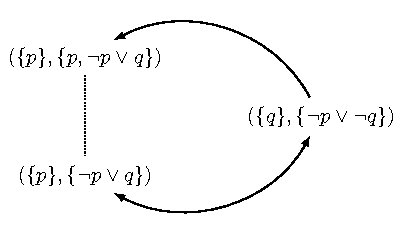
\includegraphics[]{evil_pictures/first_fig.pdf}
%\caption{A fairly simple example}
\label{fig:example2}
}
\subfigure[A more complex example]{
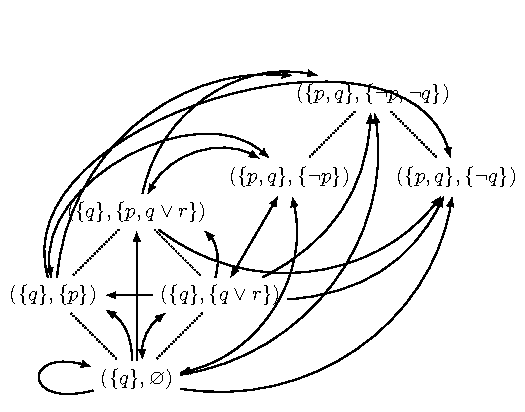
\includegraphics[]{evil_pictures/second_fig.pdf}
\label{fig:example3}
}
\caption{\textsc{EviL} model visualizations}
\end{figure}

Following the modified semantics provided in \S\ref{multi-agent}, the
developments this section will assume multiple agents.
\begin{definition}
  Let $\Phi$ be a set of letters and let $\mathcal{A}$ be a set of agents. \
  A \textbf{Kripke structure} is a state transition system $\mathbb{M}=\langle W^{\mathbb{M}}, R^{\mathbb{M}},
  \sqsubseteq^{\mathbb{M}}, \sqsupseteq^{\mathbb{M}}, V^{\mathbb{M}},
  P^{\mathbb{M}}_{\circlearrowleft} \rangle$ where\footnote{Where
    the context is clear, I shall drop $\mathbb{M}$ from the
    superscripts I am employing.}:
  \begin{itemizedot}
    \item $W^{\mathbb{M}}$ is a set of worlds    
    \item $R^{\mathbb{M}} : \mathcal{A} \rightarrow \powerset (W \times W)$, $\sqsubseteq^{\mathbb{M}} : \mathcal{A} \rightarrow \powerset (W \times W)$, and $\sqsupseteq^{\mathbb{M}} : \mathcal{A} \rightarrow \powerset (W \times W)$ are
    $\mathcal{A}$-indexed sets of relations\footnote{I will abbreviate
      $R(X)$, $\sqsubseteq(X)$ and $\sqsupseteq(X)$ as $R(X)$,
      $\sqsubseteq(X)$ and $\sqsupseteq(X)$ as $R_X$, $\sqsubseteq_X$
      and $\sqsupseteq_X$ respectively.}
    \item $V : \Phi \rightarrow \powerset (W)$ is a predicate letter valuation
    \item $P_{\circlearrowleft} : \mathcal{A} \rightarrow \powerset
      (W)$ are sets of worlds indexed by agents
  \end{itemizedot}
  Let $\mathcal{K}_{\Phi, \mathcal{A}, I}$ denote the class of Kripke structures for letters $\Phi$, agents $\mathcal{A}$, and where $W \subseteq I$.
\end{definition}
Kripke semantics given by $(\Vdash) : \mathcal{K}_{\Phi, \mathcal{A}, I} \to I
\rightarrow \text{\tmtextsf{bool}}$ for these models are defined recursively
as usual, granted the exceptional behavior of $P_{\circlearrowleft}$.
\begin{definition}
  Let $\mathbbm{M}$ be in the class $\mathcal{K}_{\Phi, \mathcal{A}, I}$
  \begin{eqnarray*}
    \mathbbm{M}, w \Vdash p & \Longleftrightarrow & w \in V^{\mathbbm{M}}
    (p)\\
    \mathbbm{M}, w \Vdash \phi \rightarrow \psi & \Longleftrightarrow &
    \mathbbm{M}, w \Vdash \phi \text{ implies } \mathbbm{M}, w \Vdash \psi\\
    \mathbbm{M}, w \Vdash \bot & \Longleftrightarrow & \text{False}\\
    \mathbbm{M}, w \Vdash \Box_X \phi & \Longleftrightarrow & \forall v \in
    W^{\mathbbm{M}} . w R^{\mathbbm{M}}_X v \text{ implies } \mathbbm{M}, v
    \Vdash \phi\\
    \mathbbm{M}, w \Vdash \boxminus_X \phi & \Longleftrightarrow & \forall v
    \in W^{\mathbbm{M}} . w \sqsupseteq^{\mathbbm{M}}_X v \text{ implies }
    \mathbbm{M}, v \Vdash \phi\\
    \mathbbm{M}, w \Vdash \boxplus_X \phi & \Longleftrightarrow & \forall v
    \in W^{\mathbbm{M}} . w \sqsubseteq^{\mathbbm{M}}_X v \text{ implies }
    \mathbbm{M}, v \Vdash \phi\\
    \mathbbm{M}, w \Vdash \circlearrowleft_X & \Longleftrightarrow & w \in
    P_{\circlearrowleft}^{\mathbbm{M}} (X)
  \end{eqnarray*}
\end{definition}
Kripke structures can be observe to have a lot less structure than
\tmtextsc{EviL} models.  However, \tmtextsc{EviL} models can be understood as
Kripke structures in disguise.  To illustrate this, observe the following
lemma:
\begin{definition}[$\mho^\Omega$ Translation]
Let $\Omega$ be an \tmtextsc{EviL} model.  Define
  $\mho^{\Omega} \assign \langle \Omega, R^{\Omega},
  \sqsubseteq^{\Omega}, \sqsupseteq^{\Omega}, V^{\Omega},
  P_{\circlearrowleft}^{\Omega} \rangle$, where
  \[ \begin{array}{llll}
       \bullet & \text{$(a, A) R^{\Omega}_X (b, B) \Longleftrightarrow \forall
       \psi \in A_X .b \models \psi$} & \bullet & (a, A)
       \sqsubseteq^{\Omega}_X (b, B) \Longleftrightarrow a = b \text{ and }
       A_X \subseteq B_X\\
       \bullet & (a, A) \sqsupseteq^{\Omega}_X (b, B) \Longleftrightarrow a =
       b \text{ and } A_X \supseteq B_X & \bullet & (a, A) \in
       P_{\circlearrowleft}^{\Omega} (X) \Longleftrightarrow \forall \psi \in
       A_X .a \models \psi
     \end{array} \]
\end{definition}
\begin{lemma}
  \label{tranlemma1} For all $\Omega$ and all $(a, A) \in \Omega$,  $\Omega, (a, A) \VDash
  \phi$ if and only if $\mho^{\Omega}, (a, A) \Vdash \phi$
\end{lemma}
\begin{proof}
  This follows from a straightforward induction on $\phi$.
\end{proof}
The following summarizes the structural properties of
\tmtextsc{EviL} models, when transformed into Kripke structures:
\begin{proposition}
  For any \textsc{EviL} model $\Omega$,  $\mho^{\Omega}$ has the following
  properties{\footnote{Note that in this we have that $\{w,v\} \subseteq \powerset \Phi
      \times \powerset \mathcal{L}_0$ in the subsequent discussion}}:
  \begin{myRoman}
    \item\label{pI} $\sqsupseteq^{\Omega}_X$ is reflexive
    \item $\sqsupseteq^{\Omega}_X$ is transitive 
    \item \label{pantisym}$\sqsupseteq^{\Omega}_X$ is anti-symmetric
    \item $w \sqsupseteq^{\Omega}_X v$ if and only if $v
    \sqsubseteq^{\Omega}_X w$
    \item If $w \sqsubseteq^{\Omega}_X v$ then $w \in V (p)$ if and only if $v
    \in V (p)$
    \item \label{pV}$R^{\Omega}_X \circ \sqsubseteq^{\Omega}_X \subseteq
    R^{\Omega}_X \subseteq R^{\Omega}_X \circ \sqsupseteq^{\Omega}_X$
    \item $\sqsubseteq^{\Omega}_Y \circ R^{\Omega}_X = R^{\Omega}_X =
    \sqsupseteq^{\Omega}_Y \circ R^{\Omega}_X$
    \item\label{propVII} $w \in P_{\circlearrowleft}^{\Omega} (X)$ if and only if $w
    R^{\Omega}_X w$
  \end{myRoman}
\end{proposition}
\begin{proof}
  Everything except \ref{pV} follows directly from the definitions - so I shall only
  demonstrate $R^{\Omega}_X \subseteq R^{\Omega}_X \circ
  \sqsupseteq^{\Omega}_X$.
  
  Suppose that $(a, A) R^{\Omega}_X (b, B)$, then evidently $\forall \psi \in
  A_X .b \models \psi$. 
  Now assume that $(a, A) \sqsupseteq_X^{\Omega} (c,
  C)$.  Then we know that $A_X \supseteq C_X$.
  But then $\forall \psi \in
  C_X .b \models \psi$, so $(c, C) R^{\Omega}_X (b, B)$, which
  suffices to show the claim.
\end{proof}

\begin{definition}
A Kripke structure is called \tmtextsc{EviL} if it makes true the
  above properties \ref{pI} through \ref{pVII} (with the exception of \ref{pantisym}, which is optional).
\end{definition}

These properties are definitive - as we shall demonstrate, \tmtextsc{EviL} is
sound and weakly complete for \tmtextsc{EviL} models.

The Kripke semantics also serve to \ provide proper intuition behind
\tmtextsc{EviL} models. \ I think of the defined relations given as follows:
\begin{itemizedot}
  \item If $x R^{\Omega}_X y$, then at world $x$ the agent $X$ can imagine $y$
  is true, since $y$ is compatible with what the agent believes 
  \item If $x \sqsubseteq^{\Omega}_X y$, then at world $x$, agent $X$'s
  assumptions (or the experiences they are taking under consideration) are
  contained in her evidence at $y$
\end{itemizedot}
Given this perspective, the proof of \ref{pV} can be understood in the
following way - if the agent assumes fewer things, more things are imaginable,
since it's easier for a world to be incompatible with an agent's evidence.

In fact, in light of Theorem \ref{theorem-theorem}, the above follows
from an underlying, order theoretic relationship present in model theory.  For a given
Kripke structure $\mathbbm{M}$, define two operators $Mod^{\mathbbm{M}}
: \powerset  \mathcal{L} (\Phi, \mathcal{A}) \rightarrow \powerset
(W^{\mathbbm{M}})$ and $Th^{\mathbbm{M}} : \powerset
(W^{\mathbbm{M}}) \rightarrow \powerset \mathcal{L} (\Phi, \mathcal{A})$
\begin{align*}
  Mod^{{\mathbbm{M}}}({\Delta}) &
  =\{x{\in}W{\ }|{\ }{\forall}{\psi}{\in}{\Delta}.
  {\mathbbm{M}},x{\Vdash}{\psi}\}\\
  Th^{{\mathbbm{M}}}({\nabla}) & =\{{\psi}{\in}\mathcal{L}({\Phi},
  \mathcal{A}){\ }|{\ }{\forall}x{\in}{\nabla}.
  {\mathbbm{M}},x{\Vdash}{\psi}\}
\end{align*}
We then have, for any $\Delta \in \powerset  \mathcal{L}
(\Phi, \mathcal{A})$ and $\nabla \in \powerset (W^{\mathbbm{M}})$:
\[ \nabla \subseteq Mod^{\mathbbm{M}} (\Delta) \text{ if and only if }
   \Delta \subseteq Th^{\mathbbm{M}} (\nabla) \]
$\ldots$hence we these two operations form what is refered an
\emph{antitone Galois connection}, between the lattice $\powerset
(W^{\mathbbm{M}})$ and the lattice $\powerset \mathcal{L} (\Phi,
\mathcal{A})$. It follows from the theory of Galois connections
\citep[][chapter 3]{roman_lattices_2008} that
the following two properties:
\begin{itemizedot}
  \item If $\nabla \supseteq \nabla'$ then $Th^{\mathbbm{M}} (\nabla)
  \subseteq Th^{\mathbbm{M}} (\nabla')$
  \item If $\Delta \supseteq \Delta'$ then $Mod^{\mathbbm{M}} (\Delta)
  \subseteq Mod^{\mathbbm{M}} (\Delta')$
\end{itemizedot}
We can see that (\ref{pV}) follows from the second of these two properties. \
To see this, assume that $(a, A) \sqsupseteq_X^{\Omega} (b, B)$, hence $A_X
\supseteq B_X$ and thus $Mod^{\Omega} (A_X) \subseteq
Mod^{\Omega} (B_X)$. \ But it follows from semantics of \tmtextsc{EviL}
we have that $(c, C) \in Mod^{\Omega} (A_X)$ if and only if $(a, A)
R^{\Omega}_X (c, C)$, and likewise for $B_X$. \ Hence if $(a, A) R^{\Omega}_X
(c, C)$ then $(b, B) R^{\Omega}_X (c, C)$.

%%% Local Variables: 
%%% mode: latex
%%% TeX-master: "evil_philosophy"
%%% End: 

\subsection{\textsc{EviL} Completeness}\label{army-of-darkness}
\subsubsection{Failure of Compactness}
\label{non-compactness}
In this section I shall demonstrate that \textsc{EviL} is not compact by giving an example of an infinite set of formulae for which every finite subset is satisfiable while the entirety is not.  %In the subsequent discussion I shall restrict to models with one agent and cease to employ subscripts.

\begin{lemma}%\renewcommand{\qedsymbol}{$\dashv$}
Let $\tau : \Phi \to \mathcal{L}$ be defined as follows:
\begin{center}
\begin{minipage}{3in}
\begin{tabbing}
	$\tau(p) := $ \=$p \wedge \Pos\top \wedge$ \\
	\> $\Nec$ \= $(\neg p \wedge \Pos\top \wedge$\\
	\> \> $\Nec$ \= $(p \wedge \Pos p))$
\end{tabbing}
\end{minipage}
\end{center}
Every finite subset of $\tau[\Phi]$ is satisfiable, but not the entirety, which is infinite. 
\end{lemma}
\begin{proof}
That $\tau[\Phi]$ is infinite is immediate, as $\Phi$ was stipulated to be infinite. 

So let $S\subseteq \tau[\Phi]$ by finite.  We shall find a model that satisfies $S$.  First observe that there is a finite $\Psi\subset \Phi$ such that $S = \tau[\Psi]$. Let $\{q,r,s\} \subseteq \Phi \; \bs \; \Psi$ be three distinct letters - this can be done, since $\Phi \; \bs \; \Psi$ is infinite.  Let $\mathfrak{M}$ be as in Fig. \ref{fig:mod4}, where 
\begin{align*}
a & := \Psi \cup \{s\} \\
b & := \{q \} \\
c & := \Psi \cup \{r\}
\end{align*}
%the valuation function $V$ of $\mathfrak{M}$\footnote{ is such that: $V(p) =\{a,c\}$ for each $p \in \Psi$, $V(q) = \{b\}$, $V(r) = \{c\}$, and $V(s) = \{a\}$.
One may check that $\mathfrak{M},( a,\{q\}) \VDash \tau(p)$ for all $p \in \Psi$.

	\begin{figure}[htbp] %  figure placement: here, top, bottom, or page
   \centering
	\begin{tikzpicture}[->,>=stealth',shorten >=1pt,auto,node distance=4cm,
                    semithick]
  \tikzstyle{every state}=[text=black, shape=rectangle]
  \tikzstyle{empt} = [draw=none,fill=none]
\begin{scope}
\node[empt] (aA1) at (45:2.5) [] {$\pr{a}{\{q\}}$};
\node[empt] (aA2) at (165:2.5) {$\pr{b}{\{r\}}$};
\node[empt] (aA3) at (285:2.5) {$\pr{c}{\{s\}}$};
%\node[empt] (aA4) at (270:2.5) {$\pr{w_4}{\{d\}}$};
\path
(aA1) edge [->,bend right] node {} (aA2)
(aA2) edge [->,bend right] node {} (aA3)
(aA3) edge [->,bend right] node {} (aA1);
%(aA3) edge [->,densely dotted,bend right] node {} (aA4)
%(aA4) edge [->,densely dotted,bend right] node {} (aA1);
\end{scope}
\end{tikzpicture}
\caption{Model $\mathfrak{M}$}
   \label{fig:mod4}
\end{figure}

On the other hand, suppose there was some model $\mathfrak{N}$ such
that $\mathfrak{N}, ( a, A) \VDash \tau(p)$ for all $p \in \Psi$.
This implies that $\mathfrak{N}, ( a, A) \VDash p$ for each $p \in
\Phi$.  Moreover, let $( b, B)$ be such that $\mathfrak{N},( b,
B)\VDash A$ (one exists since by hypothesis $\mathfrak{N}, ( a, A)
\VDash \Pos p$).  By the semantics of $\tau(p)$, it is evident that
$\mathfrak{N}, ( b, B) \VDash \neg p$ and that there's a $( c, C)$
such that $\mathfrak{N},( c,C ) \VDash B$ and $\mathfrak{N},( c,C )
\VDash p \wedge \Pos p$.  But then from this it must be that $a$ and
$c$ both contain exactly the same sentence letters, which means that
$\mathfrak{N},( a,A) \VDash B$ as well.  However it cannot be that
$\mathfrak{N},( a,A ) \VDash \Pos p$ since $\mathfrak{N},( a,A )
\VDash \Nec \neg p$ by $\tau(p)$. Thus it is impossible that
$\mathfrak{N},( a, A) \VDash \tau[\Phi]$. $\lightning$
\end{proof}

This failure of compactness, while a fairly basic result in the model
theory of \textsc{EviL}, is fundamental.  As a consequence, there is
no hope of achieving completeness using infinitary Lindenbaum
constructions that are typically employed in modal logic, such as is
done in \citep[][chapter 4]{blackburn_modal_2001}, for instance.
Any completeness theorem for \textsc{EviL} will necessarily have to be
finite in nature.
\subsubsection{Axiom Systems}\label{evil-axioms}
In this section, we shall present the axiomatics for multi-agent
\textsc{EviL}. The axioms of \textsc{EviL} are presented in 
Table \ref{table:axioms}, which comprises a Hilbert systems for
$\vdash_{\textsc{EviL}}$\footnote{By abuse of notation, we shall omit
  subscripts where they are thought to not be ambiguous}.  In addition
to giving each axiom, we provide a philosophical reading of what each
axiom says.  As remarked in \S\ref{validities}, \textsc{EviL} is not
\emph{normal}, that is it is not closed under variable substitution.

\begin{table}
\newcounter{rownum}
\setcounter{rownum}{0}
\newcounter{rownum2}
\setcounter{rownum2}{0}
\begin{tabularx}{\linewidth}{|cl>{\it}X|}
\hline
(\addtocounter{rownum}{1}\arabic{rownum}) & $\vdash \phi \to \psi \to \phi$ & \multirow{3}{*}{Axioms for basic propositional logic} \\
(\addtocounter{rownum}{1}\arabic{rownum}) & $\vdash (\phi \to \psi \to \chi) \to (\phi \to \psi) \to \phi \to \chi$ &  \\
(\addtocounter{rownum}{1}\arabic{rownum}) & $\vdash (\neg \phi \to \neg \psi) \to \psi \to \phi$ &  \\[6pt]
(\addtocounter{rownum}{1}\arabic{rownum}) & $\vdash \BBI_X \phi \to \phi$ & If $\phi$ holds under any further evidence $X$ considers, then $\phi$ holds simpliciter, since considering no additional evidence is trivially considering further evidence \\[6pt]
(\addtocounter{rownum}{1}\arabic{rownum}) & $\vdash \BBI_X \phi \to \BBI_X \BBI_X \phi$ & If $\phi$ holds under any further evidence $X$ considers, then $\phi$ holds whenever $X$ considers even further evidence beyond that \\[6pt]
(\addtocounter{rownum}{1}\arabic{rownum}) & $\vdash p \to \BB_X p$ & \multirow{2}{8.5cm}{Changing one's mind does not bear on matters of fact}\\
(\addtocounter{rownum}{1}\arabic{rownum}) & $\vdash p \to \BBI_X p$ & \\[6pt]
(\addtocounter{rownum}{1}\arabic{rownum}) & $\vdash \Pos_X \phi \to \BB_X \Pos_X \phi$ & The more evidence $X$ discards, the freer her imagination can run \\[6pt]
(\addtocounter{rownum}{1}\arabic{rownum}) & $\vdash \Nec_X \phi \to \Nec_X \BB_Y \phi$ &  \multirow{2}{8.5cm}{If $X$ believes a proposition, she believes it regardless of what anyone else thinks} \\
(\addtocounter{rownum}{1}\arabic{rownum}) & $\vdash \Nec_X \phi \to \Nec_X \BBI_Y \phi$ & \\[6pt]
(\addtocounter{rownum}{1}\arabic{rownum}) & $\vdash \PP_X \to \Nec_X \phi \to \phi$ & If $X$'s premises are sound, then her logical conclusion are correct \\[6pt]
(\addtocounter{rownum}{1}\arabic{rownum}) & $\vdash \PP_X \to \BB_X \PP_X $ & If $X$'s premises are sound then any subset of will be sound as well \\[6pt]
(\addtocounter{rownum}{1}\arabic{rownum}) & $\vdash \phi \to \BB_X \DDI_X \phi$ &
\multirow{2}{8.5cm}{Embracing evidence is the inverse of discarding evidence} 
\\
(\addtocounter{rownum}{1}\arabic{rownum}) & $\vdash \phi \to \BBI_X \DD_X \phi$ & \\[6pt]
(\addtocounter{rownum}{1}\arabic{rownum}) & $\vdash \Nec_X (\phi \to \psi) \to \Nec_X \phi \to \Nec_X \psi$ &
\multirow{3}{8.5cm}{Variations on axiom $K$}
\\
(\addtocounter{rownum}{1}\arabic{rownum}) & $\vdash \BB_X (\phi \to \psi) \to \BB_X \phi \to \BB_X \psi$ & \\
(\addtocounter{rownum}{1}\arabic{rownum}) & $\vdash \BBI_X (\phi \to \psi) \to \BBI_X \phi \to \BBI_X \psi$ & \\[6pt]
(\addtocounter{rownum2}{1}\Roman{rownum2}) & 
 $\AxiomC{$\vdash \phi \to \psi$}
\AxiomC{$\vdash \phi$}
\BinaryInfC{$\vdash \psi$}
\DisplayProof$ & Modus Ponens\\[10pt]
(\addtocounter{rownum2}{1}\Roman{rownum2}) & 
 $\AxiomC{$\vdash \phi$}
\UnaryInfC{$\vdash \Box_X \phi$}
\DisplayProof$ & \multirow{3}{8.5cm}{Variations on necessitation}\\
(\addtocounter{rownum2}{1}\Roman{rownum2}) & 
 $\AxiomC{$\vdash \phi$}
\UnaryInfC{$\vdash \BB_X \phi$}
\DisplayProof$ &  \\
(\addtocounter{rownum2}{1}\Roman{rownum2}) &
 $\AxiomC{$\vdash \phi$}
\UnaryInfC{$\vdash \BBI_X \phi$}
\DisplayProof$ & \\[10pt]
\hline
\end{tabularx}
\caption{A Hilbert style axiom system for \textsc{EviL}}
\label{table:axioms}
\end{table}


%%% Local Variables: 
%%% mode: latex
%%% TeX-master: "../evil_philosophy"
%%% End: 


Needless to say, these axioms shall be the focus of study for all of
our future investigations in \S\ref{army-of-darkness}.

As a final remark, we should mention that \textsc{EviL} trivially
makes true the \emph{deduction} theorem. This is because we follow
the convention set forth in \cite[Definition 4.4,
pg. 192]{blackburn_modal_2001}, and make the subsequent stipulation:
\begin{mydef}
\[ \Gamma \vdash \phi \iff  \exists \Delta \subseteq_\omega
\Gamma. \vdash \bigwedge \Delta \to \phi \]
\end{mydef}
While trivial, the deduction theorem plays a key role in the proof of
the Theorem Theorem, Theorem \ref{theorem-theorem} from
\S\ref{evil-grammar}.  Specifically, it is this definition that
justifies equation \ref{eq:deduction-theorem2}.

% We immediately have the following theorem:
% \begin{theorem}[Soundness]
% If $\vdash \phi$ then for any model $\mathfrak{M}$ and any 
% $(a,A) \in \mathfrak{M}$ we have that $\mathfrak{M},(a,A) \models \phi$ 
% \end{theorem}

% This logic makes true a variety of relationships between the various
% modalities, which are given in the following lemma:
% \begin{lemma}\label{equivs}
% We have the following provable equivalences:
% \begin{eqnarray*} \vdash \Nec_X \phi \IFF \BB_X \Nec_X \phi & \hspace{1cm} \vdash \Nec_X \phi \IFF \Nec_X \BB_Y \phi \hspace{1cm}  & \vdash \Nec_X \phi \IFF \Nec_X \BBI_Y \phi \\
%  \vdash \BB_X \phi \IFF \BB_X \BB_X \phi & \vdash \BBI_X \phi \IFF
%  \BBI_X \BBI_X \phi & \vdash \PP_X \IFF \BB_X \PP_X\end{eqnarray*}

% &\vdash \PP_X \IFF \DDI_X \PP_X \\
% &\vdash \phi \IFF \psi \textup{ implies } \vdash \chi \IFF \chi[\phi/\psi]
% \end{eqnarray*}
% \ldots where $\chi[\phi/\psi]$ is the same as $\chi$ but every occurrence of $\phi$ as a subformula is replaced by $\psi$.
% $\hfill\dashv$
% \end{lemma}


%%% Local Variables: 
%%% mode: latex
%%% TeX-master: "evil_philosophy"
%%% End: 

In this section we provide a complete axiomatization of
multi-agent \textsc{EviL}.  In addition to axiomatics, we shall also
look at subsystems and supersystems of \textsc{EviL}, and provide
complexity bounds on \textsc{EviL} decision procedures. 

We have organized this section in the following manner:
\begin{description}
 \item[\S\ref{evil-axioms}] We first present a sound axiom
   system for \textsc{EviL}.

 \item[\S\ref{abstraction}] Next, we give a definition of the
   class of \emph{partly \textsc{EviL}} Kripke models.  

   We then reveal that \textsc{EviL} is sound and strongly complete
   for the class of partly \textsc{EviL} models. 
   Completeness rests on the observation that the
   axioms of \textsc{EviL} are all in the \emph{Sahlqvist fragment},
   or have obvious meanings in terms of the traditional canonical
   model construction for Modal Logic.
   This abstract completeness for \textsc{EviL} can be understood as
   an elementary application of van Benthem's 
   \emph{correspondence theory} for modal logic.

\item[\S\ref{completely-evil}]  In this section we recall the definition of an
  \emph{\textsc{EviL} Kripke Model}, as we gave in Definition
  \ref{evil-kripke-structures} from \S\ref{kripke}, and show that
  every \emph{partly \textsc{EviL}} Kripke model may be
  ``completed'' by constructing a bisimilar \emph{\textsc{EviL}} 
   model.

   This has, as a consequence, that \textsc{EviL} is complete for
   \textsc{EviL} Kripke Models.

\item[\S\ref{taking-stock}]  In this section, we discuss why the abstract
  completeness proof developed in the previous sections, while
  important, is not adequate in light of the developments in
  \S\ref{basic-evil} and the intuitions we saw in that section.  We
  shall sketch what further needs to be shown to give the desired
  completeness theorem for \textsc{EviL}.

\item[\S\ref{small-model}]  In this section we show that
  \textsc{EviL} has a small model property for \emph{partly
    \textsc{EviL}} Kripke models. This is accomplished by constructing
     a Kripke model consisting of finite maximally
     consistent sets in the manner of the Fischer-Ladner closure style
     completeness proof of PDL 
     \cite[chapter 4, pgs. 241--248]{blackburn_modal_2001}.

% \item[\S\ref{decidability}] 
%    From our construction in the previous section, we obtain a decidability
%    result for \textsc{EviL}, and provide upper and lower bounds on the
%    complexity of the \textsc{EviL} decision problem.

  \item[\S\ref{islands}] In this section, we introduce the concept of an
    \emph{island}, which are special equivalence classes for
    \textsc{EviL} models.  We shall prove several properties, which take the
    form of irreducibilities. 

\item[\S\ref{translation}]Following the proof of Proposition
  \ref{translation-sketch} in \S\ref{sketch}, we shall show that every
  finite \textsc{EviL} Kripke structure is \emph{(almost)-homomorphic} to another,
  \textsc{EviL} model we shall call $\ipent$, provided that we have an
  infinite number of letters in $\Phi$.  
  We shall show that there is a map $\kl$ of worlds in $\mathbb{M}$ to
  worlds in $\ipent$ that preserves formulae in a language
  $\mathcal{L}(\Psi,\mathcal{A})$ where 
$\Psi \subseteq_\omega \Phi$.

  The construction of $\ipent$ shall make use of the island structures introduced
  in the previous section, and here we will also introduce the concept of
  \emph{names} and \emph{surnames}.

We have, as a consequence of the above, we shall be able to show that
$\textsc{EviL}$ is weakly complete for $\textsc{EviL}$ models.

  % \item[\S\ref{skarmy-of-darkness}]  In this section, we employ our
  %   previous results to remark that \textsc{EviL} is weakly complete for
  %   \textsc{EviL} models.

\item[\S\ref{taking-stockII}]  In this section, we once again pause to
  take stock of the results we have established in previous sections.
  We discuss how our results give rise to complexity observations for
  \textsc{EviL}, and discuss the relationship between the abstract
  completeness we have previously established and our concrete 
  completeness.

  \item[\S\ref{subsystems}] We next introduce two
    subsystems of \textsc{EviL}, corresponding to the $\BP$ and $\BM$
    only fragments. We briefly go over the completeness theorems and
    finite model property for these systems.  In each case, a special
    bisimulation theorem is in order to achieve completeness.

  \item[\S\ref{supersystems}] We provide an extension to
    \textsc{EviL} and its subsystems, introducing the universal
    modality $U$. We sketch completeness and the finite model
    property, and mention how translation may be extended to this
    system.

 \item[\S\ref{lattice}]  In this section we give a lattice of
   \textsc{EviL} systems, and discuss the known complexity bounds of
   various levels of this lattice.
\end{description}

%\subsubsection{Failure of Compactness}
%\label{non-compactness}
%In this section I shall demonstrate that \textsc{EviL} is not compact by giving an example of an infinite set of formulae for which every finite subset is satisfiable while the entirety is not.  %In the subsequent discussion I shall restrict to models with one agent and cease to employ subscripts.

\begin{lemma}%\renewcommand{\qedsymbol}{$\dashv$}
Let $\tau : \Phi \to \mathcal{L}$ be defined as follows:
\begin{center}
\begin{minipage}{3in}
\begin{tabbing}
	$\tau(p) := $ \=$p \wedge \Pos\top \wedge$ \\
	\> $\Nec$ \= $(\neg p \wedge \Pos\top \wedge$\\
	\> \> $\Nec$ \= $(p \wedge \Pos p))$
\end{tabbing}
\end{minipage}
\end{center}
Every finite subset of $\tau[\Phi]$ is satisfiable, but not the entirety, which is infinite. 
\end{lemma}
\begin{proof}
That $\tau[\Phi]$ is infinite is immediate, as $\Phi$ was stipulated to be infinite. 

So let $S\subseteq \tau[\Phi]$ by finite.  We shall find a model that satisfies $S$.  First observe that there is a finite $\Psi\subset \Phi$ such that $S = \tau[\Psi]$. Let $\{q,r,s\} \subseteq \Phi \; \bs \; \Psi$ be three distinct letters - this can be done, since $\Phi \; \bs \; \Psi$ is infinite.  Let $\mathfrak{M}$ be as in Fig. \ref{fig:mod4}, where 
\begin{align*}
a & := \Psi \cup \{s\} \\
b & := \{q \} \\
c & := \Psi \cup \{r\}
\end{align*}
%the valuation function $V$ of $\mathfrak{M}$\footnote{ is such that: $V(p) =\{a,c\}$ for each $p \in \Psi$, $V(q) = \{b\}$, $V(r) = \{c\}$, and $V(s) = \{a\}$.
One may check that $\mathfrak{M},( a,\{q\}) \VDash \tau(p)$ for all $p \in \Psi$.

	\begin{figure}[htbp] %  figure placement: here, top, bottom, or page
   \centering
	\begin{tikzpicture}[->,>=stealth',shorten >=1pt,auto,node distance=4cm,
                    semithick]
  \tikzstyle{every state}=[text=black, shape=rectangle]
  \tikzstyle{empt} = [draw=none,fill=none]
\begin{scope}
\node[empt] (aA1) at (45:2.5) [] {$\pr{a}{\{q\}}$};
\node[empt] (aA2) at (165:2.5) {$\pr{b}{\{r\}}$};
\node[empt] (aA3) at (285:2.5) {$\pr{c}{\{s\}}$};
%\node[empt] (aA4) at (270:2.5) {$\pr{w_4}{\{d\}}$};
\path
(aA1) edge [->,bend right] node {} (aA2)
(aA2) edge [->,bend right] node {} (aA3)
(aA3) edge [->,bend right] node {} (aA1);
%(aA3) edge [->,densely dotted,bend right] node {} (aA4)
%(aA4) edge [->,densely dotted,bend right] node {} (aA1);
\end{scope}
\end{tikzpicture}
\caption{Model $\mathfrak{M}$}
   \label{fig:mod4}
\end{figure}

On the other hand, suppose there was some model $\mathfrak{N}$ such
that $\mathfrak{N}, ( a, A) \VDash \tau(p)$ for all $p \in \Psi$.
This implies that $\mathfrak{N}, ( a, A) \VDash p$ for each $p \in
\Phi$.  Moreover, let $( b, B)$ be such that $\mathfrak{N},( b,
B)\VDash A$ (one exists since by hypothesis $\mathfrak{N}, ( a, A)
\VDash \Pos p$).  By the semantics of $\tau(p)$, it is evident that
$\mathfrak{N}, ( b, B) \VDash \neg p$ and that there's a $( c, C)$
such that $\mathfrak{N},( c,C ) \VDash B$ and $\mathfrak{N},( c,C )
\VDash p \wedge \Pos p$.  But then from this it must be that $a$ and
$c$ both contain exactly the same sentence letters, which means that
$\mathfrak{N},( a,A) \VDash B$ as well.  However it cannot be that
$\mathfrak{N},( a,A ) \VDash \Pos p$ since $\mathfrak{N},( a,A )
\VDash \Nec \neg p$ by $\tau(p)$. Thus it is impossible that
$\mathfrak{N},( a, A) \VDash \tau[\Phi]$. $\lightning$
\end{proof}

This failure of compactness, while a fairly basic result in the model
theory of \textsc{EviL}, is fundamental.  As a consequence, there is
no hope of achieving completeness using infinitary Lindenbaum
constructions that are typically employed in modal logic, such as is
done in \citep[][chapter 4]{blackburn_modal_2001}, for instance.
Any completeness theorem for \textsc{EviL} will necessarily have to be
finite in nature.

\subsubsection{Axioms of \textsc{EviL}}\label{evil-axioms}
In this section, we shall present the axiomatics for multi-agent
\textsc{EviL}. The axioms of \textsc{EviL} are presented in 
Table \ref{table:axioms}, which comprises a Hilbert systems for
$\vdash_{\textsc{EviL}}$\footnote{By abuse of notation, we shall omit
  subscripts where they are thought to not be ambiguous}.  In addition
to giving each axiom, we provide a philosophical reading of what each
axiom says.  As remarked in \S\ref{validities}, \textsc{EviL} is not
\emph{normal}, that is it is not closed under variable substitution.

\begin{table}
\newcounter{rownum}
\setcounter{rownum}{0}
\newcounter{rownum2}
\setcounter{rownum2}{0}
\begin{tabularx}{\linewidth}{|cl>{\it}X|}
\hline
(\addtocounter{rownum}{1}\arabic{rownum}) & $\vdash \phi \to \psi \to \phi$ & \multirow{3}{*}{Axioms for basic propositional logic} \\
(\addtocounter{rownum}{1}\arabic{rownum}) & $\vdash (\phi \to \psi \to \chi) \to (\phi \to \psi) \to \phi \to \chi$ &  \\
(\addtocounter{rownum}{1}\arabic{rownum}) & $\vdash (\neg \phi \to \neg \psi) \to \psi \to \phi$ &  \\[6pt]
(\addtocounter{rownum}{1}\arabic{rownum}) & $\vdash \BBI_X \phi \to \phi$ & If $\phi$ holds under any further evidence $X$ considers, then $\phi$ holds simpliciter, since considering no additional evidence is trivially considering further evidence \\[6pt]
(\addtocounter{rownum}{1}\arabic{rownum}) & $\vdash \BBI_X \phi \to \BBI_X \BBI_X \phi$ & If $\phi$ holds under any further evidence $X$ considers, then $\phi$ holds whenever $X$ considers even further evidence beyond that \\[6pt]
(\addtocounter{rownum}{1}\arabic{rownum}) & $\vdash p \to \BB_X p$ & \multirow{2}{8.5cm}{Changing one's mind does not bear on matters of fact}\\
(\addtocounter{rownum}{1}\arabic{rownum}) & $\vdash p \to \BBI_X p$ & \\[6pt]
(\addtocounter{rownum}{1}\arabic{rownum}) & $\vdash \Pos_X \phi \to \BB_X \Pos_X \phi$ & The more evidence $X$ discards, the freer her imagination can run \\[6pt]
(\addtocounter{rownum}{1}\arabic{rownum}) & $\vdash \Nec_X \phi \to \Nec_X \BB_Y \phi$ &  \multirow{2}{8.5cm}{If $X$ believes a proposition, she believes it regardless of what anyone else thinks} \\
(\addtocounter{rownum}{1}\arabic{rownum}) & $\vdash \Nec_X \phi \to \Nec_X \BBI_Y \phi$ & \\[6pt]
(\addtocounter{rownum}{1}\arabic{rownum}) & $\vdash \PP_X \to \Nec_X \phi \to \phi$ & If $X$'s premises are sound, then her logical conclusion are correct \\[6pt]
(\addtocounter{rownum}{1}\arabic{rownum}) & $\vdash \PP_X \to \BB_X \PP_X $ & If $X$'s premises are sound then any subset of will be sound as well \\[6pt]
(\addtocounter{rownum}{1}\arabic{rownum}) & $\vdash \phi \to \BB_X \DDI_X \phi$ &
\multirow{2}{8.5cm}{Embracing evidence is the inverse of discarding evidence} 
\\
(\addtocounter{rownum}{1}\arabic{rownum}) & $\vdash \phi \to \BBI_X \DD_X \phi$ & \\[6pt]
(\addtocounter{rownum}{1}\arabic{rownum}) & $\vdash \Nec_X (\phi \to \psi) \to \Nec_X \phi \to \Nec_X \psi$ &
\multirow{3}{8.5cm}{Variations on axiom $K$}
\\
(\addtocounter{rownum}{1}\arabic{rownum}) & $\vdash \BB_X (\phi \to \psi) \to \BB_X \phi \to \BB_X \psi$ & \\
(\addtocounter{rownum}{1}\arabic{rownum}) & $\vdash \BBI_X (\phi \to \psi) \to \BBI_X \phi \to \BBI_X \psi$ & \\[6pt]
(\addtocounter{rownum2}{1}\Roman{rownum2}) & 
 $\AxiomC{$\vdash \phi \to \psi$}
\AxiomC{$\vdash \phi$}
\BinaryInfC{$\vdash \psi$}
\DisplayProof$ & Modus Ponens\\[10pt]
(\addtocounter{rownum2}{1}\Roman{rownum2}) & 
 $\AxiomC{$\vdash \phi$}
\UnaryInfC{$\vdash \Box_X \phi$}
\DisplayProof$ & \multirow{3}{8.5cm}{Variations on necessitation}\\
(\addtocounter{rownum2}{1}\Roman{rownum2}) & 
 $\AxiomC{$\vdash \phi$}
\UnaryInfC{$\vdash \BB_X \phi$}
\DisplayProof$ &  \\
(\addtocounter{rownum2}{1}\Roman{rownum2}) &
 $\AxiomC{$\vdash \phi$}
\UnaryInfC{$\vdash \BBI_X \phi$}
\DisplayProof$ & \\[10pt]
\hline
\end{tabularx}
\caption{A Hilbert style axiom system for \textsc{EviL}}
\label{table:axioms}
\end{table}


%%% Local Variables: 
%%% mode: latex
%%% TeX-master: "../evil_philosophy"
%%% End: 


Needless to say, these axioms shall be the focus of study for all of
our future investigations in \S\ref{army-of-darkness}.

As a final remark, we should mention that \textsc{EviL} trivially
makes true the \emph{deduction} theorem. This is because we follow
the convention set forth in \cite[Definition 4.4,
pg. 192]{blackburn_modal_2001}, and make the subsequent stipulation:
\begin{mydef}
\[ \Gamma \vdash \phi \iff  \exists \Delta \subseteq_\omega
\Gamma. \vdash \bigwedge \Delta \to \phi \]
\end{mydef}
While trivial, the deduction theorem plays a key role in the proof of
the Theorem Theorem, Theorem \ref{theorem-theorem} from
\S\ref{evil-grammar}.  Specifically, it is this definition that
justifies equation \ref{eq:deduction-theorem2}.

% We immediately have the following theorem:
% \begin{theorem}[Soundness]
% If $\vdash \phi$ then for any model $\mathfrak{M}$ and any 
% $(a,A) \in \mathfrak{M}$ we have that $\mathfrak{M},(a,A) \models \phi$ 
% \end{theorem}

% This logic makes true a variety of relationships between the various
% modalities, which are given in the following lemma:
% \begin{lemma}\label{equivs}
% We have the following provable equivalences:
% \begin{eqnarray*} \vdash \Nec_X \phi \IFF \BB_X \Nec_X \phi & \hspace{1cm} \vdash \Nec_X \phi \IFF \Nec_X \BB_Y \phi \hspace{1cm}  & \vdash \Nec_X \phi \IFF \Nec_X \BBI_Y \phi \\
%  \vdash \BB_X \phi \IFF \BB_X \BB_X \phi & \vdash \BBI_X \phi \IFF
%  \BBI_X \BBI_X \phi & \vdash \PP_X \IFF \BB_X \PP_X\end{eqnarray*}

% &\vdash \PP_X \IFF \DDI_X \PP_X \\
% &\vdash \phi \IFF \psi \textup{ implies } \vdash \chi \IFF \chi[\phi/\psi]
% \end{eqnarray*}
% \ldots where $\chi[\phi/\psi]$ is the same as $\chi$ but every occurrence of $\phi$ as a subformula is replaced by $\psi$.
% $\hfill\dashv$
% \end{lemma}


%%% Local Variables: 
%%% mode: latex
%%% TeX-master: "evil_philosophy"
%%% End: 


\subsubsection{Partly \textsc{EviL} Kripke Structures \& Strong Completeness}\label{abstraction}\label{partly-evil-strong-soundness-and-completeness}
In this section, we define what it means for a model to be
\emph{partly \textsc{EviL}}.  We should note that partly \textsc{EviL}
models are exactly the same as \textsc{EviL} models as defined in Definition
  \ref{evil-kripke-structures} from \S\ref{kripke}, only property
  \ref{pVII} has been weakened to \ref{ppVII} and \ref{ppIX}.

\begin{definition}[Partly \textsc{EviL}]\label{partly-evil}
A Kripke structure $\mathbb{M}=\langle W, R, \sqsubseteq, \sqsupseteq, V, P \rangle$ is called \textbf{partly
  \textsc{EviL}} whenever it makes true the following properties, for
all agents $\{X,Y\} \subseteq \mathcal{A}$:
  \begin{enumerate}[label=\textup{(\emph{\Roman*})$'$}, topsep=0.0in, parsep=0.075in]
    \item\label{ppI} $\sqsubseteq_X$ is reflexive
    \item \label{pptrans} $\sqsubseteq_X$ is transitive 
    \item \label{ppantisym} $\sqsubseteq$ is a partial order
    \item \label{ppreverse} $w \sqsubseteq_X v$ if and only if $v
    \sqsupseteq_X w$
    \item \label{islandiff} If $w \sqsubseteq_X v$ then ($w \in V (p)$ if and only if $v
    \in V (p)$)
    \item \label{ppV} $(R_X \circ \sqsubseteq_X) \subseteq R_X$
    \item \label{ppVI} $(\sqsubseteq_Y \circ R_X) \subseteq R_X$ and \\
    $(\sqsupseteq_Y \circ R_X) \subseteq R_X$
    \item\label{ppVII} If $w \in P_X$ then $w
    R_X w$
    \item\label{ppIX} If $w \in P_X$ and $w \sqsupseteq_X v$ then $v
    \in P_X$
  \end{enumerate}
\end{definition}

Note that it is elementary that every \textsc{EviL} structure is
partly \textsc{EviL} as well.

These properties are exactly the properties enforced
by the axioms of \textsc{EviL} given in Table \ref{table:axioms} in
\S\ref{evil-axioms}. We can see this by observing the following
theorem:

\begin{definition}\label{pEviL-Vdash}
We shall write
\[ \Gamma \Vdash_{\textup{p\textsc{EviL}}} \phi \]
to mean that for all partly \textsc{EviL} Kripke structures
$\mathbb{M} = \langle W, R, \sqsubseteq, \sqsupseteq, V, P \rangle$,
for all worlds $w \in W$ if $\mathbb{M},w \Vdash \Gamma$ then $\mathbb{M} \Vdash \phi$.
\end{definition}

\begin{theorem}[Partly \textsc{EviL} Strong Soundness and
  Completeness]\label{partly-evil-completeness}

$$\Gamma \vdash_{\textsc{EviL}} \phi\textup{ if and only if }\Gamma
\Vdash_{\textup{p\textsc{EviL}}} \phi$$

\end{theorem}
\begin{proof}
The left to right direction, \emph{soundness}, is trivial (one should
use induction).  So we shall focus on the right to left direction; 
to do this we shall consider the contrapositive.  We shall make heavy
use of \emph{correspondence} theory, namely the \emph{Sahlqvist
  Correspondence Theorem} \cite[Theorem 4.42,
pg. 212]{blackburn_modal_2001}.  We note that the axioms
\eqref{reflAx}, \eqref{transAx}, \eqref{downConceive}, \eqref{islandDown},
\eqref{islandUp}, \eqref{soundness}, \eqref{downsound},
\eqref{reverseAx1} and
\eqref{reverseAx2} are all
\emph{Sahlqvist formulae}.  When we say that a particular fact corresponds to an
axiom, we mean that from the Sahlqvist correspondence theorem and
first order logic one may be employed to show the fact in question.

So assume $\Gamma \nvdash \phi$, 
we must show that $\Gamma \nVdash \phi$.  
To see this, we carry out the canonical model construction as
described in \cite[chapter 4,
pgs. 198--422]{blackburn_modal_2001}\footnote{It is important to note
  that the results obtained in \cite{blackburn_modal_2001} are technically for any \emph{normal} modal logic,
  but they may be generalized to non-normal logics such as the
  \textsc{EviL} logic under consideration.}.  Let $\mathcal{E}$ be the set of maximally
  consistent sets of formulae for \textsc{EviL}. Define the
  \emph{canonical model}
  $$\mathscr{E} := 
\langle \mathcal{E}, R, \sqsubseteq, \sqsupseteq, V, P \rangle$$
where, for all $\{w,v\} \subseteq \mathcal{E}$:
\begin{bul}
  \item $w R_X v$ if and only if $\{ \phi\ |\ \Nec_X \phi \in w\}
    \subseteq v$
  \item $w \sqsubseteq_X v$ if and only if $\{ \phi\ |\ \BP_X \phi \in w\}
    \subseteq v$
  \item $w \sqsupseteq_X v$ if and only if $\{ \phi\ |\ \BM_X \phi \in w\}
    \subseteq v$
  \item $V(p) := \{ w \ |\ p \in w\}$
  \item $P_X := \{ w \ |\ \PP_X \in w \}$
\end{bul}

We know from the \emph{Lindenbaum Lemma} that $\Gamma$ may be extended
to some maximally consistent $\gamma$ such that $\Gamma \subseteq
\gamma$, $\gamma \in \mathcal{E}$ and $\phi \nin
\gamma$ \cite[Lemma 4.17,
pg. 199]{blackburn_modal_2001}.  By the \emph{Truth Lemma} we may establish
$\mathscr{E}, \gamma \nVdash \phi$ and $\mathscr{E}, \gamma \Vdash \Gamma$ \cite[Lemma 4.21,
pgs. 201]{blackburn_modal_2001}.  So it suffices to establish
that $\mathscr{E}$ is partly \textsc{EviL}, by establishing that it
satisfies the properties given in Definition \ref{partly-evil}.

  \begin{description}
    \item[\ref{ppI}] ``$\sqsubseteq_X$ is reflexive''
      corresponds to axiom \eqref{reflAx}.
    \item[\ref{pptrans}] ``$\sqsubseteq_X$ is transitive''
      corresponds to axiom \eqref{transAx}.
    \item[\ref{ppreverse}] ``$\sqsubseteq_X$ is the
      reverse $\sqsupseteq_X$'' corresponds to axioms \eqref{reverseAx1} and
      \eqref{reverseAx2}.
    \item[\ref{islandiff}] Assume $w \sqsubseteq_X v$, we shall show
      that 
$$w \in V (p)\textup{ if and only if }v \in V (p)$$
     Now assume that $w \in V(p)$, then $\mathscr{E}, w \Vdash p$.
      By axiom \eqref{letterAx2} and the Truth Lemma we have that $\BP_X
      p \in w$, whence $p \in v$ by definition.  The other direction
      is similar, however it uses axiom \eqref{letterAx1} instead.
    \item[\ref{ppV}] 
The assertion
\begin{eqnarray*}
& (R_X \circ \sqsubseteq_X) \subseteq
    R_X 
% \\
% & \& \\
% & (R_X \circ \sqsupseteq_X) \subseteq
%     R_X 
\end{eqnarray*}
corresponds to axiom \eqref{downConceive} 
(noting that one should reason given \ref{ppreverse}). 
% This is because axiom \eqref{downConceive} is a Sahlqvist
% formula and together with \ref{ppreverse} it codes for exactly this assertion.

    \item[\ref{ppIX}] ``If $w \in P_X$ and $w \sqsupseteq_X
      v$ then $v \in P_X$'' corresponds to axiom \eqref{downsound}.

     \item[\ref{ppantisym}] We have deferred the proof that
      $\sqsubseteq$ is a partial order, since it depends on the above
      results.  We know that it is reflexive and transitive by
      \ref{ppI} and \ref{pptrans}.  All that is left is to show that
      it is anti-symmetric.  Assume that $w \sqsubseteq v$ and $v
      \sqsubseteq w$.  By the Truth Lemma it suffices to show that
      $\mathscr{E}, w \Vdash \phi$ if and only if $\mathscr{E}, v
      \Vdash \phi$, since then $\phi \in w$ if and only if $\phi \in v$.  We shall show this by induction on $\phi$.
      \begin{description}
        \item[$p \in \Phi$ --]  We have this step from the assumption
          that $w \sqsubseteq v$ and \ref{islandiff}.
        \item[$\bot$ --]  This case is trivially true.
        \item[$\BP_X \phi$ and $\BM_X\phi$ --]  These steps follows from
          \ref{pptrans}, \ref{ppreverse} and the assumption.
        \item[$\Box_X \phi$ --]  This case follows from \ref{ppV} and
          the assumption.
        \item[$\PP_X$ --] This step follows from \ref{ppIX} and the assumption.
        \item[$\phi \to \psi$ --]  The final step follows trivially from the inductive hypothesis.
      \end{description}

    %   Assume that $x \sqsubseteq_X 

% First assume that $w R_X \circ \sqsubseteq_X v$, we must show that $w
% R_X v$.  First observe that we have that there is some
% $u$ such that $w \sqsubseteq_X u$, and $u R_X v$.
%   Now suppose towards a contradiction that $\neg w R_X v$, then there
%   must be some $\Nec_X \phi \in w$ where $\phi \nin v$.  We know
%   that since $u R_X v$ that $\Pos_X \neg \phi \in u$ by the Truth lemma.  However, from axiom
%   \eqref{downConceive} we then have that $\Pos_X \neg \phi \in w$, which
%   violates that $w$ is maximally consistent. $\lightning$

% Now assume that $w R_X v$ and $w \sqsupseteq_X u$.  We must show that
% $u R_X v$.  But we know from $w \sqsupseteq_X u $ and \ref{ppreverse}
% that $u \sqsubseteq_X w$, and with $w R_X v$ we have that $u R_X \circ
% \sqsubseteq_X v$, hence by the above we have $u R_X v$, as desired.


    \item[\ref{ppVI}] Given \ref{ppreverse}, the fact that
    \begin{eqnarray*}
& (\sqsubseteq_Y \circ R_X) \subseteq R_X \\
& \& \\
&  (\sqsupseteq_Y \circ R_X) \subseteq R_X
\end{eqnarray*}
corresponds to axioms \eqref{islandDown} and \eqref{islandUp}.

    \item[\ref{ppVII}] ``If $w \in P (X)$ then $w R_X w$'' corresponds
      to axiom \eqref{soundness}.

  \end{description}

\end{proof}
%%% Local Variables: 
%%% mode: latex
%%% TeX-master: "evil_philosophy"
%%% End: 


\subsubsection{Bisimulation \& \textsc{EviL} Strong Completeness}\label{completely-evil}\label{Abstract-Completeness}
In this section, we show that for every partly \textsc{EviL} Kripke
structure, we may ``complete'' it by constructing a bisimilar
\textsc{EviL} structure; this amounts to enforcing the \textsc{EviL} property \ref{pVII},
namely that a world is reflexive for $R_X$ if and only if it models
$\PP_X$.  This will allow us to establish that \textsc{EviL} is sound
and strongly complete for \textsc{EviL} Kripke models.

We shall first review the definition of \emph{bisimulation}, which we
shall have to modify somewhat given our modified definition of Kripke
structures.  We follow \cite[Definition 2.16, pg.
64]{blackburn_modal_2001} in our presentation:

\begin{mydef}\label{bisimdef}
Let $\mathbb{M} = \langle W, R, \sqsubseteq, \sqsupseteq, V, P
\rangle$ and $\mathbb{M}' = \langle W', R', \sqsubseteq',
\sqsupseteq', V', P' \rangle$.
A non-empty binary relation $Z \subseteq W \times W'$ is a called a
\textbf{bisimulation between $\mathbb{M}$ and $\mathbb{M}'$} (denoted
$Z: \mathbb{M} \leftrightarroweq \mathbb{M}'$) if the following are
satisfied:
\begin{myroman}
  \item If $wZw'$ then $w$ and $w'$ satisfy the same proposition
    letters, along with the special letters $P_X$.
  \item \textbf{Forth} --   
    If $wZ w'$ and $w \leadsto v$, then there exists a $v' \in W'$ such that
    $v Z v'$ and $w' \leadsto' v'$.  
\item \textbf{Back} -- If $wZ w'$ then $w'\leadsto' v'$, then there exists a $v \in W$ such
    that $v Z v'$ and $w \leadsto v$.
\end{myroman}
\ldots where $\leadsto$ is any of $R_X$, $\sqsubseteq_X$, or
$\sqsupseteq_X$, where $X$ is any agent in the class of agents $\mathcal{A}$.
\end{mydef}

We now recall one of the most crucial theorems in all of modal logic:
\begin{theorem}[The Fundamental Theorem of Bisimulations]\label{fundamental-bisim-theorem}
If $Z: \mathbb{M} \leftrightarroweq \mathbb{M}'$ and $w Z w'$, then
for all formulae $\phi$ we have that $$\mathbb{M}, w \Vdash \phi
\textup{ if
and only if }\mathbb{M}', w' \Vdash \phi$$
\end{theorem}
\begin{proof}
This is Theorem 2.20 in \cite[pg. 67]{blackburn_modal_2001}
\end{proof}

We now  introduce a Backus-Naur form grammar for the
$\mathsf{Either}$ type constructor. This will give us precise notation
for manipulating the disjoint union of a Kripke structure $\mathbb{M}$
with itself.

\begin{mydef}\label{eitherdef}
\[ \mathsf{Either}\ a\ b ::= a_l \ |\ b_r \]
\end{mydef}

We now make use of this grammar to express an operation for making bisimilar models:

\begin{mydef}[Bisimulator]
Let $\mathbb{M}$ be a Kripke model, then define a new Kripke model:
$$\invis^\mathbb{M} := \langle W^{\invis}, R^{\invis}, \sqsubseteq^{\invis},
\sqsupseteq^{\invis}, V^{\invis}, P^{\invis} \rangle$$ 
%  as a model
% \[\la W^{\invis^\mathbb{M}},V^{\invis^\mathbb{M}}, P^{\invis^\mathbb{M}}_X,R^{\invis^\mathbb{M}}_{\Nec_X},R^{\invis^\mathbb{M}}_{\BB_X},R^{\invis^\mathbb{M}}_{\BBI_X}\ra\] 
where:
 \begin{eqnarray*}
 W^\invis & := &  \{w_l,w_r\ |\ w\in W^{\mathbb{M}} \} \\
 V^\invis(p) & := &  \{w_l,w_r\ |\ w\in V^{\mathbb{M}}(p)\}\\
 P^\invis_X & := &  \{w_l,w_r \ |\  w\in P^\mathbb{M}_X\}\\
 R^\invis_X & := &  \{(w_l,v_r),(w_r,v_l)\ |\ w R^\mathbb{M}_X v \} \cup \\
 & & \{(w_l,v_l), (w_r,v_r) \ |\ w R^\mathbb{M}_X v
\  \&\  w \in P^\mathbb{M}_X\} \\
 \sqsupseteq_X^\invis & := & \{(w_l,v_l),(w_r,v_r)\ | \ 
 w \sqsupseteq^\mathbb{M}_X v \} \\
 \sqsubseteq_X^\invis & := & \{(w_l,v_l),(w_r,v_r)\ | \ 
 w \sqsubseteq^\mathbb{M}_X v \} 
 \end{eqnarray*}
\end{mydef}

It is instructive to review how $\invis$ operates on
Kripke models it takes as input.  
One idea is that $\invis$ causes every world $w$ in
$\mathbb{M}$ to undergo \emph{mitosis}, and split into two identical
copies named $w_l$ and $w_r$.  These copies obey three rules:
\begin{mynum}
\item The \emph{left copy} of a world $w$, denoted $w_l$, can see
  the \emph{right copy} of a world $v$, denoted $v_r$, provided that
  $w R^\mathbb{M} v$ originally.  This is similarly true for right
  copies, only reflected. 
\item If $\mathbb{M}, w \Vdash \PP_X$, then the copies $w_l$ and $w_r$
  of $w$ can see both $v_l$ and $v_r$ provided that $w R^\mathbb{M} v$
  to begin with.
\item If $w \sqsubseteq_X^\mathbb{M} v$ then
$w_l \sqsubseteq_X^\invis v_l$ and $w_r \sqsubseteq_X^\invis v_r$, but
never $w_l \sqsubseteq_X^\invis v_r$ or $w_r \sqsubseteq_X^\invis
v_l$.
\end{mynum}

The reason $\invis$ duplicates everything in this manner is because
we are preventing $R_X$ reflexivity whenever $w \nin P_X$.
This means that when $w R^\mathbb{M} v$, there are two situations,
which are depicted in Figs. \ref{fig:bisim1} and \ref{fig:bisim2}.
The third rule is depicted in \ref{fig:bisim3}.

For clarity, here is how one should read these three diagrams:
\begin{bul}
 \item If one point $w$ is connected to another point $w'$ by a
   dotted lines with arrows at both ends 
   \tikz \draw[<->,>=latex, dotted ,semithick](0pt,0pt) -- (20pt,6pt);, then
   those points are bisimilar.
 %  this means that $a = b$ and $B \subset A$.
  \item If one point $w$ is connected to another point $v$ by
    a solid line with an arrow and a label $X$ \tikz
    \draw[](0pt,0pt) edge[->,>=latex,semithick] node[xshift=-2.5pt,yshift=-1pt,fill=white,inner sep=.5pt] {\tiny $X$}
    (20pt,6pt) ;, then $w R_X v$, taking care to note which model we are
    reasoning in.
  \item If one point $w$ is connected and \emph{above} to another point $v$ by
    a densely line with no arrow and a label $X$ \tikz
    \draw[](0pt,0pt) edge[densely dotted, semithick] node[fill=white,inner sep=.5pt] {\tiny $X$}
    (20pt,6pt) ;, then $w \sqsupseteq_X v$. 
\end{bul}

\begin{figure}[ht]
\centering
\subfigure[$\mathbb{M},w\Vdash \PP_X$]{
  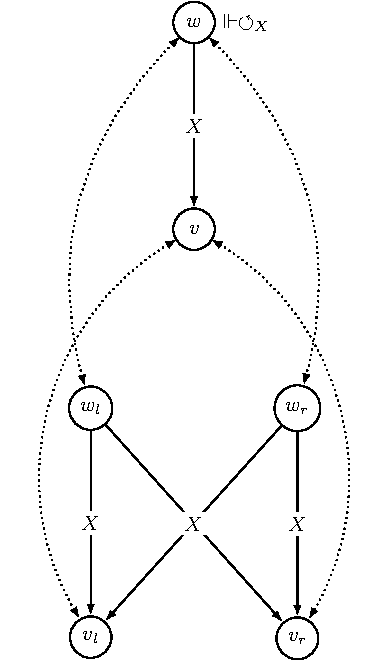
\includegraphics[height=.4\textheight]{evil_pictures/bisim1.pdf}
%\caption{A fairly simple example}
\label{fig:bisim1}
}
\subfigure[$\mathbb{M},w\nVdash \PP_X$]{
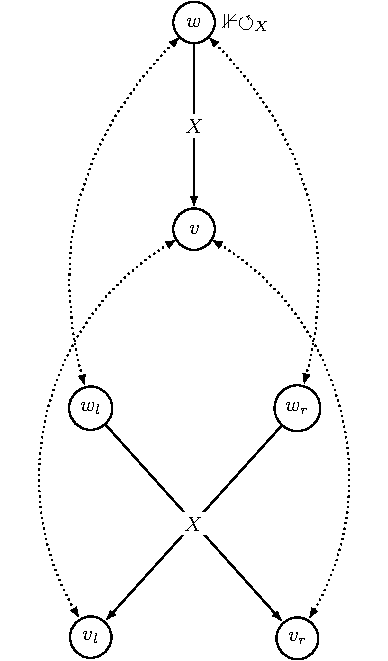
\includegraphics[height=.4\textheight]{evil_pictures/bisim2.pdf}
\label{fig:bisim2}
} 
\subfigure[Always]{
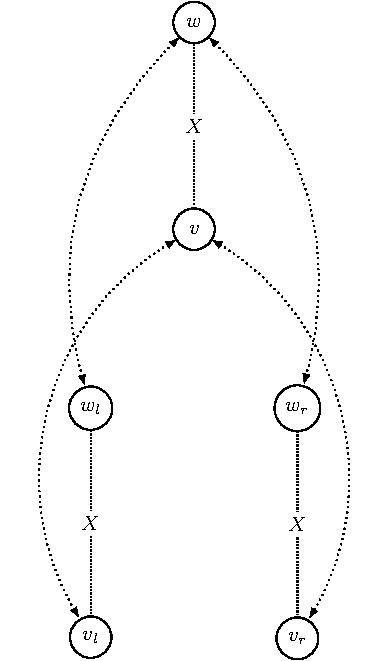
\includegraphics[height=.4\textheight]{evil_pictures/bisim3.pdf}
\label{fig:bisim3}
}

\caption{Visualizations of $\invis$'s operation}
\end{figure}

We summarize the mechanics of $\invis$ in the following proposition:
\begin{proposition}\label{inviskey}
Let $\{w, v\}\subseteq W^\invis$, and let $\{w^\circ, v^\circ\}
\subseteq W^\mathbb{M}$ such that $w^\circ_l = w$ or $w^\circ_r = w$
and similarly for $v^\circ$.
\begin{mynum}
\item If $w$ and $v$ have different handedness, then
\begin{eqnarray*}
&w R^\invis_X v\textup{ if and only if } w^\circ R^\mathbb{M}_X
v^\circ \\
& \& \\
&w \sqsubseteq^\invis_X v\textup{ or }v \sqsubseteq^\invis_X w  \textup{ never holds}
\end{eqnarray*}
\item If $w$ and $v$ have the same handedness, then 
\begin{eqnarray*}
&w R^\invis_X v \textup{ if and only if } w \in
P_X^\mathbb{M}\ \& \ w^\circ R^\mathbb{M}_X v^\circ \\
& \& \\
&w \sqsubseteq^\invis_X v\textup{ if and only if }  w^\circ \sqsubseteq^\mathbb{M}_X v^\circ 
\end{eqnarray*}
\end{mynum}
\end{proposition}

We shall now provide proof that $\invis$ gives rise to a bisimulation:

\begin{lemma}\label{bisimulation}
For any Kripke model $\mathbb{M} = \la W,V,P_X,R_{\Nec_X},R_{\BB_X}, R_{\BBI_X}\ra$, we have the following bisimulation $Z: \mathbb{M} \leftrightarroweq \invis^\mathbb{M}$:
\begin{eqnarray*} w Z w_l & \& & w Z w_r \end{eqnarray*}
\end{lemma}
\begin{proof}
  It follows directly from the definition of $\invis$ that the truth
  of the letters are preserved, along
  with the back and forth conditions for the $\sqsubseteq_X$ and
  $\sqsupseteq_X$ relations.  The proof of the back and forth
  conditions for $R_X$ involves elementary reasoning by cases on whether
  $\mathbb{M}, w \Vdash \PP_X$ or not. This simple argumentation 
  suffices the rest of the proof.
\end{proof}

We now turn to proving that this bisimulation completes a partially
\textsc{EviL} Kripke structure. We shall make use the mechanics of the 
 construction of $\invis$ heavily.

\begin{theorem}[\textsc{EviL} Completion]\label{EviL-Completion}
If $\mathbb{M}$ is partly \textsc{EviL} Kripke structure then
$\invis^\mathbb{M}$ is an \textsc{EviL} Kripke structure. 
\end{theorem}
\begin{proof}
We must verify that $\invis^\mathbb{M}$ makes true all of the
\textsc{EviL} properties.  We may observe that \ref{pI} through
\ref{pislandiff} and \ref{pVI} follow by construction, and 
the fact that since
$\mathbb{M}$ is partly \textsc{EviL} by hypothesis it makes true \ref{ppI} through
\ref{islandiff} and \ref{ppVI}.  All that is left to show is \ref{pV}
and \ref{pVII}.

  \begin{description}
    \item[\ref{pV}] We must show
$$(R^{\invis}_X \circ \sqsubseteq^{\invis}_X) \subseteq
    R^{\invis}_X \subseteq (R^{\invis}_X \circ
    \sqsupseteq^{\invis}_X)$$
Since we already know that $\sqsubseteq^\invis$ is the reverse of
$\sqsupseteq^\invis$, it suffices to show that $(R^{\invis}_X \circ
\sqsubseteq^{\invis}_X) \subseteq   R^{\invis}_X$.  
So assume that $w  \sqsubseteq^{\invis}_X u$ and $u R^{\invis}_X v$. We know that since $w \sqsubseteq^{\invis}_X u$ then by construction
they must have the same handedness.  Without loss of generality assume
that both $w$ and $u$ are \emph{left}, that is there is some
$\{w^\circ,u^\circ\} \subseteq W^\mathbb{M}$ such that $w = w^\circ_l$
and $u = u^\circ_l$. By construction we have that $w^\circ
\sqsubseteq^\mathbb{M} u^\circ$.  It suffices to show that $w R_X^\invis
v$; to do this we shall reason by cases on the handedness of $v$.
  \begin{description}
\item[Opposite --] Assume that $v$ has the opposite handedness, hence $v = v^\circ_r$ for
some $v^\circ\in W^\mathbb{M}$. Then by construction we have that
$u^\circ R_X^\mathbb{M} v^\circ$.  This means that since
$\mathbb{M}$ is partly \textsc{EviL}, it makes true \ref{ppV}, so $w^\circ
R_X^\mathbb{M} v^\circ$.  Hence by construction we have $w R^\invis_X v$.
\item[Same --]  Now assume that $v$ has the same handedness as $w$ and
  $u$, so $v = v^\circ_l$ for some $v^\circ\in W^\mathbb{M}$.  Since
  $u^\circ_l R^\invis_X v^\circ_l$ by assumption, we know from the
  definition of $\invis$ that $u^\circ \in P_X^\mathbb{M}$.  Since
  $\mathbb{M}$ is partly \textsc{EviL} by hypothesis, and $u
  \sqsupseteq_X w$, then from \ref{ppIX} we have that $w \in
  P_X^\mathbb{M}$.  But then we know by \ref{ppV} that $w^\circ
  R^\mathbb{M}_X v^\circ$, hence by construction we have
   $w R^\invis_X v$ as desired.
\end{description}

\item[\ref{pVII}]  We must show that ``$w \in P_X^\invis$ if
  and only if $w \sqsupseteq^\invis_X w$''. We know that the
  left to right direction holds by construction, since by assumption
  $\mathbb{M}$ is partly \textsc{EviL} and hence makes true
  \ref{ppVII}.

  Now assume that  $w \sqsupseteq^\invis_X w$, then since $w$ can see
  something with the same handedness as itself (namely itself), 
by construction we know that $w^\circ \in P_X^\mathbb{M}$ where $w^\circ_l = w$ or
$w^\circ_r=w$.  Whence $w \in P^\invis_X$, which completes the argument.
\end{description}
\end{proof}

With these observations, we may now strengthen Theorem
\ref{partly-evil-completeness} from partly \textsc{EviL} models to
the fully \textsc{EviL} models originally defined in
Definition \ref{evil-kripke-structures} from \S\ref{kripke}:

\begin{definition}\label{EviL-Vdash}
As in Definition \ref{pEviL-Vdash}, we shall write
\[ \Gamma \Vdash_{\textup{p\textsc{EviL}}} \phi \]
to mean that for all partly \textsc{EviL} Kripke structures
$\mathbb{M} = \langle W, R, \sqsubseteq, \sqsupseteq, V, P \rangle$,
for all worlds $w \in W$ if $\mathbb{M},w \Vdash \Gamma$ then $\mathbb{M} \Vdash \phi$.
\end{definition}

\begin{theorem}[\textsc{EviL} Strong Soundness and
  Completeness]\label{evil-completeness}
$$\Gamma \vdash_{\textsc{EviL}} \phi\textup{ if and only if }\Gamma
\Vdash_{\textup{\textsc{EviL}}} \phi$$
\end{theorem}
\begin{proof}
Note that every \textsc{EviL} Kripke model is partly
\textsc{EviL}, so soundness follows immediately from Theorem
\ref{partly-evil-completeness}.

Now assume that $\Gamma \nvdash_{\textsc{EviL}} \phi$, we must show
that there is some witnessing $\textsc{EviL}$ model with a world that
makes this false.   We know from Theorem
\ref{partly-evil-completeness} that there is 
some partly \textsc{EviL} model $\mathscr{E}$ and some
$w$ in $\mathscr{E}$ such that $\mathscr{E},w \nVdash \phi$ and $\mathscr{E},w \Vdash \Gamma$.  We
know from Lemma \ref{bisimulation} that $\mathscr{E} \leftrightarroweq
\invis^\mathscr{E}$, hence by Theorem \ref{fundamental-bisim-theorem},
\emph{The Fundamental Theorem of Bisimulations}, we know that
$\invis^\mathscr{E},w_l \nVdash \phi$ and 
$\invis^\mathscr{E},w_l \Vdash \Gamma$.  
From Theorem \ref{EviL-Completion} 
we may observe that  $\invis^\mathscr{E}$ is
indeed \textsc{EviL}, which means that we have found a suitable
witness for completeness as desired.
\end{proof}

This completes the strong, abstract completeness proof of
\textsc{EviL} in Kripke semantics.  
We shall now turn to taking stock of what we have
shown so far, and discuss why we must go further to give a true proof of
\emph{completeness} of \textsc{EviL}.

%%% Local Variables: 
%%% mode: latex
%%% TeX-master: "evil_philosophy"
%%% End: 


\subsubsection{Taking Stock I}\label{taking-stock}
In the previous sections, we showed that the logic of \textsc{EviL} we
presented in \ref{evil-axioms} was complete for \textsc{EviL} Kripke
models.  In this section we pause for a moment to discuss why we must
go further, and reason what further needs to be shown in order to
establish completeness.

First, recall the semantics we developed in
Definition \ref{evil-semantics-def} in \S\ref{evil-grammar}.
These semantics were carefully crafted to make true the mystical
Theorem \ref{theorem-theorem}, the \emph{Theorem Theorem}.  This
equated $\Box \phi$ with a proof of $\phi$, in the following manner:

\[ \mathfrak{M},(a,A) \VDash \Box_X \phi \iff Th(\mathfrak{M}) \cup A_X \vdash_{\textsc{EviL}} \phi \]

In the above, we assume that $A_X$ is finite. This above property of \textsc{EviL} was enforced to accommodate the \emph{Justification
  Principle} from \S\ref{explicit}, which says that when an agent
believes something, she must have a reason.

This critical insight, driven by our philosophical perspective on
the nature of knowledge, is lost in the abstracta of Kripke
semantics.  The Kripke semantics perspective on
\textsc{EviL} is basically meaningless on its own; 
for why would anyone ever care about \textsc{EviL} Kripke structures,
without the light of the fact that they somehow 
abstract \textsc{EviL} semantics?  
We know that not every \textsc{EviL} Kripke structure 
can be represented by a \textsc{EviL} structure by Proposition
\ref{not-an-evil-model}.  How do we know that \textsc{EviL} Kripke
structures are faithfully abstracting our concrete semantics at all?

The connection of \textsc{EviL} Kripke structures to \textsc{EviL} has
not yet been entirely revealed, but it is as follows: 
\begin{quote}
\emph{\textsc{EviL} models are finitary, concrete objects, and
  \textsc{EviL} Kripke structures are their potentially infinite, abstract idealizations.}
\end{quote}
Succinctly, this relationship is expressed as follows:
\begin{equation} 
\Gamma \Vdash_{\textsc{EviL}} \phi \iff \Gamma \VDash \phi \label{relationship}
\end{equation}
\ldots for all $\phi$ and finite $\Gamma$.

The relationship is important, since Kripke Semantics are the natural
semantics for modal logics, and hence enable one to rapidly reason
about them.  Equation \eqref{relationship} allows us to see  
that, when thinking about \textsc{EviL}, one 
may freely employ strong completeness and neglect
concerns about failure of compactness, with the understanding that
when we restrict ourselves to  finitary circumstances the abstract
semantics and the concrete semantics coincide.

Sections \S\ref{small-model} through \S\ref{translation} shall be
devoted to establishing this relationship between the abstract and
concrete semantics for \textsc{EviL}.
Since we know that the logic of \textsc{EviL} models is not compact
from Theorem \ref{noncompact}, we shall establish a
\emph{small model property} for partly \textsc{EviL} and \textsc{EviL}
Kripke structures in \S\ref{small-model}.  
By modifying the translation system for finite Kripke structures to
\textsc{EviL} modifying we originally gave in the proof of
Proposition \ref{translation-sketch} from \S\ref{sketch}, we shall
show how to translate finite \textsc{EviL} Kripke structures into
\textsc{EviL} models in \S\ref{translation}.  We shall find need to
make use of the concept of \emph{islands}, which we shall introduce in \S\ref{islands}.

After the above developments, we shall once again take stock of our
observations in \S\ref{taking-stockII}.  We shall prove the equation
\eqref{relationship}, and make use of our previous results to
establish complexity bounds on the decision procedure for \textsc{EviL}.

%%% Local Variables: 
%%% mode: latex
%%% TeX-master: "evil_philosophy"
%%% End: 


\subsubsection{Small Model Construction}\label{small-model}
In this section we provide definitions and lemmas related to the
subformula construction $\Cross^\phi$.  We follow
\cite[chapter 5, pgs. 78--84]{boolos_logic_1995} in our approach, 
as well as the
``Fischer-Ladner Construction'' used in the completeness theorem of PDL
\cite[chapter 4, pgs. 241--248]{blackburn_modal_2001}.

We first recall the definition of \emph{pseudo-negation} from the
Fischer-Ladner construction for the completeness of PDL \cite[chapter
4, pg. 243]{blackburn_modal_2001}.  We shall also introduce
\emph{pseudo-boxes}.  All of these are defined as follows:
\begin{mydef}
\begin{eqnarray*}
\sim \phi := \begin{cases} \psi &\textup{ if $\phi = \neg\psi$} \\ \neg \phi & \textup{ o/w} \end{cases} &
\hspace{1cm} \pBB_X \phi := \begin{cases} \phi &\textup{ if $\phi = \BB_X \psi$} \\ \BB_X \phi & \textup{ o/w} \end{cases} \hspace{1cm} &
\pBBI_X \phi := \begin{cases} \phi &\textup{ if $\phi = \BBI_X \psi$} \\ \BBI_X \phi & \textup{ o/w} \end{cases}
\end{eqnarray*}
\end{mydef}
Like pseudo-negation, the idea of pseudo-boxes
is that they raise the semantic behavior of operators to the syntactic
level.  This is summarized in the following lemma:
\begin{lemma}\label{equivs2} 
\begin{eqnarray*} 
\vdash \sim \phi \IFF \neg \phi &
\hspace{1cm} \vdash \pBB_X \phi \IFF \BB_X \phi \hspace{1cm} &
\vdash \pBBI_X \phi \IFF \BBI_X \phi
\end{eqnarray*}
\begin{align*}
\pBB_X \phi = \pBB_X\pBB_X \phi & & \pBBI_X\phi = \pBBI_X \pBBI_X \phi \hfill
\end{align*}
\end{lemma}
\begin{proof}
We remind the reader that $\vdash$ here abbreviates $\vdash_\textsc{EviL}$.
\begin{description}
  \item[$\vdash \sim \phi \IFF \neg \phi$ --] Assume that $\phi$ is
    unnegated, then $\sim \phi = \neg \phi$ and hence we know that
    $\vdash \neg \phi \IFF \neg \phi$, which suffices.  If $\phi =
    \neg \psi$, then we know that $\sim \phi = \psi$, and since in
    classical logic we have that $\vdash \psi \IFF \neg \neg \psi$ we
    have the result.
  \item[$\vdash \pBB_X \phi \IFF \BB_X \phi$ --] If $\phi$ is not
    boxed with $\BB_x$, the result is trivial.  So assume that $\phi =
    \BB_X \psi$, then $\pBB_X \phi = \BB_X \psi$. 
   
   Note that for 
    \textsc{EviL} Kripke structures, for which $\BB_X$ corresponds to
    $\sqsupseteq_X$, then from \textsc{EviL}ness we know that
    $\sqsupseteq_X$ is transitive and reflexive, hence
    $\Vdash_{\textsc{EviL}} \BB_X \psi \IFF \BB_X \BB_X \psi$.  By
    completeness, we know that $\vdash \BB_X \psi \IFF \BB_X \BB_X
    \psi$.  But this suffices exactly what we wanted to prove.

  \item[$\vdash \pBP_X \phi \IFF \BP_X \phi$ --] This result follows
    using exactly the same reasoning as above, only it uses the fact
    that the \emph{dual} of $\sqsupseteq_X$, which is $\sqsubseteq_X$, is
    reflexive and transitive too.

  \item[$\pBM_X \phi = \pBM_X \pBM_X \phi$ --] First assume that $\phi$
     is a $\BM_X$ boxed formula.  Then 
   $\pBM_X \phi = \pBM_X \pBM_X \phi = \phi$.  Next assume that $\phi$
   is not a $\BM_X$ boxed formula, then $\pBM_X \phi = \BM_X \phi$,
   and hence 
\begin{align*}
\pBM_X \pBM_X \phi & = \pBM_X \BM_X \phi \\
& = \BM_X \phi \\
& = \pBM_X \phi
\end{align*}
  \item[$\pBP_X \phi = \pBP_X \pBP_X \phi$ --] The proof of this
    assertion is exactly the same as the proof for $\pBM_X$.
\end{description}
\end{proof}

We shall use these operations above in the subformula construction we
will carry out.  Next, we introduce an operation which will 
allow us to restrict our subformulae to
precisely the finitary number of agents that shall be relevant.

\begin{mydef} Let $\delta(\phi) \subseteq \mathcal{A}$
% , ``the \textbf{dudes} mentioned by $\phi$'', 
be the set of agents that  occur in $\phi$\end{mydef}

We now employ primitive recursion to define the finite set of formulae
that we shall use in our construction, which we have labeled
$\Sigma$.  This operation behaves as follows:
\begin{bul}
\item $\Sigma$ takes as input:
\begin{bul}
  \item A set of agents $\Delta$
   \item A formula $\phi$ where $\phi \in \mathcal{L}(\mathcal{A},\Phi)$ 
\end{bul}
\item $\Sigma$ outputs a set $S$ of $\mathcal{L}(\mathcal{A},\Phi)$
  formulae (that is, $S \subseteq \mathcal{L}(\mathcal{A},\Phi)$)
\end{bul}
We may summarize this concisely as the following type signature:
\[ \Sigma : (\powerset \mathcal{A}) \times
\mathcal{L}(\mathcal{A},\Phi) \to \powerset
\mathcal{L}(\mathcal{A},\Phi) \]

\begin{mydef}\label{EviLSigma}Define $\Sigma( \Delta,\phi)$ using primitive 
recursion as follows:
\begin{align*}
\Sigma(\Delta,p) := &   \{ p, \neg p, \bot, \neg\bot \} \cup \\
& \{ \BB_X p, \neg\BB_X p, \BBI_X p, \neg\BBI_X p  \ |\ X \in \Delta
\} \\
\Sigma(\Delta,\bot) :=  & \{ \bot, \neg\bot \} \\
% \Sigma(\Delta,\PP_X) :=  & \{ \PP_X, \neg\PP_X, \BB_X \PP_X, \neg
% \BB_X \PP_X, \bot, \neg\bot \} \\
\Sigma(\Delta,\PP_X) :=  & \{ \PP_X, \neg\PP_X, \BB_X \PP_X, \neg
\BB_X \PP_X, \bot, \neg\bot \} \\
\Sigma(\Delta,\phi\to\psi) := & \{ \phi\to\psi,\neg(\phi\to\psi) \}
\cup   \Sigma(\Delta,\phi) \cup \Sigma(\Delta,\psi)\\
\Sigma(\Delta,\Nec_X \phi) := & \{ \Nec_X \phi, \neg \Nec_X \phi,
\BBI_X \Nec_X \phi, \neg\BBI_X\Nec_X \phi \} \cup \\
& \{\Nec_X \pBB_Y \phi, \neg\Nec_X \pBB_Y \phi, \\
&\ \; \Nec_X \pBBI_Y \phi, \neg\Nec_X \pBBI_Y \phi, \\
&\ \; \pBB_Y \phi, \neg \pBB_Y \phi, \\
&\ \; \pBBI_Y \phi, \neg\pBBI_Y \phi\ |\ Y \in \Delta \} \cup \\
& \Sigma(\Delta,\phi) \\
\Sigma(\Delta,\BB_X \phi) := & \{ \BB_X \phi, \neg\BB_X \phi\} \cup \Sigma(\Delta,\phi) \\
\Sigma(\Delta,\BBI_X \phi) := & \{ \BBI_X \phi, \neg\BBI_X \phi\} \cup \Sigma(\Delta,\phi)
\end{align*}
\end{mydef}

To understand how the above operates, we assume that the reader has
some background in recursive programming.  Recall how ``subformulae''
are defined for the Fischer-Ladner construction for the completeness
proof of PDL. We can see that authors describe the set of subformulae
$\neg FL(\Sigma)$ as follows:
\begin{quote}  We defined $\neg FL(\Sigma)$, the \emph{closure of
    $\Sigma$}, as the smallest set containing which is Fischer-Ladner
  closed and closed under single negations \cite[pg. 243]{blackburn_modal_2001}.
\end{quote}
Here Fischer-Ladner closed means the construction satisfies certain
subformula properties, such as ``if $\langle \pi_1 ; \pi_2 \rangle
\phi \in \neg FL(\Sigma)$ then $\langle \pi_1 \rangle \langle \pi_2
\rangle \phi \in \neg FL(\Sigma)$.'' We ask the reader who knows a
little about computers, how would one go about programming 
the Fischer-Ladner closure?  
The easiest way to program the Fischer-Ladner closure, in
languages like \textsf{Haskell} or \textsf{OCaml}, would
be to use pattern recognition and (primitive) recursion.  
This is just as we have done, informally, for the \textsc{EviL} subformulae construction.

We argue that writing a concise, programmatic recursive
characterization as we have done for $\Sigma$ is the easiest way to
express the set with the features we desire. 
For one thing, the closure properties we shall
want depend at the top-level on a constant set of agents,
which are calculated at the beginning of the construction.  
Moreover, as we shall see, we shall need some formulae boxed
in certain ways to ensure certain partly \textsc{EviL} properties and
certain formulae boxed in other ways to ensure other partly \textsc{EviL}
properties.  Worse yet -- since we have multiple kinds of pseudo
operators, we cannot enforce closure for all of them.  Managing
the priorities of when a formula should be closed for which operations
roughly amounts to giving the algorithmic characterization we have
carried out above.

In our subsequent proofs, we shall capitalize on combinatoric
properties that our subformulae operation obeys.  Some of these
features are summarized in the following proposition.  
% The proof of these
% assertions is offered as an exercise to our readers. 
%, who we hope are
%rather fond of inductive proofs and sudoku-like activities:

\begin{proposition}\label{inclusions}
$\Sigma(\delta(\phi),\phi)$ is finite.  Moreover, we have the following:
\begin{bul}
        \item $\phi \in \Sigma(\delta(\phi),\phi)$
	\item If $\psi \in \Sigma(\delta(\phi),\phi)$ and $\chi$ is a subformula of $\psi$, then $\chi \in \Sigma(\delta(\phi),\phi)$
	\item If $\psi \in \Sigma(\delta(\phi),\phi)$ then $\sim \psi \in \Sigma(\delta(\phi),\phi)$
	\item If $\BB_X \phi \in \Sigma(\delta(\phi),\phi)$ then $\pBB_X \phi \in \Sigma(\delta(\phi),\phi)$
	\item If $\BBI_X \phi \in \Sigma(\delta(\phi),\phi)$ then $\pBBI_X \phi \in \Sigma(\delta(\phi),\phi)$
\end{bul}
\end{proposition}

We follow \cite[pg. 243]{blackburn_modal_2001} in our definition of
the set of (relativized) maximally consistent sets:

\begin{mydef}[Atoms] Let $At(\Psi)$ denote the maximally consistent subsets of $\Psi$
\end{mydef}
We next have the Finitary Lindenbaum Lemma:
\begin{lemma}[Finitary Lindenbaum Lemma]If $\Gamma \nvdash \phi$ and $\Gamma\subseteq \Sigma(\delta(\phi),\phi)$, then there is a $\gamma \in At(\Sigma(\delta(\phi),\phi))$ such that $\Gamma \subseteq \gamma$ and $\gamma \nvdash \phi$
\end{lemma}
\begin{proof}
The proof of this assertion follows the same proof of the 
finitary Lindenbaum Lemma offered in \cite[Lemma 4.83,
pg. 244]{blackburn_modal_2001} and \cite[chapter 5, pg. 79]{boolos_logic_1995}.
\end{proof}

We now turn to defining the \textsc{EviL} subformula model we shall
use in the subsequent finitary completeness theorem:

\begin{mydef}
Define 
$$\Cross^\phi := \langle W, R, \sqsubseteq, \sqsupseteq, V, P \rangle$$
Where:
\begin{align*}
W := & At(\Sigma(\delta(\phi),\phi)) \\
V(p) := & \{ w \in W \ |\ p \in w \} \\
P_X := & \{ w \in W \ |\ \PP_X \in w \} \cup \{ w\in W \ | \ X \nin \delta(A)\}\\
R_X := & \begin{cases} \{(w,v) \in W \times W \ |\ \{ \psi\ |\ \Box_X \psi \in w\}
\subseteq v \} & \textup{when $X \in \delta(\phi)$}\\
\varnothing & \textup{o/w}
\end{cases}
 \\
\sqsupseteq_X  := & \begin{cases} \{(w,v) \in W \times W \ |\
  \{\psi,\pBB_X \psi \ |\ \pBB_X \psi \in w\} \subseteq v\ \& &
  \multirow{2}{*}{\textup{when $X \in \delta(\phi)$}} \\
 \hspace{3cm}\ \;\;  \{\psi,\pBBI_X \psi \ |\ \pBBI_X \psi \in v\}
 \subseteq w \} \} \\
\{ (w,w) \ |\ w \in W\} & \textup{o/w}
\end{cases} 
\\
\sqsubseteq_X  := & \begin{cases} \{(v,w) \in W \times W \ |\
  \{\psi,\pBB_X \psi \ |\ \pBB_X \psi \in w\} \subseteq v\ \& &
  \multirow{2}{*}{\textup{when $X \in \delta(\phi)$}} \\
 \hspace{3cm}\ \;\;  \{\psi,\pBBI_X \psi \ |\ \pBBI_X \psi \in v\}
 \subseteq w \} \} \\
\{ (w,w) \ |\ w \in W\} & \textup{o/w}
\end{cases} 
\end{align*}
\end{mydef}

In the above construction, we note that the definition of $V(p)$,
$P_X$ and $R_X$ are defined as usual.  Only $\sqsupseteq_X$ and
$\sqsubseteq_X$ have are unusual. Here we are consciously imitating the
completeness techniques given in \cite[chapter 5,
pgs. 78--84]{boolos_logic_1995}, and using 
them for \textsc{EviL}.

We shall now show that $\Cross^\phi$ satisfies the \emph{Truth lemma}.
Once again, the method of the proof of the following theorem is adapted
from \cite[chapter 5, pgs. 78--84]{boolos_logic_1995}.

\begin{lemma}[Truth Lemma]\label{truth}
For any subformula $\psi \in \Sigma(\delta(\phi),\phi)$ and any $w \in
W^{\Cross}$, we have that 
\[\Cross^\phi, w \Vdash \psi \iff \psi \in w\]
\end{lemma}
\begin{proof} The proof proceeds by induction on $\psi$.
\begin{description}
\item[$p \in \Phi$, $\PP_X$, $\bot$ --] These steps are elementary.
\item[$\phi \to \psi$ --] Since we know that $\Sigma(\delta(\phi),\phi)$
   is closed under subformulae, from the inductive hypothesis we have
   that $\Cross^\phi, w \Vdash \phi \iff \phi \in w$ and $\Cross^\phi,
   w \Vdash \phi \iff \phi \in w$.  The rest of the step involves
   reasoning by cases, using the fact that $\Sigma(\delta(\phi),\phi)$ is
   closed under pseudo-negation, $w$ is maximal and pseudo-negation 
   logically equivalent to negation.
\item[$\Box_X\phi$ --]  
  The right to left direction follows by the fact
  that $\Sigma(\delta(\phi),\phi)$ is closed under subformulae, and
  the inductive hypothesis.  Hence we shall concern ourselves with the
  left to right direction.

So assume that $\Box_X \psi \nin w$ we shall show that there is a $v$
such that $w R_x v$ and $\Cross^\phi, v \nVdash \psi$.  Consider the
set 
\[ \Xi := \{ \sim \psi \} \cup \{\chi \ |\ \Box_X \chi \in w\}\]
Note that $\Xi \subseteq \Sigma(\delta(\phi),\phi)$.  If $\Xi$ is consistent, then $\Xi \nvdash \phi$ and we know from the
Lindenbaum Lemma that $\Xi$ may be extended to the $v$ we desire.  

So suppose towards a contradiction that $\Xi$ is not consistent.
Then $\vdash \neg \bigwedge \Xi$, which means by classical logic that: 
$$\vdash \left(\bigwedge_{\Box_X \chi \in w} \chi\right) \to \psi$$
But then we know by modal logic that:
$$\vdash \left(\bigwedge_{\Box_X \chi \in w} \Box_X \chi\right) \to \Box_X \psi$$
This means that since $w \vdash \bigwedge_{\Box_X \chi \in w} \Box_X
\chi$, then we have that $\Box_X \psi \in w$ by maximality after all. This is
ridiculous! $\lightning$

\item[$\BM_X\phi$ --]  This case is similar to the case for $\Box_X \phi$,
  but harder to understand.  

We shall demonstrate the left to right direction, since right to left
is elementary.  
Assume that $\BB_X \psi \nin w$, then we shall find a $v$ such that $w
\sqsupseteq_x v$ and $\Cross^\phi, v \nVdash \phi$.  Since $w$ is
maximal and $\vdash \pBM_X\psi \IFF \BM_X \psi$, we have that $w
\nvdash \pBB_X \psi$.  

Now abbreviate:
\begin{align*}
A := &  \{\chi,\pBB_X \chi \ |\ \pBB_X \chi \in w \}\\
B := & \{ \sim \pBBI_X \chi \ | \ \pBBI_X \chi \in \Sigma(\delta(\phi),\phi)\ \&\ \sim\chi \in w \}
\end{align*}
As before, if $\{\sim \psi\} \cup A \cup B$ consistent then it extends
to the desired $v$.

So suppose towards a contradiction that $\{\sim \psi\} \cup A \cup B
\vdash \bot$.  Then $A \cup B \vdash \psi$, and furthermore by the
equivalences in Lemma \ref{equivs2} and rule \eqref{BMnec} and the
axioms we have that\footnote{Here $\pBB_X S$ is shorthand for $\{
  \pBB_X \chi \ |\ \chi \in S\}$.} $$\pBB_X A \cup \pBB_X B \vdash
\pBB_X \psi.$$ So let 
\begin{align*}
A' := & \{ \pBB_X \chi\ |\ \pBB_X \chi \in w \}\\
B' := & \{ \sim \chi \ | \  \sim\chi \in w \}
\end{align*}
Since $\pBB_X \pBB_X \chi = \pBB_X \chi$ by Lemma \ref{equivs2}, we have $A' = \pBB_X A$.  Moreover, by Lemma \ref{equivs2}, axiom \eqref{reverseAx1}, and classical logic we can see that
\[ \vdash \sim \chi \to \pBB_X \sim \pBBI_X \chi \]
Thus for every $\beta \in \pBB_X B$ we have that $B' \vdash \beta$.  Hence by $n$ applications of the Cut rule we can arrive at 
\[ A' \cup B' \vdash \pBB_X \chi \]
However, evidently $A' \cup B' \subseteq w$, hence $w \vdash \pBB_X
\psi$, which is a contradiction! $\lightning$

To complete the argument, we must show that $w \sqsupseteq_X
v$.  Since $A \subseteq v$ we just need to check that $\{\psi,\pBBI_X \psi \ |\ \pBBI_X \psi \in v\} \subseteq w$.  Suppose
that $\pBBI_X \psi \in v$ but $\psi \nin w$.  Since $w$ is maximally
consistent we have then that $\sim \psi \in w$, hence $ \sim \pBP_X
\in B$ by definition and thus $\sim \pBBI_X
\psi \in v$, since $B \subseteq v$.  This contradicts that $v$ is consistent. $\lightning$

Now suppose that $\pBBI_X \psi \in v$ but $\pBBI_X \psi \nin w$, hence
$\sim \pBBI_X \psi \in w$ and thus $\sim \pBBI_X \pBBI_X \psi \in v$.
However we know from Lemma \ref{equivs2} that $\pBBI_X \pBBI_X \psi =
\pBBI_X \psi$, which once again implies that $v$ is
inconsistent. $\lightning$
\item[$\BP_X\phi$ --]  This is exactly as in the case of $\BM_X\phi$,
  only the appropriate dual assertions of all of the statements used 
are employed.
\end{description}
\end{proof}

We shall now turn to establishing that our finite model is indeed a
partly \textsc{EviL} Kripke structure, following the manner that we
used to show the same result for the
canonical \textsc{EviL} model $\mathscr{E}$.

\begin{lemma}[$\Cross^\phi$ is Partly \textsc{EviL}]\label{cross-is-partly}
$\Cross^\phi$ is a finite partly \textsc{EviL} Kripke structure.
\end{lemma}
\begin{proof}
The fact that $\Cross^\phi$ is finite follows from the fact that
$W^\Cross \subseteq \Sigma(\delta(\phi),\phi)$ and
$\Sigma(\delta(\phi),\phi)$ is itself finite, as we established in Lemma \ref{equivs2}.

The remainder of the proof is devoted to establishing the partly
\textsc{EviL} properties for $\Cross^\phi$.
  \begin{description}
    \item[\ref{ppI}]We must show ``$\sqsubseteq_X$ is reflexive.''
We first note that if $X \nin \delta(\phi)$, then this is true trivially by the
construction of $\Cross^\phi$. 

 So assume that $X \in \delta(\phi)$. We need to show two facts:
\begin{eqnarray*} 
&   \{\psi,\pBB_X \psi \ |\ \pBB_X \psi \in w\} \subseteq w \\
 &  \& \\
&\{\psi,\pBBI_X \psi \ |\ \pBBI_X \psi \in w\}
\subseteq w
\end{eqnarray*}

However, these facts follow from Lemma \ref{equivs2}, the maximality
of $w$ and the fact that we know \textsc{EviL} logic proves:
\begin{eqnarray*}
& \vdash \BB_X \psi \to \psi\\
&\textup{ and } \\
& \vdash \BBI_X \psi \to \psi
\end{eqnarray*}

We know that \textsc{EviL} proves these facts from our
previous completeness theorem, Theorem \ref{evil-completeness}, and 
the fact that $\sqsubseteq_X$ is reflexive for \textsc{EviL} models.

\item[\ref{pptrans}] A quick glance at the definition of
      $\Cross^\phi$ reveals that ``$\sqsubseteq_X$ is transitive''
is immediate by construction.

    \item[\ref{ppreverse}]
Once again, the assertion
``$\sqsubseteq_X$ is the reverse $\sqsupseteq_X$'' 
follows immediately by construction.

    \item[\ref{islandiff}] Assume $w \sqsubseteq_X v$, we shall show
      that 
$$w \in V (p)\textup{ if and only if }v \in V (p)$$

If $X \nin \delta(\phi)$ then we know that $w = v$, so the above is true.

     So assume that $X \in \delta(\phi)$.  
    Now assume that $w \in V(p)$, then $\mathscr{E}, w \Vdash p$.
     This means that $p \in w$, whence $p \in
     \Sigma(\delta(\phi),\phi)$.  
    By Definition \ref{EviLSigma} we have that 
    $\BP_X p = \pBP_X p \in \Sigma(\delta(\phi),\phi)$. 
     By axiom \eqref{letterAx2} and 
     the Truth Lemma (Lemma \ref{truth}),  we have that $\pBP_X
      p \in w$, whence $p \in v$ by construction of $\Cross^\phi$.  The other direction
      is similar, however it uses axiom \eqref{letterAx1} instead.

    \item[\ref{ppV}] 
To prove the assertion
$$ (R_X \circ \sqsubseteq_X) \subseteq
    R_X $$
We first note that if $X \nin\delta(\phi)$, then $R_X \circ
\sqsubseteq_X = R_X = \varnothing$ by construction.  
Hence we may safely assume $X \in \delta(\phi)$.  

Next assume that $w \sqsubseteq_X u$ and $u R_X v$, we need to show that
$w R_X v$.  In order to do this, by construction we need to show that
if $\Box_X \phi \in w$ then $\phi \in v$. However, we know that
$\vdash \Box_X \phi \to \pBP_X \Box_X \phi$ by the logic of
\textsc{EviL}, and by the definition of \ref{EviLSigma} we know
that if $\Box_X \phi \in \Sigma(\delta(\phi),\phi)$ then $\pBP_X\Box_X
\phi \in \Sigma(\delta(\phi),\phi)$ too, so $\pBP_X \Box_X \phi \in w$
by maximality.  However, we then have that $\Box_X \phi \in u$ by
construction, and thus $\phi \in v$ as desired. 
     % \item[\ref{ppantisym}] Just as in the proof of
     %   \ref{partly-evil-completeness} from
     %   \S\ref{partly-evil-strong-soundness-and-completeness}, 
     %  we have intentionally deferred the proof that
     %  $\sqsubseteq$ is a partial order, since it depends on the above
     %  results.  As before, that it is reflexive and transitive by
     %  \ref{ppI} and \ref{pptrans}.  
     %   Moreover, the exact same inductive proof, along with the 
     %  Truth Lemma, may be used to establish anti-symmetry.
    \item[\ref{ppVI}] We must show:
    \begin{eqnarray*}
&(\sqsubseteq_Y \circ R_X) \subseteq R_X \\
& \& \\
& (\sqsupseteq_Y \circ R_X) \subseteq R_X
\end{eqnarray*}

We shall only show that $\sqsubseteq_Y \circ R_X \subseteq R_X$, since
$\sqsupseteq_Y$ is analogous.

First, observe that we may assume that $Y \in \delta(\phi)$, 
since if not then $\sqsubseteq_Y = id$, the identity relation, so 
$\sqsubseteq_Y \circ R_X = R_X$ which suffices.  
Now assume that $\Nec_X \phi \in w$, $w R_X v$ and $v \sqsubseteq_Y
u$; we must show that $\phi \in u$.  
Since $Y \in \delta(\phi)$ then by the construction of $\Sigma$, 
along with the \textsc{EviL} fact that 
$\vdash \Nec_X \phi \to \Nec_X \pBP_X\phi $, we know that 
$Nec_X \pBP_Y \phi \in w$, whence $pBP_Y \phi \in v$.  Since $v
\sqsubseteq_Y u$, we have that $\phi \in u$ as desired.

    \item[\ref{ppVII}] To show ``If $w \in P (X)$ then $w R_X w$,''
    assume $\PP_X \in w$ and $\Nec_X \phi \in w$.  Then we know by
    \textsc{EviL} and maximality that $\phi \in w$, which suffices to
    show that $w R_X w$. 
    \item[\ref{ppIX}] We must show ``If $w \in P_X$ and $w \sqsupseteq_X
      v$ then $v \in P_X$.''  If $w \in P_x$ then by construction we
      know that $\PP_X \in w$.  Note that this can only happen if $X
      \in \delta(\phi)$.  As in the case of \ref{islandiff} we
      know by the definition of $\Sigma$, \textsc{EviL} logic 
      and maximality we have that $ \BM_X \PP_X \in w$.  
      Whence we have $\PP_X \in v$ as desired. 
\end{description}
\end{proof}

We may combine the results above with what we have shown previously in
\S\ref{completely-evil} to give the following series of results:

\begin{theorem}[Weak \textsc{EviL} Soundness and Completeness]\label{abst-finite-completeness}\ 
\begin{center}
\textsc{EviL} is weakly sound and complete for finite \textsc{EviL}
Kripke structures.
\end{center}
\end{theorem}
\begin{proof}
Since soundness is straightforward, we only prove completeness.

Assume that $\nvdash \phi$, in other words we have $\varnothing \vdash
\phi$.  This means by the Lindenbaum Lemma that $\varnothing$ may be
extended to some $w \in At(\delta(\phi),\phi)$ such that 
$\Cross^\phi,w\nVdash \phi$.  We know that $\Cross^\phi$ is partly
\textsc{EviL} from Theorem \ref{cross-is-partly}, so from Theorem
\ref{EviL-Completion} we have that $\invis^\Cross$ is an \textsc{EviL}
model, and since it is bisimilar to $\Cross$ we know that
$\invis^\Cross, w_l \nVdash \phi$.
Now note that for $\invis$ obeys the following rule:  If $|W|$ is
finite then $|W^\invis| = 2 \times |W|$ (since all that $\invis$ is
doing is making duplicates of all of the worlds).  Hence we know that
$\invis^\Cross$ is indeed finite, which means it is a suitable witness.
\end{proof}

\begin{theorem}[\textsc{EviL} Small Model Property]\label{small-model-property}\ 
If $\phi$ is satisfiable by some \textsc{EviL} Kripke structure, then $\phi$ is
satisfied by some finite \textsc{EviL} Kripke structure $\mathbb{M}$ where
$|\mathbb{M}| \in O(EXP2(|\phi|))$
\end{theorem}
\begin{proof}
Assume that $\phi$ is satisfiable in some \textsc{EviL} Kripke
structure, then we know by soundness that $\nvdash \phi$, hence
$\invis^\phi , w \nVdash \phi$ for some $w$ extending $\varnothing$.
So it suffices to show that $|\invis^\phi| \in O(EXP2(|\phi|))$.

Note that $\invis^\phi \subseteq
\powerset(\Sigma(\delta(\phi),\phi))$.  We shall show that
$|\Sigma(\delta(\phi),\phi)| \in O(EXP(|\phi|))$, then we would know
that $|\powerset(\Sigma(\delta(\phi),\phi))| \in O(EXP2(|\phi|))$,
which would suffice to show the result.

First observe that $|\delta(\phi)| \in O(EXP(|\phi|))$.  This is
because in a worst case scenario, $\phi$ is constantly branching into
$\psi \to \chi$ formulae, and adding two new agents every time it
branches.  However, it cannot have more than $3^{|\phi|}$ agents even
in this worst case scenario, so we know that $|\delta(\phi)| \in
O(EXP(|\phi|))$.

To finish the argument, we again perform a worst-case analysis. Every
non-branching step 
(ie. every time $\Sigma$ processes a
 formula not of the form $\psi \to \chi$) 
of $\Sigma(\delta(\phi), \zeta)$ introduces at worst $O(|\delta(\phi)|) \in O(EXP(|\phi|))$
many formulae.  In a worst case
scenario $\Sigma(\delta(\phi),\phi)$ must branch $O(EXP({|\phi|}))$
times and each time perform a $O(EXP(|\phi|))$ operation.  Even in
this worst case scenario, the complexity is still $O(EXP(|\phi|))$,
which is as we claimed.
\end{proof}

\begin{theorem}[\textsc{EviL} Decidability]\label{evil-decidability}\ 
\textsc{EviL} is decidable and 
the time complexity of the decision problem for \textsc{EviL} is
bounded above by $O(EXP3(|\phi|))$
\end{theorem}
\begin{proof}
 We know
that $\Cross^\phi \in \powerset (\powerset
(\Sigma(\delta(\phi),\phi)))$,
we know that
 $\phi$ is not a tautology of \textsc{EviL} if and only if there is a
 suitable \textsc{EviL} witnessing Kripke structure in $\powerset
 (\powerset (\Sigma(\delta(\phi),\phi)))$, defined in the manner of $\Cross$.
So a decision procedure to check if $\phi$ is an \textsc{EviL}
tautology 
is to check every member of
$\powerset (\powerset (\Sigma(\delta(\phi),\phi)))$ to see it gives
rise to an \textsc{EviL} model with some world which disproves
$\phi$. Since, as we saw in the proof of Theorem \ref{small-model-property}, we know
that $|\Sigma(\delta(\phi),\phi)| = O(EXP(|\phi|))$, this procedure takes $O(EXP3(|\phi|))$ many steps to complete.
\end{proof}

We shall now move on to showing how we may
recover a concrete \textsc{EviL} model from a finite \textsc{EviL}
Kripke structure.  The above results shall ensure completeness of
\textsc{EviL} for its intended semantics.  Before proceeding 
we shall first need to introduce the concept of a \emph{island}.

%%% Local Variables: 
%%% mode: latex
%%% TeX-master: "evil_philosophy"
%%% End: 


\subsubsection{Islands}\label{islands}
In this section, we discuss \emph{islands} in \textsc{EviL} models and
present crucial features they make true.  These also help one to
understand how to visualize \textsc{EviL} models.

% In the subsequent discussion, it will be useful to exploit certain properties of \emph{partly \textsc{EviL}} models.  To this end we introduce the concept of an \emph{island}.

\begin{mydef}Let $\mathbb{M}$ be a partly \textsc{EviL} Kripke structure.  Define:
\[ \lcorners w\rcorners := \left\{ v\ \left|\ w \left(\bigcup_{X \in
        \mathcal{A}}\sqsubseteq_X \cup \sqsupseteq_X\right)^\ast\right. v
     \right\}\]
Here $\leadsto^\ast$ is the reflexive transitive closure of a relation
$\leadsto$.  We say that $\lcorners w \rcorners$ is the \textbf{island} that
$w$ belongs to.
\end{mydef}

Islands are a rather important concept in \textsc{EviL}, which have
implicitly played a role in our intuitions prior to this point.
Before carrying on, we shall go over several ways to think about islands
before proceeding. 
\begin{myroman}
\item One way to understand $\lcorners w \rcorners$ is that this is the set
of worlds that are graph reachable from $w$ using $\sqsubseteq_X$ and
$\sqsupseteq_X$ for any agent $X$.  Since we are considering both
$\sqsubseteq_X$ and $\sqsupseteq_X$, then we know that we are thinking
about graph reachability on undirected graphs.
  This means that $\lcorners w
\rcorners$ gives rise to \emph{equivalence classes} over the worlds in
an \textsc{EviL} Kripke model.

\item Another way to understand $\lcorners w \rcorners$, which we shall
return to in \S\ref{translation} with the idea of \emph{surnames}, 
is that it represents $w$'s
\emph{extended family}.  
For instance, we might think that if $w
\supseteq_X v$ then $v$ is $w$'s daughter, while $w \supseteq_Y \circ
\subseteq_X v$ means that $v$ is $w$'s cousin.  These sorts of
relationships are depicted in Figs. \ref{fig:islands1},
\ref{fig:islands2}, and \ref{fig:islands3}.  Of course, this
analogy is perhaps most pleasant to think about 
in the case of one agent -- if there
are multiple agents, then complicated ``inbreeding'' situations 
can happen where $w \sqsubseteq_X v$ and $w \sqsupseteq_X v$ 
but $w \neq v$.

\item\label{thirdway} 
  A final way to think about islands is to remember the discussion
  we originally presented in \S\ref{quine}.  This way of thinking
  about islands makes the most sense in the single agent case.
  Every island is a can be thought of as a connected poset.  For
  instance we can see that in both Figs. \ref{fig:example2}  and
  \ref{fig:example3}, there are two islands in each graph.
Note that as we asserted in \S\ref{quine}, as one travels down a
belief poset, one can imagine more things.  \textsc{EviL} Kripke
models are good abstractions on this intuition; indeed, property \ref{pV}
and axiom \ref{downConceive} reflect exactly this idea.
% , since as
%  the agent goes down in her belief poset, she can access more worlds, 
% and imagine more things.  
Anticipating what we shall reveal in lemma \ref{island}, we have
pictured  an agent's island in Fig. \ref{fig:islands}.  If we try to
think about how many worlds a node in a poset can access as its
``width'', we can imagine islands as \emph{Christmas trees}, since
they are fatter for lower nodes and thinner for upper nodes. 
We have depicted the Christmas tree analogy in this in Fig. \ref{fig:christmas_island}.

  In a multi-agent setting, we might think of an island as combined belief
  networks of agents, glued together yet still independent.
\end{myroman}

\begin{figure}[ht]
\centering
\subfigure[$w \sqsupseteq_X v$\ --\ \newline\
``$v$ is $w$'s daughter'']{
  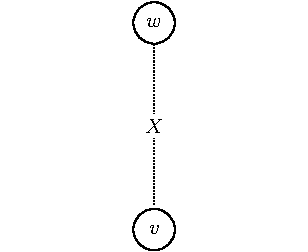
\includegraphics[]{evil_pictures/islands1.pdf}
%\caption{A fairly simple example}
\label{fig:islands1}
}\quad
\subfigure[$w \sqsupseteq_Y \circ\sqsubseteq_X v$\ --\ \newline\ 
``$v$ is $w$'s cousin'']{
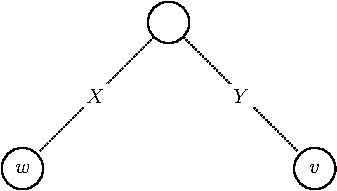
\includegraphics[]{evil_pictures/islands2.pdf}
\label{fig:islands2}
} 
\\
\subfigure[``$v$ is $w$'s second cousin twice removed'']{
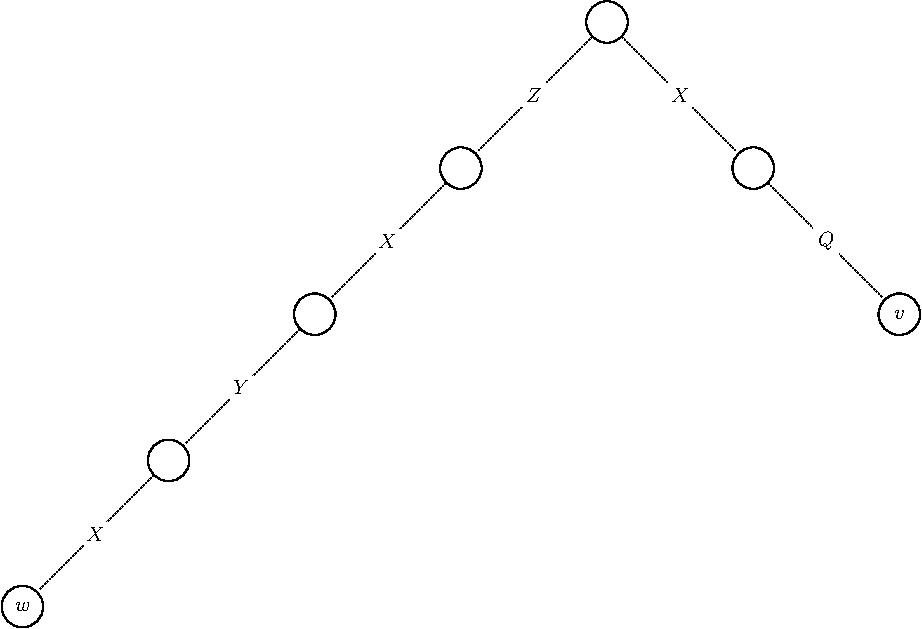
\includegraphics[scale=.5]{evil_pictures/islands3.pdf}
\label{fig:islands3}
}

\caption{Family relationships within columns}
\end{figure}

In many ways, \emph{islands} behave as a single entity;  this is
precisely in accordance with reading \ref{thirdway} above.
We summarize the ways they behave in the following lemma:
%\pagebreak
\begin{lemma}[Island Lemma]\label{island}
The following hold if $\mathbb{M}$ is partly \textsc{EviL}:
\begin{mynum}
	\item\label{island1} For all $w$ we have $w \in \lcorners w\rcorners$
	\item\label{island2} If $w \in \lcorners v\rcorners$ then $\lcorners w\rcorners = \lcorners v\rcorners$
	\item \label{islandR} If $w R_X v$ then for all $u \in \lcorners v\rcorners$
          we have $w R_X u$
\item \label{islandR2} $w R_X v$ if and only if $w R_X \lcorners v
  \rcorners$\footnote{By a minor abuse of notation, 
 $w R_X \lcorners
     v\rcorners$ means that for all $u \in \lcorners v \rcorners$, $w
     R_X u$.
}
	\item \label{islandletters} If $w \in \lcorners v\rcorners$ then $w\in V(p)$ if and only if $v \in V(p)$ for all $p \in \Phi$
\end{mynum}
\end{lemma}
\begin{proof} \ \\
\begin{mynum}
\item This follows since by \ref{ppI} we know that $\sqsubseteq_X$ is
  reflexive.
\item This follows from the general fact that if $w$ is graph-reachable from
  $v$, then $u$ is graph reachable from $w$ if and only if $u$ is
  graph reachable from $v$.
\item Assume that $w R_X v$, and assume that $v \left(\bigcup_{X \in
      \mathcal{A}} \sqsubseteq_X \cup \sqsupseteq_X \right)^\ast u$.
  To show that $w R_X u$, use \ref{ppVI}, that $(\sqsubseteq_Y \circ R_X) = R_X =
    (\sqsupseteq_Y \circ R_X)$, and induction on the path length from
    $v$ to $u$.
\item With \ref{island1}, this is a equivalent to \ref{islandR}.
\item Assume that $w \in \lcorners v \rcorners$, and that $w \in
  V(p)$.  Then we may induct on path length, and use \ref{islandiff}
  to see that $v \in V(p)$.  From \ref{island1} and \ref{island2}
  above, we know that $w \in \lcorners v \rcorners$ implies that $v
  \in \lcorners w \rcorners$, so we can see hat the converse holds
  true too.
\end{mynum}
\end{proof}

\begin{figure}[htbp]
\centering
  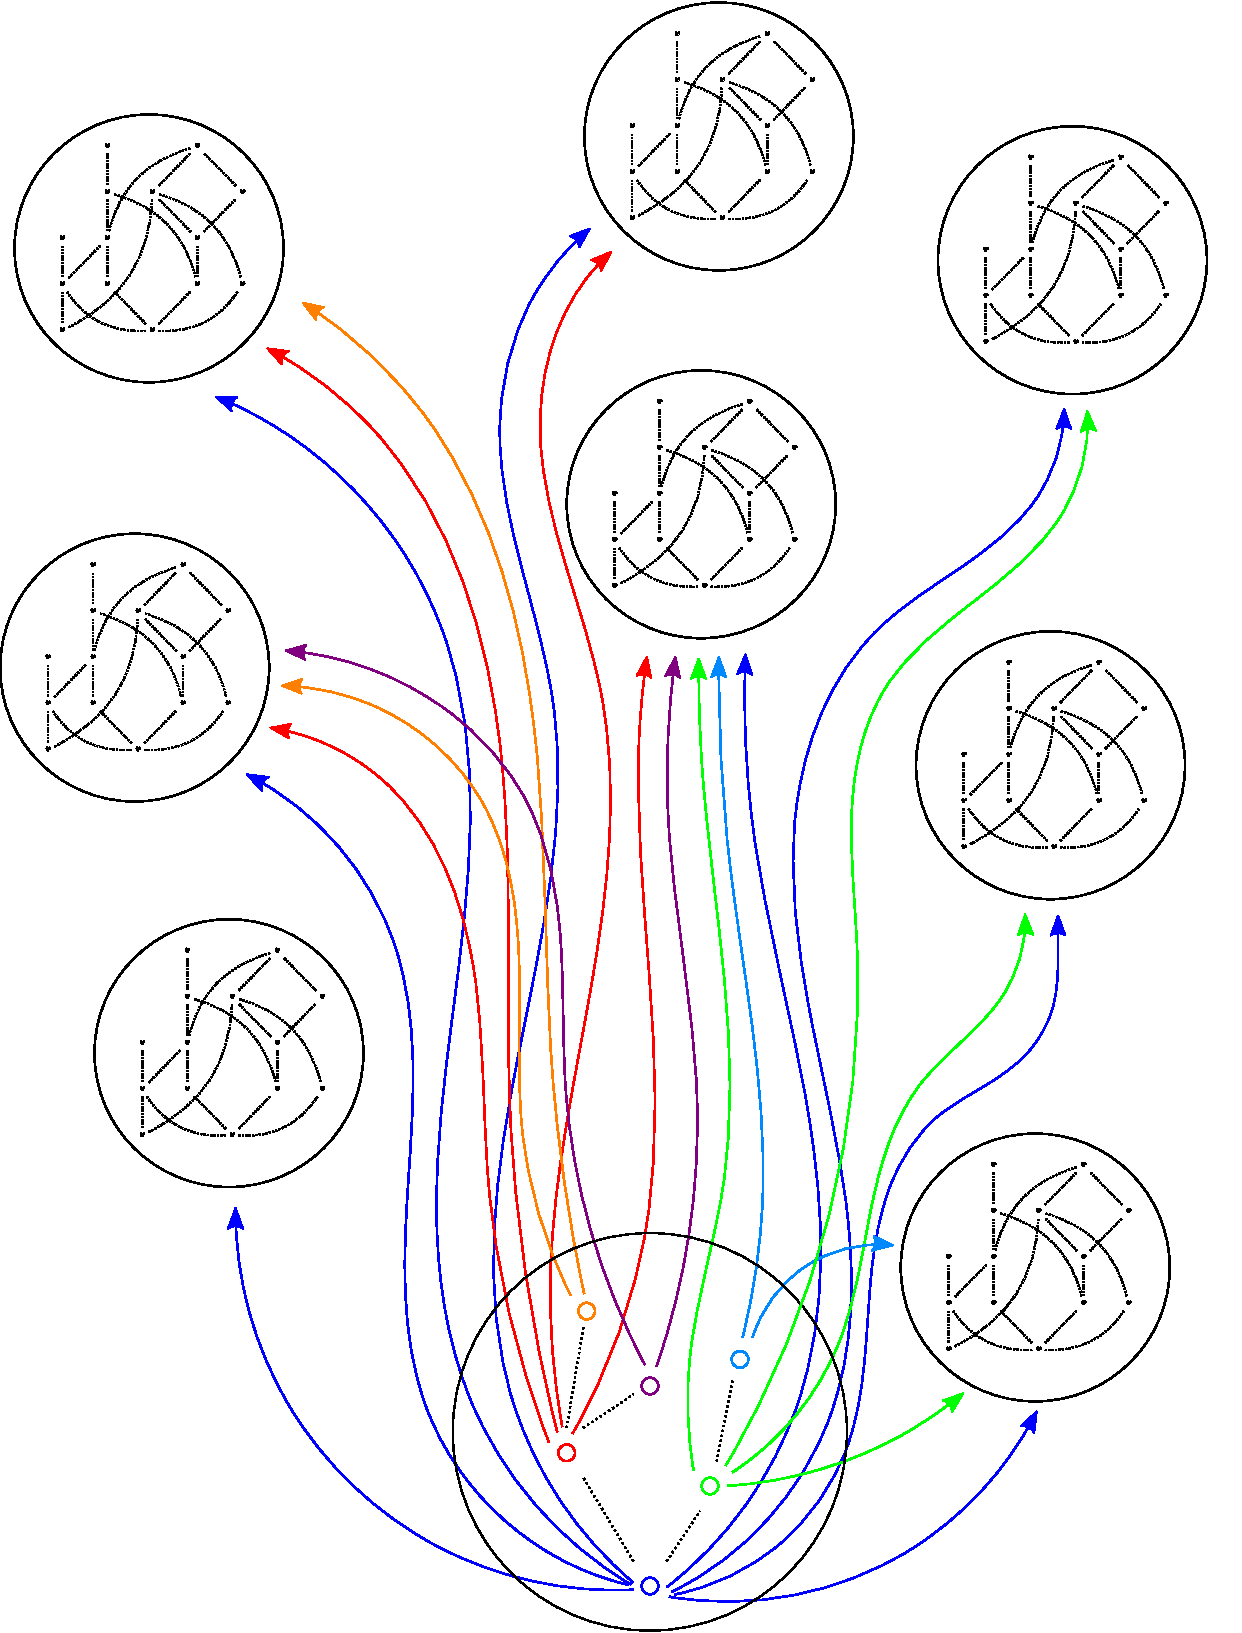
\includegraphics[height=0.9\textheight]{poset/islands.pdf}
%\caption{A fairly simple example}
\caption{The inner functioning of an island and its relations to other islands}
\label{fig:islands}
\end{figure}

\begin{figure}[htbp]
\centering
  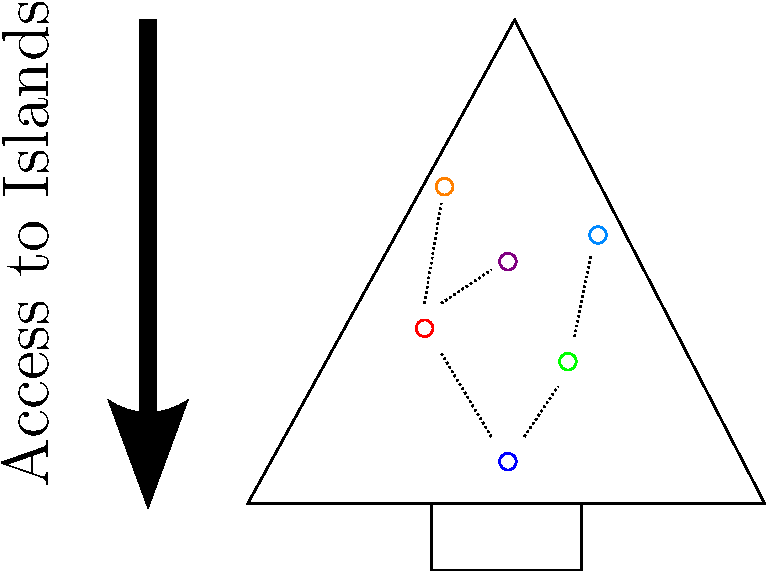
\includegraphics[]{poset/island.pdf}
%\caption{A fairly simple example}
\caption{An island is like a \emph{Christmas tree}}
\label{fig:christmas_island}
\end{figure}

The above lemma asserts that islands are to be thought of as worlds in
of themselves - for they make true the same letters and 
can only be accessed as a unit. Moreover, we know from \ref{ppV}, we
can see in the single agent case that as an agent ``ascends'' in an
island, they can access fewer worlds, which may be equated with
holding more beliefs.  

% The intuitions \ref{ppV} gives us are depicted in
% Fig. \ref{fig:islands}, which shows the inner function of an island in
% the single agent case.  Islands are indicated with circles;
% accessibility arrows associated with $R$ are drawn to entire islands, 
% because as we saw in Lemma \ref{island}, the Island Lemma,  
% islands are accessed as units. Note that worlds and $R$ accessibility 
% arrows are colored in a corresponding manner, to illustrate how 
% accessibility goes up as the agent descends in their island.  

% The differential relationship described above means that, in a sense,
% we may think of an island as like \emph{christmas tree}. This is
% because lower nodes are
% ``wider'' than upper nodes, in the sense that the lower nodes can
% access more worlds.  This situation is depicted in Fig. \ref{fig:island}.

We hope that the above discussion provides some insight into how to
think of islands in an intuitive manner.  In the next section,
we shall show how to leverage the concept of an island to show
how we may translate a finite \textsc{EviL} Kripke structures
witnessing a formula $\phi$ into corresponding \textsc{EviL} models.



%%% Local Variables: 
%%% mode: latex
%%% TeX-master: "evil_philosophy"
%%% End: 


\subsubsection{Translation \& \textsc{Evil} Completeness}
\label{translation}
In this section, we turn to showing that every finite \textsc{EviL}
Kripke structure $\mathbb{M}$ has a corresponding \textsc{EviL} model
$\ipent$ which is an (almost)-homomorphic projection\footnote{Note
  that we shall not provide a formal definition of
  what it means for a map to be (almost)-homomorphic, since we
  consider this concept more intuitive than formal.  Intuitively, two objects
  are \emph{(almost)-homomorphic} when they are homomorphic for all
  intents and purposes.}.  Assuming that $\Phi$ is infinite and $\Psi
\subseteq_{\omega} \Phi$, then we shall show that $\mathbb{M}$
and $\ipent$ agree on the language $\mathcal{L}(\Psi,\mathcal{A})$.  
The method of the proof of this correspondence generalizes the
 elementary argument presented in Proposition
\ref{translation-sketch} from \S\ref{sketch}.  From this
correspondence, we shall obtain a weak completeness theorem for
\textsc{EviL} and its intended semantics.

Recall that in the proof of Proposition \ref{translation-sketch}
 we assumed an infinite store of unused letters, and assigned 
them to worlds in order to control the accessibility in the 
\textsc{EviL} model we constructed.  This was embodied by a function
$p : W \rightarrowtail \Phi \bs L(\phi)$; for each world $w$, $p_w$
was the \emph{name} we assigned to it.  In our construction here, we
shall extend this metaphor, using a generic finite set
$\Psi\subseteq_\omega \Phi$. 

Recall that among the three principle ways we described for thinking
about think about islands, one way to think of $\lcorners w \rcorners$ 
was as $w$'s extended family.  So along with 
\emph{personal names}, we shall also want to assign family 
names or \emph{surnames}.

With these above considerations in mind, we offer the following definition:

\begin{mydef}
Assume the set of letters $\Phi$ is infinite, and fix a finite $\Psi \subseteq_\omega
\Phi$, a finite \textsc{EviL} Kripke
model $\mathbb{M}$
\begin{bul}
\item Let $\Psi$ be a finite set of proposition letters.
% as in the proof of Proposition \ref{translation-sketch} from \S\ref{sketch}
\item Let $$\ang := \{\{w\}, \lcorners w\rcorners \ |\ w
  \in W^{\mathbb{M}}\}$$
That is, $\ang$ is the set of worlds and islands.
\item Let $p: \ang \rightarrowtail \Phi \bs \Psi$ be an
  injection, assigning names to worlds and surnames to
  islands\footnote{Subsequently, we shall abbreviate $p(\{w\})$ as $p_w$ and
    $p(\lcorners w \rcorners)$ as $p_{\lcorners w \rcorners}$}.
\item Let $\kl : W^{\mathbb{M}} \to \powerset \Phi \times
  (\powerset(\mathcal{L}_0(\Phi)))^\mathcal{A}$ be defined such that:
\[ \kl(w) := (\kl_1(w),\kl_2(w)) \]
Where:
\begin{bul}
  \item $\kl_1 : W^{\mathbb{M}} \to \powerset \Phi$ is defined to be:
\[ \kl_1(w) := \{q \in \Psi \ |\ \mathbb{M},w \Vdash q\} \cup
\{p_{\lcorners w\rcorners }\} \]
We may understand $\kl_1$ as providing a propositional valuation to
worlds in $W^{\mathbb{M}}$
\item $\kl_2 : W^{\mathbb{M}} \to \powerset(\mathcal{L}_0(\Phi))$ is defined to be:
\[\kl_2(w) := \prod_{X \in \mathcal{A}} \kl_{2A}(w,X) \cup
\kl_{2B}(w,X) \]
Where:
\begin{bul}
  \item $\kl_{2A} : W^{\mathbb{M}} \times \mathcal{A} \to
    \powerset(\mathcal{L}_0(\Phi))$ is defined to be:
\[ \kl_{2A}(w,X) :=\{ \neg p_{\lcorners v
  \rcorners} \ |\ \neg w R_X v\} \]
 \item $\kl_{2B} : W^{\mathbb{M}} \times \mathcal{A} \to
   \powerset(\mathcal{L}_0(\Phi))$ is defined to be:
\[\kl_{2B}(w,X) := \{ \bot \to p_{v}\ |\ w \sqsupseteq_X v\} \]
\end{bul}
We may understand $\kl_2$ as providing, for each agent, a
corresponding set of propositional formulae.  These formulae constitute their set of basic beliefs, as we originally introduced in
\S\ref{sketch}.

$\kl_{2A}$ and $\kl_{2B}$ each constitute a component that goes into
the basic belief set we assign to a particular agent.
\end{bul}

\item Let $\ipent := \kl[W]$

\end{bul}
\end{mydef}

Certain remarks must be made regarding the above definition.  

For one, note that we are ensured by the axiom of choice that 
$p_w$ is well defined, since by hypothesis we have that 
$W$ is finite, whence
$\powerset W$ is finite and since $\Lambda \subseteq \powerset W$ 
we know that $\Lambda$ is finite as well.  
Since we know that $\Phi$ is infinite then 
$\Phi \bs \Psi$ is infinite as well, and there always
exists an embedding of a finite set into an infinite set.

To be completely explicit about our intentions, $\ipent$ is an 
\textsc{EviL} model we are constructing which shall preserve 
the truth of $\phi$ for all of the worlds in $\mathbb{M}$.  
Our goal is that $\ipent$ should
be an \emph{(almost)-homomorphic projection of
  $\mathbb{M}$ under $\kl$} with respect to a language
$\mathcal{L}(L,\mathcal{A})$, where $L$ is a finite set of letters.  
This is precisely why we have set $\ipent$ to
be the image of $W$ under $\kl$. Permit us to explain what 
``almost homomorphic'' means exactly.

% First, observe that  
% Since the worlds in \textsc{EviL} models are pairs, $\kl$ is broken 
% up into  two operations $\kl_1$ and $\kl_2$ that give each 
% component of each pair.

% The two operations $\kl_1$ and $\kl_2$ deserve some extra motivation,
% since they may be challenging to understand. To see what is going on, 
Recall the definition of $\mho^{\ipent}$ from Definition
\ref{omega-translation} from \S\ref{kripke}. This defines
$\sqsubseteq^{\ipent}$, $\sqsupseteq^{\ipent}$, and $R^{\ipent}$.  To ensure
that $\ipent$ is (almost)-homomorphic to $\mathbb{M}$, 
we shall want to enforce the following relationships:

\begin{align}
q \in \Psi \Longrightarrow (\mathbb{M},w\Vdash q \iff &
\ipent,\kl(w)\VDash q) \label{lettersforce}\\
\mathbb{M},w\Vdash \PP_X \iff & \ipent,\kl(w)\VDash \PP_X \label{Pforce} \\
w \sqsubseteq^\mathbb{M}_X v \iff &  \kl(w) \sqsubseteq^{\ipent}_X
\kl(v) \label{subforce}\\
w \sqsupseteq^\mathbb{M}_X v \iff & \kl(w) \sqsupseteq^{\ipent}_X
\kl(v) \label{supforce}\\
v \in \lcorners w \rcorners^\mathbb{M} \iff &  \kl(v) \in \lcorners \kl(w) \rcorners^{\ipent} \label{islandforce}\\
w R^\mathbb{M}_X v \iff & \kl(w) R^{\ipent}_X
\kl(v) \label{relforce}
\end{align}

So in order for $\ipent$ to ``solve'' the above equations, we have
various logical constraints on our definitions,  which we have used to 
determined the design choices we have made.  We shall show that
$\ipent$ solves the above equations in Lemma \ref{ipentsolution}.

Before we go ahead and prove results about $\ipent$, we shall try to
brush up certain natural questions one may naturally ask about $\ipent$.
\begin{bul}
\item   \emph{Why does $\kl_1(w)$
encode $w$'s surname but not her full name?  That is, why is it that
$p_{\lcorners w\rcorners} \in
\kl_1(w)$ but $p_{w} \nin
\kl_1(w)$?}

Note that in our construction of $\ipent$ we have been trying to enforce
that \eqref{subforce}, \eqref{supforce} and \eqref{islandforce}.
From definition
\ref{omega-translation} from \S\ref{kripke} we know that if $\kl(w) \sqsubseteq^{\ipent}_X \kl(v)$ then
$\kl_1(w) = \kl_1(v)$. Hence we must define $\kl_1$ in such a manner
where if $p_w \in \kl_1(w)$ then $p_w \in \kl_1(v)$.  In fact, since
we are enforcing \eqref{islandforce}, then we know that we cannot encode any information in $\kl_1(w)$ without
putting it into $\kl_1(v)$ for any $v \in \lcorners
w\rcorners^\mathbb{M}$.  However, knowing that we intend to
preserve columns in our construction, we may safely encode 
information about column membership in $\kl_1$, as we have done.
\item \emph{Why does $\kl_2(w)$
encode $\neg p_{\lcorners v \rcorners}$, that is the negation of $v$'s
surname, when $\neg w R_X v$, as opposed to her full name?}  

Recall that we want to enforce that \eqref{relforce}.  We want to make
sure that $\kl(w)$ can ``see'' $\kl(v)$ in all and only those
situations when it is supposed to.  We accomplish this by encoding
surname information into $\kl_1(v)$, and ``blacklisting'' certain
surnames in $\kl_2(w)$ we do not want $w$ to ``see'' using
$R^{\ipent}_X$.  Here we are very consciously exploiting the Lemma
\ref{island}\ref{islandR2}, which asserts if one member of an island is
not accessible to $w$ then nobody on that island is.

\item \emph{Why does $\kl_2(w)$ encode the ``vacuous'' information that $\bot \to p_{v}$ when $w \sqsupseteq_X v$?}
In order to enforce \eqref{subforce} and \eqref{supforce}, we need to
encode information regarding $\sqsubseteq_X^\mathbb{M}$ and $\sqsupseteq_X^\mathbb{M}$
somewhere.  We cannot encode this information
in $\kl_1$, for the reason that it can only safely encode information
at the island level using surnames.  
Hence we must encode this information in $\kl_2$; 
it is for this reason that we have chosen to include 
$\bot \to p_{v} \in \kl_{2B}(w,X)$.

However, we do not want the information we encode in $\kl_{2B}(w,X)$ to
interfere with $R^{\ipent}_X$, so one way to ensure that ``harmless''
information is encoded is to use tautologies, as we have done.
\end{bul}

Hopefully the reader has some intuition about the engineering choices
we made in the construction of $\ipent$.  We now turn to proving
that $\ipent$ satisfies our design criteria.

\begin{lemma}\label{ipentsolution}
Provided that $\mathbb{M}$ is \textsc{EviL}, our definition of
$\ipent$ suffices \eqref{lettersforce} through \eqref{relforce}.
\end{lemma}
\begin{proof} \ 
  \begin{bul}
    \item \eqref{lettersforce} 
\begin{align*}
q \in \Psi \Longrightarrow (\mathbb{M},w\Vdash q \iff &
\ipent,\kl(w)\VDash q)
\end{align*}
Let $q \in \Psi $.   We have two directions we must reason:
\begin{description}
\item[$\Longrightarrow$]
First assume that $\mathbb{M},w\Vdash q$.  We know that 
\begin{align*}
\ipent,\kl(w)\VDash q & \iff q \in \kl_1(w) \\
& \iff q \in \{q \in \Psi \ |\ \mathbb{M},w \Vdash q\} \cup
\{p_{\lcorners w\rcorners }\}
\end{align*}
Hence $\ipent,\kl(w)\VDash q$ as desired.

\item[$\Longleftarrow$]
Assume that $\ipent,\kl(w)\VDash q$, we to show $\mathbb{M},w\Vdash
q$. By our assumption we have either $q \in \{q \in
L \ |\ \mathbb{M},w \Vdash q\}$ or $q \in \{p_{\lcorners
  w\rcorners }\}$.  In the former case we are done, and the latter
case is impossible since $p_{\lcorners w \rcorners} \in \Phi \bs \Psi $ 
by definition, hence it is impossible for $q \in
\{p_{\lcorners w\rcorners }\}$ by hypothesis.
\end{description}

\item \eqref{Pforce} 
\begin{align*}
\mathbb{M},w\Vdash \PP_X \iff & \ipent,\kl(w)\VDash \PP_X
\end{align*}
Since $\mathbb{M}$ is \textsc{EviL}, and
      $\ipent, \kl(w) \VDash \PP_X$ if and only if $\kl(w)
      R^{\ipent}_X \kl(w)$, by virtue of property 
      \ref{pVI} of \textsc{EviL} Kripke models it suffices 
     to prove \eqref{relforce} below.


\item \eqref{subforce}
\begin{align*}
w \sqsubseteq^\mathbb{M}_X v \iff &  \kl(w) \sqsubseteq^{\ipent}_X
\kl(v)
\end{align*}  
We have two directions to show:
\begin{description}
\item[$\Longrightarrow$] Assume that $w \sqsubseteq^\mathbb{M}_X v$.
  To ensure $\kl(w) \sqsubseteq^{\ipent}_X \kl(v)$ we need to ensure
  two things:
\begin{myroman}
\item $\kl_1(w) = \kl_1(v)$ --  In order for this to be the case, we
  must have: 
\[ \underbrace{\{q \in \Psi \ |\ \mathbb{M},w \Vdash q\}}_A \cup
\underbrace{\{p_{\lcorners w\rcorners }\}}_B = \underbrace{\{q \in \Psi \ |\ \mathbb{M},v \Vdash q\}}_C \cup
\underbrace{\{p_{\lcorners v\rcorners }\}}_D\]
Note that by hypothesis, $w$ and $v$ are on the same island, which
means that $B = D$.   Since if two worlds in an \textsc{Evil} model
are on the same island,
%  (ie. $w \sqsubseteq_X^\mathbb{M} v
% \Longrightarrow \lcorners w \rcorners = \lcorners v \rcorners$) 
then by the Island Lemma they make the same proposition letters true, hence $A =
C$, which suffices.
\item $(\kl_2(w))_X \subseteq  (\kl_2(v))_X$ --  Since $(\kl_2(u))_X =
  \kl_{2A}(u,X) \cup \kl_{2B}(u,X)$, it suffices to show that
  $\kl_{2A}(w,X) \subseteq \kl_{2A}(v,X)$ and $\kl_{2B}(w,X) \subseteq
  \kl_{2B}(v,X)$:
\begin{bul}
\item $\kl_{2A}(w,X) \subseteq \kl_{2A}(v,X)$ --  Assume that $x \in
  \kl_{2A}(w,X)$.  Then $x = \neg p_{\lcorners u\rcorners}$ for some $u \in W$
  where $\neg w R_X^{\mathbb{M}} u$. It suffices to show that $\neg v R_X^{\mathbb{M}} u$.  

Suppose towards a contradiction that $v R_X^{\mathbb{M}} u$, 
then by hypothesis we have that $w
  R_X^{\mathbb{M}} \circ \sqsubseteq_X^{\mathbb{M}} u$.  However, we know that since
  $\mathbb{M}$ is \textsc{EviL} then by \ref{pV} we have that $R_X^{\mathbb{M}}
  \circ \sqsubseteq_X^{\mathbb{M}} \subseteq R_X^{\mathbb{M}}$, which
  means that $w R_X^{\mathbb{M}} u$ after all. $\lightning$ 
\item $\kl_{2B}(w,X) \subseteq \kl_{2B}(v,X)$ --  Assume that $x \in
  \kl_{2B}(w,X)$, then $x = \bot \to p_u$ for some $u$ such that $u
  \sqsubseteq_X^{\mathbb{M}} w$.  Then by transitivity we have that $u
  \sqsubseteq_X^{\mathbb{M}} v$, which means that $\bot \to p_u \in \kl_{2B}(v,X)$  as desired.
\end{bul}  
\end{myroman}

\item[$\Longleftarrow$]  Assume that $\kl(w) \sqsubseteq_X^{\ipent}
  \kl(v)$.  We know that since $\mathbb{M}$ is \textsc{EviL} then
  $\sqsubseteq^\mathbb{M}_X$ is reflexive, so $w \sqsubseteq_X^\mathbb{M} w$, whence $\bot \to
  p_w \in \kl_{2B}(w)$.  Thus $\bot \to p_w \in (\kl_2(v))_X$, which means
  that either $\bot \to p_w \in \kl_{2A}(v,X)$ or $\bot \to p_w \in
  \kl_{2B}(v,X)$.  We can see that $\bot \to p_w \neq \neg
  p_{\lcorners u\rcorners}$ for all $u$ since these formulae are of different forms, so it must be that $\bot \to p_w \in \kl_{2B}(v)$.  This means that $w
  \sqsubseteq_X^\mathbb{M} v$, as desired.
\end{description}
\item \eqref{supforce} 
\begin{align*}
w \sqsupseteq^\mathbb{M}_X v \iff & 
\kl(w) \sqsupseteq^{\ipent}_X \kl(v) \\
\end{align*}

This
  follows from \eqref{subforce} and the fact that both $\mathbb{M}$ and $\ipent$ are
  \textsc{EviL}, hence $x \sqsubseteq_X y \iff y \sqsupseteq_X x$ for
  both structures.

\item \eqref{islandforce}  
\begin{align*}
v \in \lcorners w \rcorners^\mathbb{M} \iff &  \kl(v) \in \lcorners \kl(w) \rcorners^{\ipent}
\end{align*}
The fact that islands in both structures
  correspond follows from the correspondences between $\sqsubseteq_X$ and
  $\sqsupseteq_X$, as we already saw in \eqref{subforce} and \eqref{supforce}.
\item\eqref{relforce} 
\begin{align*}
w R^\mathbb{M}_X v \iff & \kl(w) R^{\ipent}_X \kl(v)
\end{align*}
\begin{description}
\item[$\Longrightarrow$]
First assume that $w R^\mathbb{M}_X v$, we want to show $\kl(w) R^{\ipent}_X
\kl(v)$.  
This means that we must show $\kl_1(v) \models
(\kl_2(w))_X$.  
Since $(\kl_2(w))_X = \kl_{2A}(w,X) \cup
\kl_{2B}(w,X)$, we have two steps:
\begin{description}
  \item[$\kl_1(v) \models \kl_{2A}(w,X)$ --]  Assume that $\kl_1(v)
    \nmodels \kl_{2A}(w,X)$, then it must be that there is some $u\in
    W^\mathbb{M}$ where $p_{\lcorners u\rcorners} \in
    \kl_1(u)$ and $\neg p_{\lcorners u\rcorners} \in \kl_{2A}(w)$,
    which means that $\neg w R^{\mathbb{M}}_X u$.
    Since $p_{\lcorners u\rcorners} \nin L(\Phi)$ it must be that
    $p_{\lcorners u\rcorners} = p_{\lcorners v\rcorners}$, hence $\lcorners u \rcorners = \lcorners v \rcorners$. Then by the
     Island Lemma we have $\neg w R^{\mathbb{M}}_X v$ after
    all. $\lightning$
  \item[$\kl_1(v) \models \kl_{2B}(w,X)$ --]  Simply note that
    everything in $\kl_{2B}(w,X)$ is a tautology, by construction, 
    so this step follows vacuously.
\end{description}
\item[$\Longleftarrow$]  Assume $\kl(w) R^{\ipent}_X \kl(v)$, in other words
  $\kl_1(v) \models (\kl(w))_X$.  We shall show $w R^\mathbb{M}_X v$.
  So suppose to the contrary that $\neg w R^\mathbb{M}_X v$, then
  $\neg p_{\lcorners v\rcorners} \in \kl_{2A}(w)$.  However we know
  that $p_{\lcorners
    v\rcorners} \in \kl_1(v)$, hence $\kl_1 \models p_{\lcorners
    v\rcorners}$, which means that $\kl_1(v) \nmodels (\kl(w))_X$,
  which contradicts our assumption. $\lightning$
\end{description}
\end{bul}
\end{proof}

Having established that $\ipent$ is indeed (almost)-homomorphic to
$\mathbb{M}$, we may use this to show that $\mathbb{M}$ and $\ipent$
are logically the same over $\mathcal{L}(\Psi, \mathcal{A})$.

\begin{lemma}[\textsc{EviL} Translation]\label{translation-lemma}
Let $\mathbb{M}$ be an \textsc{EviL} Kripke structure.  For any
formula $\phi \in \mathcal{L}(\Psi)$, and any $w \in W$, we have
\[ \mathbb{M},w \Vdash \phi \iff \ipent, \kl(w) \VDash \phi \]
\end{lemma}
\begin{proof}
Using induction, and Lemma \ref{ipentsolution}, the result follows
from the fact that $\ipent$ and $\mathbb{M}$ correspond in all of the
ways relevant to $\mathcal{L}(\Psi,\mathcal{A})$. 
\end{proof}

Hence, from the above, we may prove a central result of \textsc{EviL}:

\begin{theorem}[\textsc{EviL} Soundness and Weak Completeness]
\label{conc-evil-completeness}
\[ \vdash_{\textsc{EviL}} \phi \iff \VDash \phi \]
\end{theorem}
\begin{proof}
Soundness is trivial, so we shall only prove completeness.

Assume that $\nvdash \phi$. We know from Theorem
\ref{abst-finite-completeness} that there is a finite $\mathbb{M}$
such that $\mathbb{M},w \nVdash \phi$ for some $w \in W$.

Now let $\Psi = L(\phi)$, where $L(\phi)$ is the letters that occur in
$\phi$, just as we originally defined in the proof of Proposition \ref{translation-sketch} 
from \S\ref{sketch}.  Since 
$\phi \in \mathcal{L}(L(\phi),\mathcal{A})$, from lemma
\ref{translation-lemma} we have that $\ipent, \kl(w) \nVDash \phi$.
Then evidently $\ipent$ is our desired counter model, hence we have
the theorem.
\end{proof}

With this, we may conclude the proof of completeness of \textsc{EviL}.
%%% Local Variables: 
%%% mode: latex
%%% TeX-master: "evil_philosophy"
%%% End: 

% \subsubsection{\textsc{EviL} Completeness}\label{skarmy-of-darkness} 
% With the results of the previous sections provided, we may now show
that \textsc{EviL} is complete for \textsc{EviL} models.

\begin{theorem}
If $\nvdash \phi$ then there is some model $\mathfrak{M}$ and some $(a,A) \in \mathfrak{M}$ such that $\mathfrak{M},(a,A) \nmodels \phi$ 
\end{theorem}
\begin{proof}
	Assume $\nvdash \phi$, then by Lemmas \ref{truth} and \ref{partly} we have some partly \textsc{EviL} Kripke 
	structure and world such that $\mathbb{A},a \nVdash \phi$.  By Lemma \ref{bisimulation} we have that there is a 
	completely \textsc{EviL} Kripke structure $\mathbb{B}$ such that $\mathbb{A}\ \underline{\IFF}{}\ \mathbb{B}$, thus there is some world $b$ such that $\mathbb{B},b \nVdash \phi$.  
	Finally by Lemma \ref{translation-lemma} we have that there's a model $\mathfrak{C}$ in \textsc{EviL} semantics and a pair $(c,C) \in \mathfrak{C}$ such that $\mathfrak{C},(c,C) \nmodels \phi$.
\end{proof}

%%% Local Variables: 
%%% mode: latex
%%% TeX-master: "evil_philosophy"
%%% End: 


\subsubsection{Taking Stock II}\label{taking-stockII}
In this section, we take stock of what we have illustrated so far in
our investigations into the completeness of \textsc{EviL}.  We discuss
how the nature of the abstract semantics for \textsc{EviL} in
relationship to its concrete semantics, and we view this relationship
from a wider mathematical perspective.

We shall begin by substantiating the relationship we established in
\S\ref{taking-stock}, which we expressed in \eqref{relationship}.

\begin{lemma}\label{coincide} For $\Gamma\subseteq_\omega \mathcal{L}(\Phi, \mathcal{A})$ and infinite $\Phi$:
\[
\Gamma \Vdash_{\textsc{EviL}} \phi \iff \Gamma \VDash \phi
\]
\end{lemma}
\begin{proof}
We may observe that since $\Gamma$ is finite, then by classical logic
and our previous completeness theorems we have the following chain of reasoning:
\begin{align*}
  \Gamma \Vdash_{\textsc{EviL}} \phi & \iff  \Vdash_{\textsc{EviL}} \bigwedge \Gamma
  \to \phi \\
   & \iff \vdash_{\textsc{EviL}} \bigwedge \Gamma
  \to \phi \\
   & \iff \VDash \bigwedge \Gamma
  \to \phi \\
   & \iff  \Gamma \VDash \phi
\end{align*}
\end{proof}

As a further remark, we feel the need to discuss the nature of the
relationship between the \emph{concrete} and \emph{abstract} semantics
that \textsc{EviL} exhibits.  We began with \textsc{EviL} models,
which were intended to model intuitions we had regarding the nature of
epistemology.  In so doing, we used the language of traditional 
epistemic logic, even though we modified the semantics heavily.  We
found this gave rise to relational models that are the traditional
object of study of modal logic, however we found that while we could
abstract to traditional Kripke structures, this was not symmetric --
we could not abstract back.

We argue that this particular relationship is commonplace in
mathematics.  For instance, it is natural to think of the integers as
a concrete object.  After all, every mathematics student at some point
learns Kronicker's legendary mantra ``God created the integers, all
else is the creation of man'' \cite[pg. 477]{bell_men_1986}.
However, it is by these concrete origins, we may recognize the
integers as a concrete Noetherian ring, and carry on understanding
mathematics on a more abstract and general fashion.
%   Indeed, it is by understanding
% the integers that the theory of Noetherian rings proceeds.
  For instance, the fact that every ideal in a Noetherian ring is equal to a finite
intersection of primary ideals is a pure abstraction of 
Euclid's prime decomposition theorem\cite[Lemmas 7.11 and 7.12,
pg. 83]{atiyah_introduction_1994}.  This is part of the character of
mathematics; abstraction is guided by intuition drawn from more
concrete objects.  In  the same manner we may regard \emph{Stone
Representation Theorem} as an infinitary abstraction of
\emph{Birkoff's Theorem} \cite[chapters 11 and 5,
respectively]{davey_introduction_2002}, and the \emph{Yoneda Lemma} as
an abstraction of Cayley's
theorem \cite[chapters 4 and 1, respectively]{smith_post-modern_1999}.

Despite the order of presentation given here, we should make things
clear: we did not derive the abstract completeness theorem in
\S\ref{abstraction} until we were convinced that \textsc{EviL} Kripke
structures generalized our concrete structures.  The process by which
\textsc{EviL} was developed involved finding the results in
\S\ref{small-model} first, and letting the defining properties of
concrete \textsc{Evil} models define the logic.  
Abstract completeness was an afterthought.  Of course, just as in the
case of complex analysis and trigonometry, our abstract formalism
is far easier to manipulate than our original \textsc{EviL} models.
Moreover, since the abstract completeness theorem is far simpler than
the concrete completeness theorem, our presentation has followed suit.

\textsc{EviL} Kripke structures really are abstract
idealizations of concrete \textsc{EviL} models, as we have
illustrated.  This puts us in a powerful position. 
On the one hand, we have concrete semantics by
which we may sharpen our intuition. On the other hand, we 
have well behaved abstract semantics which faithfully provide an 
idealized domain for us to carry out formal work with relative ease.
We feel the situation is analogous to the one in \emph{complex analysis}, where
the easiest way to prove trigonometric theorems is to employ complex
idealizations such as \emph{Euler's Formula} (the reader will recall this is
the assertion $e^{i \theta} = \cos \theta + i \sin \theta$).  Perhaps
more appropriately, we can think of the space of \textsc{EviL}
Kripke structures as a \emph{compactification}, in a sense, of the
concrete \textsc{EviL} models, since the logic is indeed compact over
the Kripke structure abstraction.

The subsequent sections shall go on to illustrate how we may use
abstract Kripke semantics to easily understand properties of
\textsc{EviL}, and show that we may use the correspondence exhibited
in \eqref{relationship} to transfer these results to \textsc{EviL} models.

%%% Local Variables: 
%%% mode: latex
%%% TeX-master: "evil_philosophy"
%%% End: 


\subsubsection{Subsystems of \textsc{EviL}}\label{subsystems}
In this section, we shall investigate two subsystems of
single agent \textsc{EviL}.

We first consider the following two fragments of the main grammar.
\begin{definition}
Define $\mathcal{L}^\boxminus (\Phi)$ as the fragment:
\[ \phi \ {::=} \  p \in \Phi \  | \  \phi
   \rightarrow \psi \  | \  \bot \  |
   \  \Box \phi \  | \  \boxminus \phi
%   \  | \  \boxplus \phi
 \  | \ 
   \circlearrowleft \]

Define $\mathcal{L}^\boxplus (\Phi)$ as the fragment:
%Define $\mathcal{L}^\boxminus (\Phi, \mathcal{A})$ as the fragment:
\[ \phi \ {::=} \  p \in \Phi \  | \  \phi
   \rightarrow \psi \  | \  \bot \  |
   \  \Box \phi 
%\  | \  \boxminus \phi
   \  | \  \boxplus \phi
 \  | \ 
   \circlearrowleft \]
\end{definition}

It is natural to wonder about \textsc{EviL} restricted to thee two
fragments.  After all, while ideas from Cartesian skepticism
naturally leads one to think about $\mathcal{L}^\boxminus(\Phi)$, as we saw in \S\ref{Descartes}, 
it is harder to motivate $\mathcal{L}^\boxplus (\Phi)$.
However, we regard each fragment as worthy of study in its own right.

Table \ref{table:axiomsII} gives the axioms systems for the two
fragments in question.  The system corresponding to the
$\mathcal{L}^\BM$ fragment is referred to as \textsc{EviL}$^\BM$, and
similarly the fragment corresponding to the $\mathcal{L}^\BP$ fragment
is referred to as \textsc{EviL}$^\BP$.

% For now, we shall observe that \textsc{EviL} extends \textsc{EviL}$^\BM$ and \textsc{EviL}$^\BP$.  In \S\ref{conservative-extension} we shall make this precise. 
\begin{table}
\begin{minipage}[b]{0.5\linewidth}
\centering
%\newcounter{rownum}
\setcounter{rownum}{0}
%\newcounter{rownum2}
\setcounter{rownum2}{0}
\begin{tabular}{|ll|}
\hline
  (\addtocounter{rownum}{1}\arabic{rownum})&$ \vdash \phi \rightarrow \psi \rightarrow \phi$\\
  (\addtocounter{rownum}{1}\arabic{rownum})&$ \vdash (\phi \rightarrow \psi \rightarrow \chi) \rightarrow (\phi
  \rightarrow \psi) \rightarrow \phi \rightarrow \chi$\\
  (\addtocounter{rownum}{1}\arabic{rownum})&$ \vdash (\neg \phi \rightarrow \neg \psi) \rightarrow \psi \rightarrow
  \phi$\\
  (\addtocounter{rownum}{1}\arabic{rownum})&$ \vdash \boxminus_X \phi \rightarrow \phi$\\
  (\addtocounter{rownum}{1}\arabic{rownum})&$ \vdash \boxminus_X \phi \rightarrow \boxminus_X \boxminus_X \phi$\\
  (\addtocounter{rownum}{1}\arabic{rownum})&$ \vdash p \rightarrow \boxminus_X p$\\
  (\addtocounter{rownum}{1}\arabic{rownum})&$ \vdash \neg p \rightarrow \boxminus_X \neg p$\\
  (\addtocounter{rownum}{1}\arabic{rownum})&$ \vdash \diamondsuit_X \phi \rightarrow \boxminus_X \diamondsuit_X \phi$\\
  (\addtocounter{rownum}{1}\arabic{rownum})&$ \vdash \Box_X \phi \rightarrow \Box_X \boxminus_Y \phi$\\
  (\addtocounter{rownum}{1}\arabic{rownum})&$ \vdash \phi \rightarrow \boxminus_X (\circlearrowleft_X \rightarrow
  \diamondsuit_X \phi)$\\
  (\addtocounter{rownum}{1}\arabic{rownum})&$ \vdash \circlearrowleft_X \rightarrow \boxminus_X \circlearrowleft_X$\\
  (\addtocounter{rownum}{1}\arabic{rownum})&$ \vdash \Box_X (\phi \rightarrow \psi) \rightarrow \Box_X \phi \rightarrow
  \Box_X \psi$\\
  (\addtocounter{rownum}{1}\arabic{rownum})&$ \vdash \boxminus_X (\phi \rightarrow \psi) \rightarrow \boxminus_X \phi
  \rightarrow \boxminus_X \psi$\\
(\addtocounter{rownum2}{1}\Roman{rownum2}) & 
 $\AxiomC{$\vdash \phi \to \psi$}
\AxiomC{$\vdash \phi$}
\BinaryInfC{$\vdash \psi$}
\DisplayProof$ \\ %& Modus Ponens\\[10pt]
(\addtocounter{rownum2}{1}\Roman{rownum2}) & 
 $\AxiomC{$\vdash \phi$}
\UnaryInfC{$\vdash \Box_X \phi$}
\DisplayProof$ \\ %& \multirow{3}{8.5cm}{Variations on necessitation}\\
(\addtocounter{rownum2}{1}\Roman{rownum2}) & 
 $\AxiomC{$\vdash \phi$}
\UnaryInfC{$\vdash \BB_X \phi$}
\DisplayProof$   \\
% (\addtocounter{rownum2}{1}\Roman{rownum2}) &
%  $\AxiomC{$\vdash \phi$}
% \UnaryInfC{$\vdash \BBI_X \phi$}
% \DisplayProof$  \\% [10pt]
\hline
\end{tabular}
\end{minipage}
\hspace{0.5cm}
\begin{minipage}[b]{0.5\linewidth}
 \centering
%\newcounter{rownum}
\setcounter{rownum}{0}
%\newcounter{rownum2}
\setcounter{rownum2}{0}
\begin{tabular}{|ll|}
\hline
  (\addtocounter{rownum}{1}\arabic{rownum})&$ \vdash \phi \rightarrow \psi \rightarrow \phi$\\
  (\addtocounter{rownum}{1}\arabic{rownum})&$ \vdash (\phi \rightarrow \psi \rightarrow \chi) \rightarrow (\phi
  \rightarrow \psi) \rightarrow \phi \rightarrow \chi$\\
  (\addtocounter{rownum}{1}\arabic{rownum})&$ \vdash (\neg \phi \rightarrow \neg \psi) \rightarrow \psi \rightarrow
  \phi$\\
  (\addtocounter{rownum}{1}\arabic{rownum})&$ \vdash \boxplus_X \phi \rightarrow \phi$\\
  (\addtocounter{rownum}{1}\arabic{rownum})&$ \vdash \boxplus_X \phi \rightarrow \boxplus_X \boxplus_X \phi$\\
  (\addtocounter{rownum}{1}\arabic{rownum})&$ \vdash p \rightarrow \boxplus_X p$\\
  (\addtocounter{rownum}{1}\arabic{rownum})&$ \vdash \neg p \rightarrow \boxplus_X \neg p$\\
  (\addtocounter{rownum}{1}\arabic{rownum})&$ \vdash \Box_X \phi \rightarrow \boxplus_X \Box_X \phi$\\
  (\addtocounter{rownum}{1}\arabic{rownum})&$ \vdash \Box_X \phi \rightarrow \Box_X \boxplus_Y \phi$\\
  (\addtocounter{rownum}{1}\arabic{rownum})&$ \vdash \phi \rightarrow \boxplus_X (\circlearrowleft_X \rightarrow
  \diamondsuit_X \phi)$\\
  (\addtocounter{rownum}{1}\arabic{rownum})&$ \vdash \neg \circlearrowleft_X \rightarrow \boxplus_X \neg
  \circlearrowleft_X$\\
  (\addtocounter{rownum}{1}\arabic{rownum})&$ \vdash \Box_X (\phi \rightarrow \psi) \rightarrow \Box_X \phi \rightarrow
  \Box_X \psi$\\
  (\addtocounter{rownum}{1}\arabic{rownum})&$ \vdash \boxplus_X (\phi \rightarrow \psi) \rightarrow \boxplus_X \phi
  \rightarrow \boxplus_X \psi$\\
(\addtocounter{rownum2}{1}\Roman{rownum2}) & 
 $\AxiomC{$\vdash \phi \to \psi$}
\AxiomC{$\vdash \phi$}
\BinaryInfC{$\vdash \psi$}
\DisplayProof$ \\ %& Modus Ponens\\[10pt]
(\addtocounter{rownum2}{1}\Roman{rownum2}) & 
 $\AxiomC{$\vdash \phi$}
\UnaryInfC{$\vdash \Box_X \phi$}
\DisplayProof$ \\ %& \multirow{3}{8.5cm}{Variations on necessitation}\\
% (\addtocounter{rownum2}{1}\Roman{rownum2}) & 
%  $\AxiomC{$\vdash \phi$}
% \UnaryInfC{$\vdash \BB_X \phi$}
% \DisplayProof$   \\
(\addtocounter{rownum2}{1}\Roman{rownum2}) &
 $\AxiomC{$\vdash \phi$}
\UnaryInfC{$\vdash \BBI_X \phi$}
\DisplayProof$  \\% [10pt]
\hline
\end{tabular}
\end{minipage}
\caption{Axiom system \textsc{EviL}$^\BM$ and \textsc{EviL}$^\BP$ respectively}
\label{table:axiomsII}
\end{table}

From these axioms, we shall define two sorts of \emph{\textsc{EviL}} models the correspond to the properties defined by
the above axiom systems.

% One should note that \textsc{EviL}$^\BM$ only induces properties on
% $\sqsupseteq$, and similarly \textsc{EviL}$^\BP$ only induces
% properties on $\sqsubseteq$. In each case, if either
% $\sqsubseteq$ or $\sqsupseteq$ has no defining axioms given by
% the logic then we shall simply assume that it is the inverse of its
% dual. 

% when we are restricting ourselves
% to thinking about $\mathcal{L}^\BM$, we 
\pagebreak

\begin{definition}The following properties specify 
\textbf{$\BM$\textsc{EviL}} and \textbf{$\BP$\textsc{EviL}} Kripke structures:

\begin{minipage}[b]{0.5\linewidth}
\begin{center}
\textbf{$\BM$\textsc{EviL}}
\end{center}
  \begin{enumerate}[label=\textup{(\emph{\Roman*})$^\BM$}, topsep=0.0in, parsep=0.075in]
    \item \label{MpI} $\sqsupseteq$ is reflexive
    \item \label{Mptrans} $\sqsupseteq$ is transitive 
    \item \label{Mpantisym} $\sqsupseteq$ is anti-symmetric
    \item \label{Mpreverse} $w \sqsupseteq v$ if and only if $v
    \sqsubseteq w$
   \item \label{Mislandiff} If $w \sqsupseteq v$ then ($w \in V (p)$ if and only if $v \in V (p)$)
     \item \label{MpV} $(R^{} \circ \sqsubseteq^{}) \subseteq
    R^{} \subseteq (R^{} \circ \sqsupseteq^{})$
     \item \label{MpVI} $(\sqsupseteq^{} \circ R^{}) \subseteq
R^{} \subseteq
(\sqsubseteq^{} \circ R^{})$
     \item\label{MpVII} 
If $w \sqsupseteq v$ and $v \in P$ then $v R w$

    \item\label{MpIX} If $w \in P$ and $w \sqsupseteq v$ then $v
     \in P$
  \end{enumerate}
\end{minipage}
\hspace{0.5cm}
\begin{minipage}[b]{0.5\linewidth}
\begin{center}
\textbf{$\BP$\textsc{EviL}}
\end{center}
  \begin{enumerate}[label=\textup{(\emph{\Roman*})$^\BP$}, topsep=0.0in, parsep=0.075in]
    \item \label{PpI} $\sqsubseteq$ is reflexive
    \item \label{Pptrans} $\sqsubseteq$ is transitive 
    \item \label{Ppantisym} $\sqsubseteq$ is anti-symmetric
    \item \label{Ppreverse} $w \sqsubseteq v$ if and only if $v \sqsupseteq w$
   \item \label{Pislandiff} If $w \sqsubseteq v$ then ($w \in V (p)$ if and only if $v \in V (p)$)
     \item \label{PpV}  $(R^{} \circ \sqsubseteq^{}) \subseteq
    R^{} \subseteq (R^{} \circ \sqsupseteq^{})$
     \item \label{PpVI} $(\sqsubseteq^{} \circ R^{}) \subseteq
 R^{} \subseteq (\sqsupseteq^{} \circ R^{})$
     \item\label{PpVII} If $w \sqsubseteq v$ and $v \in P$ then $v
       R w$

    \item\label{PpIX} If $w \nin P$ and $w \sqsubseteq v$ then $v
     \nin P$
  \end{enumerate}
\end{minipage}
\end{definition}

Exactly as in the case of the \textsc{EviL} Kripke structures we
introduced in \S\ref{kripke}, we may naturally visualize certain
properties in commutative diagrams:
\begin{bul}
%\item Properties \ref{MpV} and \ref{PpV} are depicted in
%Fig. \ref{fig:dupcommut1}
\item  Property \ref{MpVI} is depicted as
Fig. \ref{fig:dupcommut2}, which is the same as Fig. \ref{fig:commut2}
\item  Property \ref{PpVI} is depicted as
Fig. \ref{fig:dupcommut2}, which is the same as Fig. \ref{fig:commut3}
\end{bul}

\begin{figure}[ht]
\centering
% \subfigure[--\ \ref{MpV} \& \ref{PpV}\ -- ]{
%   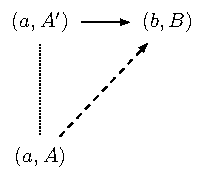
\includegraphics[]{commutative/commutative1.pdf}
% %\caption{A fairly simple example}
% \label{fig:dupcommut1}
% }
% \hspace{1cm}
\subfigure[--\ \ref{MpVI}\ -- ]{
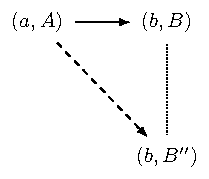
\includegraphics[]{commutative/commutative3.pdf}
\label{fig:dupcommut2}
}
\hspace{1cm}
\subfigure[--\ \ref{PpVI}\ --]{
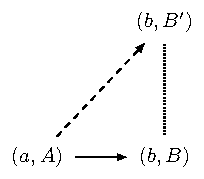
\includegraphics[]{commutative/commutative2.pdf}
\label{fig:dupcommut3}
}
\caption{Visualizations of the relationships in Proposition \ref{evil_models}}
\end{figure}

We may recall that the commutative diagrams depicted split
the original \textsc{EviL} property \ref{pV};  this is not coincidental.
By elementary reasoning we may observe that every 
partly \textsc{EviL} Kripke structure 
(and hence, every \textsc{EviL} Kripke structure) is  
both $\BM$\textsc{EviL} and $\BP$\textsc{EviL}.  In fact, the logical differences between partly
\textsc{EviL}, $\BM$\textsc{EviL}, and $\BP$\textsc{EviL} properties respectively may be summarized as follows:
\begin{bul}
\item $\BM$\textsc{EviL} and $\BP$\textsc{EviL} Kripke structures \emph{strengthen} \ref{ppVII} to
\ref{MpVII} and \ref{PpVII}.  Note that in the presence of the other properties
of $\BM$\textsc{EviL} and $\BP$\textsc{EviL} Kripke structures,
we may observe that \ref{MpVII} and \ref{PpVII} are logically equivalent.
\item $\BM$\textsc{EviL} and $\BP$\textsc{EviL} Kripke structures \emph{weaken} \ref{ppVI} to
\ref{MpVI} and \ref{PpVI}, respectively.
\item With the exception of \ref{MpVI} and
\ref{PpVI}, the $\BM$\textsc{EviL} properties are logically
equivalent to the $\BP$\textsc{EviL} properties.
\end{bul}

Hence, just as the proof of abstract completeness of \textsc{EviL}
involved producing \textsc{EviL} bisimilar completions of partly
\textsc{Evil} 
Kripke structures using the operator $\invis$, 
the proof of the abstract completeness of
\textsc{EviL}$^\BM$ and \textsc{EviL}$^\BP$ shall involve producing
partly \textsc{EviL} bisimilar completions
% , using two new operators
% $\ominus$ and $\oplus$, which we shall introduce shortly.  

Before turning to bisimulation, we shall first prove abstract
completeness for \textsc{EviL}$^\BM$ and \textsc{EviL}$^\BP$ and their
respective classes of Kripke structures.

\begin{definition}\label{pEviL-Vdash}
We shall write
\[ \Gamma \Vdash_{\BM\textup{\textsc{EviL}}} \phi \]
to mean that for all $\BM$\textsc{EviL}  Kripke structures
$\mathbb{M} = \langle W, R, \sqsubseteq, \sqsupseteq, V, P \rangle$,
for all worlds $w \in W$ if $\mathbb{M},w \Vdash \Gamma$ then
$\mathbb{M} \Vdash \phi$.

Moreover, we shall write
\[ \Gamma \Vdash_{\BP\textup{\textsc{EviL}}} \phi \]
to mean the same for all $\BP$\textsc{EviL}  Kripke structures.
\end{definition}

\begin{theorem}[${\BM/\BP}$\textsc{EviL} 
Strong Soundness and Completeness]
\begin{eqnarray*}
& \Gamma \vdash_{\textsc{EviL}^\BM} \phi\textup{ if and only if }\Gamma
\Vdash_{\BM\textup{\textsc{EviL}}} \phi \\
& \& \\
& \Gamma \vdash_{\textsc{EviL}^\BP} \phi\textup{ if and only if }\Gamma
\Vdash_{\BP\textup{\textsc{EviL}}} \phi 
\end{eqnarray*}
\end{theorem}
\begin{proof}
  The proof of these two propositions, in each case, proceeds exactly as in the proof of Theorem
  \ref{partly-evil-completeness} from \S\ref{abstraction}. In each
  case we perform the usual canonical model construction that is used
  in modal logic.  
  Rather than rehash that proof, here
  we simply list how we may infer the desired properties we attribute
  to these canonical models.  At the risk of being slightly redundant, we have chosen to
  present the arguments for both logics, even though they are highly symmetric:

\begin{minipage}[b]{0.5\linewidth}
\begin{center}
\textbf{$\BM$\textsc{EviL}}
\end{center}
  \begin{empt}
    \item \ref{MpI} corresponds to the \textsc{EviL}$^\BM$ axiom \eqref{Mrefl}
    \item \ref{Mptrans} corresponds to the \textsc{EviL}$^\BM$ axiom \eqref{Mtrans}
    \item \ref{Mpreverse} -- Since the canonical model construction in
      this case does not specify $\sqsubseteq$, we shall define 
     $w \sqsubseteq  v$ if and only if $v \sqsupseteq w$
   \item \ref{Mislandiff} corresponds to the \textsc{EviL}$^\BM$
     axioms \eqref{Misland1} and \eqref{Misland2}
    \item \ref{MpV} corresponds to the \textsc{EviL}$^\BM$
     axiom \eqref{Mdownconceive}
    \item \ref{MpIX} corresponds to the \textsc{EviL}$^\BM$
     axiom \eqref{MaxpIX}
    \item \ref{Mpantisym} -- 
     Just as in the case of the proof of Theorem 
    \ref{partly-evil-completeness}, this step follows from the above
  properties, the Truth Lemma, and an inductive argument
     \item \ref{MpVI} corresponds to the \textsc{EviL}$^\BM$
     axiom \eqref{MaxpVI}
     \item \ref{MpVII} corresponds to the \textsc{EviL}$^\BM$
     axiom \eqref{MaxpVII}
  \end{empt}
\end{minipage}
\hspace{0.5cm}
\begin{minipage}[b]{0.5\linewidth}
\begin{center}
\textbf{$\BP$\textsc{EviL}}
\end{center}
  \begin{empt}
    \item \ref{PpI} corresponds to the \textsc{EviL}$^\BP$ axiom \eqref{Mrefl}
    \item \ref{Pptrans} corresponds to the \textsc{EviL}$^\BP$ axiom \eqref{Mtrans}
    \item \ref{Ppreverse} -- Since the canonical model construction in
      this case does not specify $\sqsupseteq$, we shall define 
     $w \sqsupseteq  v$ if and only if $v \sqsubseteq w$
   \item \ref{Pislandiff} corresponds to the \textsc{EviL}$^\BP$
     axioms \eqref{Misland1} and \eqref{Misland2}
    \item \ref{PpV} corresponds to the \textsc{EviL}$^\BP$
     axiom \eqref{Mdownconceive}
    \item \ref{PpIX} corresponds to the \textsc{EviL}$^\BP$
     axiom \eqref{MaxpIX}
    \item \ref{Ppantisym} -- 
     Just as in the case of the proof of Theorem 
    \ref{partly-evil-completeness}, this step follows from the above
  properties, the Truth Lemma, and an inductive argument
     \item \ref{PpVI} corresponds to the \textsc{EviL}$^\BP$
     axiom \eqref{MaxpVI}
     \item \ref{PpVII} corresponds to the \textsc{EviL}$^\BP$
     axiom \eqref{MaxpVII}
  \end{empt}
\end{minipage}
\end{proof}

With the previous completeness theorem, we shall give two constructions which
provide bisimular partly \textsc{EviL} completions of 
both $\BM$\textsc{EviL} and $\BP$\textsc{EviL} Kripke
structures.

\begin{mydef}[$\ominus$ and $\oplus$ Bisimulators]
\label{Plus-Minus-Bisimulators}
Let $\mathbb{M}$ be a Kripke model, then define:

\begin{minipage}[b]{0.5\linewidth}
$$\ominus^\mathbb{M} := \langle W^{\ominus}, R^{\ominus}, \sqsubseteq^{\ominus},
\sqsupseteq^{\ominus}, V^{\ominus}, P^{\ominus} \rangle$$ 
where:
 \begin{eqnarray*}
 W^\ominus & := &  \sqsupseteq^{\mathbb{M}} \\
 V^\ominus(p) & := &  \{(w,v) \in   W^\ominus \ |\ v \in V^{\mathbb{M}} \}\\
 P^\ominus & := & \{(w,v) \in   W^\ominus \ |\ v \in V^{\mathbb{M}} \} \\
 R^\ominus & := &  \{((w,v), (t,u)) \in   (W^\ominus)^2 \ |\ v R^\mathbb{M} u \}  \\
 \sqsupseteq^\ominus & := &  \{((w,v), (w,u)) \in   (W^\ominus)^2 \ |\ v \sqsupseteq^{\mathbb{M}} u \}  \\
 \sqsubseteq^\ominus & := &  \{((w,v), (w,u)) \in   (W^\ominus)^2 \ |\ v \sqsubseteq^{\mathbb{M}} u \}  
 \end{eqnarray*}
\end{minipage}
\hspace{0.5cm}
\begin{minipage}[b]{0.5\linewidth}
$$\oplus^\mathbb{M} := \langle W^{\oplus}, R^{\oplus}, \sqsubseteq^{\oplus},
\sqsupseteq^{\oplus}, V^{\oplus}, P^{\oplus} \rangle$$ 
where:
 \begin{eqnarray*}
 W^\oplus & := &  \sqsubseteq^{\mathbb{M}} \\
 V^\oplus(p) & := &  \{(w,v) \in   W^\oplus \ |\ v \in V^{\mathbb{M}} \}\\
 P^\oplus & := & \{(w,v) \in   W^\oplus \ |\ v \in V^{\mathbb{M}} \} \\
 R^\oplus & := &  \{((w,v), (t,u)) \in   (W^\oplus)^2 \ |\ v R^\mathbb{M} u \}  \\
 \sqsupseteq^\oplus & := &  \{((w,v), (w,u)) \in   (W^\oplus)^2 \ |\ v \sqsupseteq^{\mathbb{M}} u \}  \\
 \sqsubseteq^\oplus & := &  \{((w,v), (w,u)) \in   (W^\oplus)^2 \ |\ v \sqsubseteq^{\mathbb{M}} u \}  
 \end{eqnarray*}
\end{minipage}
\end{mydef}

Our intuition for the above construction comes from the following proposition:
\begin{mydef}
Let $\downarrow w := \{ v \in W \ |\ w \sqsupseteq v\}$, which is the
\textbf{downset} of $w$.

Let $\uparrow w := \{ v \in W \ |\ w \sqsupseteq v\}$, which is the
\textbf{upset} of $w$.
\end{mydef}

\begin{lemma}[Downset/Upset Lemma]\label{downset-upset-lemma}\ \\
\begin{minipage}[b]{0.5\linewidth}
Let $\mathbb{M}$ be a partly $\textsc{EviL}^\BM$ Kripke structure. We have:
\begin{enumerate}[label=\textup{(\emph{\arabic*})$^\BM$},
  topsep=0.075in, parsep=0.075in]
  \item For all $w$, $w \in \downarrow w$
  \item $w R v$ if and only if $w R \downarrow v$
  \item if $w \in \downarrow v$ then $w \in V(p)$ if and only if $v
    \in V(p)$
  \item $v \sqsupseteq w$ and $w \in P$ implies $w R \downarrow v$
\end{enumerate}
\end{minipage}
\hspace{0.5cm}
\begin{minipage}[b]{0.5\linewidth}
Let $\mathbb{M}$ be a partly $\textsc{EviL}^\BP$ Kripke structure.  We have:
\begin{enumerate}[label=\textup{(\emph{\arabic*})$^\BP$}, topsep=0.075in, parsep=0.075in]
  \item For all $w$, $w \in \uparrow w$
  \item $w R v$ if and only if $w R \uparrow v$
  \item if $w \in \uparrow v$ then $w \in V(p)$ if and only if $v
    \in V(p)$
  \item $v \sqsupseteq w$ and $w \in P$ implies $w R \uparrow v$
\end{enumerate}
\end{minipage}
\end{lemma}
\begin{proof}\ \\
\begin{minipage}[b]{0.5\linewidth}
\begin{enumerate}[label=\textup{(\emph{\arabic*})$^\BM$},
  topsep=0.075in, parsep=0.075in]
  \item Follows from property \ref{MpI}
  \item Follows from properties \ref{MpI} and \ref{MpVI}
  \item Follows from property \ref{Mislandiff}
  \item Follows from properties \ref{MpVI} and \ref{MpVII}
\end{enumerate}
\end{minipage}
\hspace{0.5cm}
\begin{minipage}[b]{0.5\linewidth}
\begin{enumerate}[label=\textup{(\emph{\arabic*})$^\BP$},
  topsep=0.075in, parsep=0.075in]
 \item Follows from property \ref{PpI}
  \item Follows from properties \ref{PpI} and \ref{PpVI}
  \item Follows from property \ref{Pislandiff}
  \item Follows from properties \ref{PpVI} and \ref{PpVII}
\end{enumerate}
\end{minipage}
\end{proof}

We now can state the central idea behind $\ominus$ and $\oplus$.
Essentially, in $\ominus$ and $\oplus$  we shall force the
islands of each of the structures we construct to correspond to the downsets and
upsets of the original $\BM$\textsc{EviL} and $\BP$\textsc{EviL}
structures, respectively.  We note that in many respects, Lemma
\ref{downset-upset-lemma} illustrates that downsets and upsets are
similar in many respects to islands, just as we saw in Lemma
\ref{island}, the Island Lemma, from \S\ref{islands}. In $\ominus$, each world has as its first coordinate which downset it
belongs to, and similarly for $\oplus$.  As a consequence,
$\sqsupseteq$ and $\sqsubseteq$ end up being the set of worlds in each
of these constructions.

To see that $\ominus$ and $\oplus$ are the completions we want, we shall see that $\oplus$ and $\ominus$ give rise to special
bisimulations, which each preserve the formulae of
$\mathcal{L}^\BM(\Phi)$ and $\mathcal{L}^\BP(\Phi)$.  We will next
see that if $\mathbb{M}$ is $\BM$\textsc{EviL} then $\ominus$ is
partly \textsc{EviL}, and likewise if $\mathbb{M}$ is
$\BP$\textsc{EviL} then $\ominus$  is partly \textsc{EviL}.  Since in
the case of the logics \textsc{EviL}$^\BM$ and \textsc{EviL}$^\BP$ we
are only concerned with fragments of the main language, the limited
bisimulations we will deploy will be sufficient for our purposes.

\begin{mydef}
A relation $Z$ is called a $\BM$-bisimulation between $\mathbb{M}$ and
$\mathbb{M}'$, with type annotation $Z:\mathbb{M}\leftrightarroweq^\BM\mathbb{M}'$, if it satisfies the letter
conditions, as well as the back and forth conditions for $R$ and
$\sqsupseteq$, but not necessarily $\sqsubseteq$.

A $Z$ relation is called a $\BP$-bisimulation is the same, with type
annotation $Z:\mathbb{M}\leftrightarroweq^\BP\mathbb{M}'$, only in
this case weenforce the back and forth conditions for $R$ and
$\sqsubseteq$, but not necessarily $\sqsupseteq$.
\end{mydef}

The following is a trivial consequence of \emph{The Fundamental
  Theorem of Bisimulations}, Theorem \ref{fundamental-bisim-theorem},
that we gave in \ref{completely-evil}.

\begin{proposition}
If $Z:\mathbb{M}\leftrightarroweq^\BM\mathbb{M}'$, then if $\phi \in
\mathcal{L}^\BM(\Phi)$ and $w Z v$ then $\mathbb{M},w \Vdash \phi \iff
\mathbb{M}',v \Vdash \phi$.

If $Z:\mathbb{M}\leftrightarroweq^\BP\mathbb{M}'$, then if $\phi \in
\mathcal{L}^\BP(\Phi)$ and $w Z v$ then $\mathbb{M},w \Vdash \phi \iff \mathbb{M}',v \Vdash \phi$.
\end{proposition}

As asserted, $\ominus$ and $\oplus$ each give rise to
$\BM$-bisimilar and $\BP$-bisimilar Kripke structures, respectively:

\begin{lemma}
Let $\mathbb{M}$ be a Kripke structure.

If $\sqsupseteq$ is reflexive and transitive, then $Z: \mathbb{M}
\leftrightarroweq^\BM \ominus^\mathbb{M}$ where$w Z (u,w)$ for all $u \in \mathbb{M}$

In the same vain, if $\sqsupseteq$ is reflexive and transitive, then
again $Z: \mathbb{M}
\leftrightarroweq^\BP \ominus^\mathbb{M}$ where$w Z (u,w)$ for all $u \in \mathbb{M}$
\end{lemma}
\begin{proof}
The two proofs are entirely analogous, so we shall only prove for
$\ominus$.
\begin{bul}
  \item Proposition letters and $P$:  Simply note that we defined
\[ (u,w) \in V^\ominus(p) \iff w \in V^{\mathbb{M}}(p) \]
And similarly for $P$
\item $R$ forth:  Assume that $w R^\mathbb{M} v$ and $w Z (u,w)$.
  Since we are assume that $\sqsubseteq$ is reflexive then we know
  that $(v,v) \in W^\ominus$, hence $v Z (v,v)$ and $(u,w)
  R^\mathbb{M} (v,v)$ as per definition.
\item $R$ back:  Assume that $(u,w) R^\ominus (t,v)$ and $w Z (u,w)$;
  by construction it must be that $w R^{\mathbb{M}} v$.
\item $\sqsupseteq$ forth:  Assume that $w \sqsupseteq^{\mathbb{M}} v$ and $w Z
  (u,w)$.  It must then be that $u \sqsupseteq^{\mathbb{M}} w$ by construction,
  whence by transitivity we know that $u \sqsupseteq^{\mathbb{M}} v$ and thus
  $(u,v) \in W^\ominus$.  So $v Z (u,v)$ and moreover $(u,w)
  \sqsupseteq^\ominus (u,v)$ by construction, which suffices.
\item $\sqsupseteq$ back: As with the case for $R$ back, this follows
  by construction.
\end{bul}
\end{proof}

We now show that $\ominus$ and $\oplus$ really are adequate completions:

\begin{lemma}
If $\mathbb{M}$ is $\BM$\textsc{Evil}, then $\ominus$ is
partly \textsc{EviL}

Likewise, if $\mathbb{M}$ is $\BP$\textsc{EviL}, then $\oplus$ is
partly \textsc{EviL}
\end{lemma}
\begin{proof}
Since the proof involves many steps, we shall economize on space by
only proving for $\ominus$, since $\oplus$ is similar.
\begin{enumerate}[label=\textup{(\emph{\Roman*})$'$}, topsep=0.0in,
  parsep=0.075in]
\item asserts $\sqsubseteq^\ominus$ is reflexive.  This follows by
  construction since $\sqsubseteq^\mathbb{M}$ is reflexive, as per
  \ref{MpI} and \ref{Mpreverse}.
\item asserts $\sqsubseteq^\ominus$ is transitive.  This follows by
  construction since $\sqsubseteq^\mathbb{M}$ is transitive, as per
  \ref{Mptrans} and \ref{Mpreverse}.
% \item follows from the fact that $\mathbb{M}$ makes true \ref{Mptrans}, hence
%   $\sqsubseteq^\ominus$ is transitive by construction, as desired.
\item asserts that $\sqsubseteq^\ominus$ is a partial order. To show
  this, by the above all we have to show is that $\sqsubseteq^\ominus$ is anti-symmetric.  
  We shall use that $\mathbb{M}$ makes true \ref{Mpantisym} and \ref{Mpreverse}. 
  
  Assume that $(a,b) \sqsubseteq^{\ominus} (c,d)$ and $(b,a)
  \sqsubseteq^{\ominus} (d,c)$.  We want to show that $a =d$ and $b
  =c$.    By construction it must be that $a = d$.  
  We also have by construction that $b \sqsubseteq^{\mathbb{M}} c$, $c
  \sqsubseteq^{\mathbb{M}} b$.  
  As we noted, $\sqsubseteq^{\mathbb{M} }$ is anti-symmetric by \ref{Mpantisym} and \ref{Mpreverse}, 
  hence $b = c$. 
\item asserts that $\sqsupseteq^\ominus$ is the reverse of
  $\sqsubseteq^\ominus$, which follows directly by construction
\item asserts that ``if $w \sqsubseteq^\ominus v$ then ($w \in V (p)$
  if and only if $v \in V (p)$).''  This follows by construction and
  \ref{Mislandiff} for $\mathbb{M}$.
\item asserts  \[(R^{\ominus} \circ \sqsubseteq^{\ominus}) \subseteq
    R^{\ominus} \subseteq (R^{\ominus} \circ \sqsupseteq^{\ominus}).\]
As above, $\ominus$ inherits this property from $\mathbb{M}$, which
obeys \ref{MpV}.

\item asserts 
$$(\sqsubseteq^\ominus \circ R) = R^\ominus =
    (\sqsupseteq^\ominus \circ R^\ominus).$$
Since $\mathbb{M}$ obeys \ref{MpVI}, we have that 
\[ ( \sqsubseteq^{\ominus} \circ R^{\ominus}) \subseteq
    R^{\ominus} \subseteq (R^{\ominus} \circ \sqsupseteq^{\ominus})\]

By \ref{ppreverse}, all that is left to show is that 
\[ R^{\ominus} \subseteq (R^{\ominus} \circ \sqsubseteq^{\ominus}) \]

So assume that 

\end{enumerate}

\end{proof}

We note that we cannot generalize the above to multiple agents.  This
because ...

%%% Local Variables: 
%%% mode: latex
%%% TeX-master: "evil_philosophy"
%%% End: 


\subsubsection{Universal Modality}\label{supersystems}
In this section, we show how \textsc{EviL} may be extended with a
universal modality $U$, as presented in \cite[chapter 7, pg
79]{van_benthem_modal_2010}.  Just as the previous section illustrated that
looking at fragments of \textsc{EviL} added complexity to the
completeness theorem, so too do natural extensions to the calculus.
We shall mention the relationship of the universal modality to
traditional epistemic logic, and discuss an analogue of the Theorem
Theorem that the universal modality obeys.

In this section, we shall provide sketches rather than the more extensive
proofs as we have so far provided.  This is because we really intend
for the results in this section to be minor modifications of our
previous results.  Our intention is to indicate what modifications are
to be made to accommodate our proposed extension.

The following gives the extended grammar of \textsc{EviL} with an added
universal modality:
$\mathcal{L}^U (\Phi,\mathcal{A})$ is the fragment:
\[ \phi \ {::=} \  p \in \Phi \  | \  \phi
   \rightarrow \psi \  | \  \bot \  |
   \  \Box_X \phi \  | \  \boxminus_X \phi
   \  \BP_X \phi \  | \  U \phi
 \  | \ 
   \circlearrowleft \]
It is important to note that our other fragments may be similarly extended.

Universal modality has the following semantics for Kripke structures: 
\[ \mathbb{M}, w \Vdash U \phi \iff \mathbb{M}, v \Vdash \phi\textup{
  for all $v \in W$} \]
Likewise, it has corresponding semantics for \textsc{EviL}
models:
\[ \Omega, w \VDash U \phi \iff \Omega, v \VDash \phi\textup{
  for all $v \in \Omega$} \]

Universal modality has its own associated analogue of the Theorem Theorem, which while
rather trivial, nonetheless allows us to understand the connection of
semantics of $U \phi$ to the logic of \textsc{EviL}:
\begin{proposition}
\[\Omega,(a,A) \VDash U \phi \iff Th(\Omega) \vdash \phi\]
\end{proposition}
Note that since $Th(\Omega)$ is necessarily closed under deduction,
then the above means that $\phi \in Th(\Omega)$.

Compare this with the original Theorem Theorem:
\[ \Omega,(a,A) \VDash \Box_X \phi \iff 
Th(\Omega) \cup A_X \vdash \phi \]

Previously, the
background knowledge $Th(\Omega)$ was implicit in the 
Theorem Theorem
reading of the semantics of $\Box_X \phi$; we can see now that $U$
makes these semantics explicit.

As mentioned in \cite[Chapter 7.4]{van_benthem_modal_2010},
universal modality is closely related to the modal logic $S5$. Below,
we state the axioms for the univesal modality in \textsc{EviL}, which
are recognizably the axioms for $S5$, along with other axioms asserting
that the other relations are subrelations of $U$.

\begin{table}
\centering
%\newcounter{rownum}
\setcounter{rownum}{0}
%\newcounter{rownum2}
\setcounter{rownum2}{0}
\begin{tabular}{|ll|}
\hline
  (\refstepcounter{rownum}U\arabic{rownum})&$ \vdash U
  (\phi \to \psi) \to U \phi \to U \psi$\\
   (\refstepcounter{rownum}U\arabic{rownum})&\label{Urefl}$ \vdash U \phi \rightarrow  \phi$\\
  (\refstepcounter{rownum}U\arabic{rownum})&$ \vdash U \phi \to U U \phi$\\
  (\refstepcounter{rownum}U\arabic{rownum})&\label{Uintro}$ \vdash \neg U \phi \to U
  \neg U \phi$\\
  (\refstepcounter{rownum}U\arabic{rownum})\label{BoxU}&$ \vdash U
  \phi \to \Box_X \phi$\\
  (\refstepcounter{rownum}U\arabic{rownum})\label{BMU}&$ \vdash U
  \phi \to \BM_X \phi$\\
  (\refstepcounter{rownum}U\arabic{rownum})\label{BPU}&$ \vdash U
  \phi \to \BP_X \phi$\\
(\addtocounter{rownum2}{1}\Roman{rownum2}) &
 $\AxiomC{$\vdash \phi$}
\UnaryInfC{$\vdash U \phi$}
\DisplayProof$  \\% [10pt]
\hline
\end{tabular}
\caption{Additional axiom and rules for the universal modality}
\label{table:Uaxioms}
\end{table}

We can think of the universal modality axioms (appropriately
restricted) as extending any of the
three systems we have looked at so far; \textsc{EviL} extends to
U\textsc{EviL},
\textsc{EviL}$^\BM$ extends to U\textsc{EviL}$^\BM$, and
\textsc{EviL}$^\BP$ extends to U\textsc{EviL}$^\BP$.  Abstract completeness
for all three systems is achieved in a similar manner.

\begin{theorem}[Universal \textsc{EviL} Soundness and Completeness]\label{universal-completeness}\ \\
\begin{align*}
\Gamma \vdash_{U\textup{\textsc{EviL}}} \phi & \iff \Gamma\Vdash_{\textup{\textsc{EviL}}}
\phi \\
\Gamma \vdash_{U\textup{\textsc{EviL}$^\BM$}} \phi & \iff \Gamma\Vdash_{\textup{\textsc{EviL}}}
\phi \\
\Gamma \vdash_{U\textup{\textsc{EviL}}^\BP} \phi & \iff \Gamma\Vdash_{\textup{\textsc{EviL}}}
\phi 
\end{align*}
\end{theorem}
\begin{proof}
Soundness in all cases is straightforward.

For completeness, in each case we carry out the canonical model
construction.
Note that axioms \ref{Urefl}--\ref{Uintro} enforce 
that the accessibility relation associated with $U$ forms
a partition on the canonical model, and at every point within a
given partition.  Axioms \ref{BoxU}--\ref{BPU} ensure the other relations are a subrelation of the
candidate universal relation.  In each case the canonical model construction will
provide a world $w$ which witnesses $\Gamma$ but does not witness
$\phi$.  To complete the construction, one need only take a \emph{point
  generated submodel} around $w$; see \cite[chapter
2, pg. 210]{blackburn_modal_2001} for a discussion on how ``A point
generated submodel suffices.''
This construction preserves the truth of all formulae at $w$ but 
establishes $U$ as a universal modality.

From there, it is straightforward to verify that all of the bisimilar
model completions we have investigated preserve the truth of $U \phi$
and $\neg U \phi$ at every world.
In each case, these bisimilar completions may be used just as before to establish the
abstract completeness theorem desired.
\end{proof}

Just as the above proof illustrates our previous abstract completeness
theorems may be adapted, our finitary approaches may be modified to
accommodate universal modality as well.

\begin{theorem}[Small Model Property for Universal \textsc{EviL}]\ \\
For any universal \textsc{EviL} formula $\phi$, if it satisfiable then
it is satisfiable in an \textsc{EviL} model with $O(EXP2(|\phi|))$
many worlds.
\end{theorem}
\begin{proof}
By assumptions and soundness, we know that $\nvdash \neg
\phi$, so we can make a finite model by using the finite canonical model construction
$\Cross$ we
previously saw in \S\ref{small-model}.  As with the abstract canonical
model construction, we shall ultimately want to take a point-generated
submodel around the world we constructed which witnesses $\phi$.

Just as in the original definition of $\Cross$, our finite model
construction needs a special definition for the universal modality.
Define the relation associated with the universal
modality as follows:
\[ w U v \iff (U \phi \in w \iff U \phi \in v)\]

Where $\mathbb{M}, w \Vdash U \phi \iff $ for all $v \in W$. 

Along with the axioms \ref{Urefl}--\ref{Uintro}, these will enforce
that $U$ forms an $S5$ modality; see 
\cite[chapter 5, pgs. 81--82]{boolos_logic_1995} for details.  

To ensure that the other relations are subrelations of $U$, 
one needs to ensure that $\Sigma$ is extended so the definition
includes the following:
\begin{align*}
\Sigma(\Delta,U \phi) := &   \{ U \phi, \neg U \phi \} \cup \\
& \{ \Nec_X \phi,\neg \Nec_X \phi, \\
& \ \BB_X \phi, \neg\BB_X \phi, \\
& \ \BBI_X \phi, \neg\BBI_X \phi  \ |\ X \in \Delta
\}
\end{align*}
Given $\Sigma$ constructed in this fashion, one may readily verify
that the Universal \textsc{EviL} axioms enforce the that other
relations are subrelations of our candidate Universal relation.  One
may then use the $\invis$ bisimulation to complete $\Cross$ from
partly \textsc{EviL} Kripke structure to a fully \textsc{EviL} Kripke structure.

Furthermore, we may note that the complexity of $\Sigma$ is unchanged by
this modification, so our previous bound of $O(EXP2(|\phi|))$ we gave
on the number of worlds in $\Cross$ and $\invis^\Cross$ do not change from what we
provided in Theorem \ref{small-model-property}.
\end{proof}

The above small model property has two consequences:

\begin{theorem}[$U\textup{\textsc{EviL}}$ Decidability]\label{uevil-decidability}\ 
$U\textup{\textsc{EviL}}$, $U\textup{\textsc{EviL}$^\BM$}$, and
$U\textup{\textsc{EviL}$^\BP$}$  are decidable and 
the time complexity of their decision problems is bounded above by $O(EXP3(|\phi|))$
\end{theorem}
\begin{proof}
The proof proceeds the same as the proof of Theorem
\ref{evil-decidability}, the \textsc{EviL} decidability theorem 
from \S\ref{small-model}.
\end{proof}

\begin{theorem}\label{UEviL-concrete}
Assuming that $\Gamma$ is finite and the set of letters $\Phi$ is universal:
\begin{align*}
\Gamma \vdash_{U\textup{\textsc{EviL}}} \phi & \iff \Gamma\VDash \phi \\
\Gamma \vdash_{U\textup{\textsc{EviL}$^\BM$}} \phi & \iff \Gamma\VDash \phi \\
\Gamma \vdash_{U\textup{\textsc{EviL}}^\BP} \phi & \iff \Gamma\VDash \phi
\end{align*}
\end{theorem}
\begin{proof}
Since by Theorem \ref{universal-completeness}, we know that 
$U\textup{\textsc{EviL}$^\BM$}$ and
  $U\textup{\textsc{EviL}$^\BP$}$ are subsystems of 
$U\textup{\textsc{EviL}}$, we need only prove that
\begin{align*}
\Gamma \vdash_{U\textup{\textsc{EviL}}} \phi & \iff \Gamma\VDash \phi 
\end{align*}
As usual, we only prove completeness.  Assume that $\Gamma
\vdash_{U\textup{\textsc{EviL}}} \phi$, then we know there is some
finite \textsc{EviL} Kripke structure $\mathbb{M}$ with a 
world $w$ such that
$\mathbb{M},w \nVdash \bigwedge \Gamma \to \phi$.  
Next, we may employ
induction to extend Lemma \ref{translation-lemma}, the \textsc{EviL}
translation lemma from \S\ref{translation}, to include among
other equivalences 
\[ \mathbb{M}, w \Vdash U \psi \iff \ipent, \kl(w) \VDash U \psi. \]
Here $U \psi $ is assumed to be a subformula of $\phi$.  This
establishes that $\ipent, \kl(w) \nVDash \bigwedge \Gamma \to \phi$,
giving the desired completeness result.
\end{proof}

As in the previous section, we admit that we have
made certain design choices here for the sake of simplicity.
Universal modality hints, however, at richer semantics one might
choose to develop.

For instance, we might imagine an our original concrete \textsc{EviL} models might
have, associated with them, a family of indexed accessibility
relations $R_X$ representing traditional epistemic logic 
 accessibility relations.
The semantics for $\Box_X \phi$ would then be characterized as:
\[ \Omega, (a,A) \VDash \Box_X \phi \iff \forall a R_X
b. \Omega,(b,B) \VDash A_X \textup{ implies } \Omega,(b,B) \VDash
\phi \]
It is straightforward to see that \textsc{EviL} is sound and complete
for these semantics, given our previous results.  We could then extend
\textsc{EviL} with traditional epistemic modalities corresponding to
the accessibility relations postulated.  Our original Theorem Theorem
would have to be relativized in the following manner:

\[ \Omega, (a,A) \VDash \Box_X \phi \iff Th(R[a]) \cup A \vdash \phi \]

Moreover, we could safely extend the grammar of the belief sets to include
formulae containing old-fashioned epistemic modalities, governed by
the accessibility relation. One could alternately investigate other extended
modalities as well, such as the \emph{difference} modality presented
in \cite[chapter 7.4]{van_benthem_modal_2010}.  Universal modality suggests that there
are many modifications that could potentially be made to \textsc{EviL}, 

However, a system where every agent is equipped with an accessibility
relation is more complicated than the simple, universal
modality semantics we have developed for \textsc{EviL}, 
As in \S\ref{subsystems}, we did not choose to modify
\textsc{EviL} in some of the more exotic ways one might imagine,
precisely because we wanted \textsc{EviL} to conform to our original
intuitions we developed in \S\ref{philosophy}.

%%% Local Variables: 
%%% mode: latex
%%% TeX-master: "evil_philosophy"
%%% End: 


\subsubsection{Lattice of Logics \& Complexity}\label{lattice}\label{conservative-extension}
In this section, we discuss the relationship of the various
\textsc{EviL} logics developed in this section.  
Using the observed relationships, as well as our 
previously derived small model properties,  
we shall present some basic known complexity 
results for satisfiability in these various logics.

We shall first prove the following lemma:

\begin{lemma}
\textsc{EviL}, \textsc{EviL}$^\BM$ and \textsc{EviL}$^\BP$ with a single agent are all conservative extensions of the basic modal logic with just axiom $K$.  That is, if $\nvdash_K \phi$ then $\nvdash_{\textup{\textsc{EviL}}} \phi$ and similarly for the fragments \textsc{EviL}$^\BM$ and \textsc{EviL}$^\BP$.

\textsc{EviL} with $m > n$ agents is a conservative extension of \textsc{EviL} with $n$ agents, and likewise for the fragments \textsc{EviL}$^\BM$ and \textsc{EviL}$^\BP$ 
\end{lemma}
\begin{proof}
Assume that $\nvdash_K \phi$, then we know from modal logic that there's a finite Kripke Structure $\mathbb{M} := \langle W, V, R\rangle$ such and a world $w \in W$ such that $\mathbb{M},w \nvdash \phi$.  Now extend $\mathbb{M}$ to $\mathbb{M}' := \langle W, V, P, R_\Nec, R_\BB, R_\BBI \rangle$ where
\begin{bul}
	\item $P := \{(v,v)\ |\ v R v\}$
	\item $R_\BB := R_\BBI := \{(w,w)\ |\ w \in W\}$
\end{bul}
This model is trivially completely \textsc{EviL}. Moreover we know that $\mathbb{M}$ is an elementary submodel of $\mathbb{M}'$, so $\mathbb{M}', w\nvdash \phi$.  Hence by the Lemma \ref{translation-lemma} we have a model $\mathfrak{M}$ and $(a,A) \in \mathfrak{M}$ such that $\mathfrak{M},(a,A) \nmodels \phi$; so by soundness for \textsc{EviL} we have the desired result.

Similarly, if we $\nvdash_{\textup{\textsc{EviL}}_\mathcal{A}} \phi$ then by completeness can find a witnessing $\mathfrak{M}$ and $(a,A) \in \mathfrak{M}$ such that $\mathfrak{M},(a,A) \nmodels \phi$.  But then we can embed $\mathfrak{M}$ into $\mathfrak{M}'$ for agents $\mathcal{B} \supseteq \mathcal{A}$ where $\mathfrak{M}' := \{(a,A') \ |\ (a,A) \in \mathfrak{M}\}$ and
$$ A'_X := \begin{cases} A_X & X \in\mathcal{A} \\ \varnothing & X \nin \mathcal{A}\end{cases} $$
\end{proof}

By similar arguments, \textsc{EviL} is a conservative extension of \textsc{EviL}$^\BM$ and \textsc{EviL}$^\BP$, and that all three of these are conservative extensions of $K$.  This is summerized in the Fig. \ref{conservative-extensions}.

\begin{figure}[ht]
\begin{center}
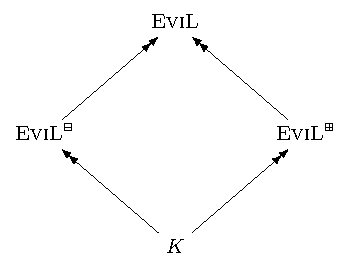
\includegraphics[]{logics/evils.pdf}
\end{center}
\caption{\textsc{EviL} conservative extensions of $K$}
\label{conservative-extensions}
\end{figure}

\begin{lemma}
	\textsc{EviL} is \textsf{PSPACE} hard 
\end{lemma}
\begin{proof}
This follows trivially from the fact that \textsc{EviL} is a conservative extension of basic modal logic, and the decision problem for basic modal logic is \textsf{PSPACE} complete.
\end{proof}

%%% Local Variables: 
%%% mode: latex
%%% TeX-master: "evil_philosophy"
%%% End: 


%\subsubsection{Completeness}\label{conservative-extension}

%\subsubsection{Conservativity, Decidability \& Complexity}


%%% Local Variables: 
%%% mode: latex
%%% TeX-master: "evil_philosophy"
%%% End: 


\section{Applications}
\subsection{Collapse}
\subsection{Epistemic Plurality}
\subsubsection{Different Kinds of Knowledge}
\subsubsection{Moore's Paradox}
\subsubsection{Fitch's Paradox}
\subsection{Intuitionistic Logic}
\subsubsection{The G\"{o}del Embedding and $\mathcal{L}^\BB(\Phi)$}
\subsubsection{Knowledge}
\subsubsection{Imagination}
\subsubsection{$ImK_\Box$}

\section{Formal Methods}\label{formal}
%\addcontentsline{toc}{subsection}{20 pgs}
%\subsection{Don't Believe in Math}
%\addcontentsline{toc}{subsubsection}{5 pgs}

\subsection{LCF Theorem Proving}
\subsection{Formalizing the \textsc{EviL} Completeness Theorem}

\section{Epilogue}
%\addcontentsline{toc}{subsection}{10 pgs}
\subsection{Comparison to Other Approaches}
\subsection{Failures}
There are several points of failure of \textsc{EviL} that I feel must be
addressed:
\begin{myRoman}
  \item \textsc{EviL} is not really a logic, because it is non-normal
    and non-compact, so it therefore any kind of reasonable algebraic
    duality is impossible \citep[for details on this, see][chapter 5]{blackburn_modal_2001} 
  \item \textsc{EviL} is not dynamic and therefore fails to conform to
    the prevailing paradigm for epistemic logics
    \item \textsc{EviL} is not completely computer verified - only the
      completeness theorem for the central axiom system for
      \textsc{EviL} has been produced; none of the many auxiliary
      results have been verified
    \item \textsc{EviL} only partly accommodates irrationality
    \item \textsc{EviL} is inhuman - the assumptions it makes for the
      nature of knowledge and \textsc{EviL} agent's cognitive
      abilities are unrealistic
\end{myRoman}

% 
% Having developed \textsc{EviL}, I feel it necessary to reengage the philosophical concerns presented in \S\ref{Human-Condition}.  \textsc{EviL} was a project to try to base an epistemic logic more on intuition and human nature, rather than the more mechanical foundation which forms the basis for mainstream epistemic logic.

\appendix
\section{Alternate Semantics}
\label{alternative}
In this section, I shall present an alternative work to the framework
proposed in \S\ref{explicit}. 
These semantics are inspired by game semantics for modal logic, 
such as those in \citet[chapter 2]{van_benthem_modal_2010}.

Consider structures of the form $\langle W, V, \beta, \iota \rangle$
consisting of:
\begin{itemizedot}
  \item A set of worlds $W$
  \item A propositional valuation function $V : \Phi \rightarrow \powerset
  W$
  \item An belief function $\beta : W \rightarrow \powerset \mathcal{L}
  (\Phi)$
   \item An imagination function $\iota : W \rightarrow \powerset W$
\end{itemizedot}
We shall call these \tmtextit{belief-imagination models}.   One can think of a
model $\Omega$ sort of like a of tuples like in \S\ref{evil-semantics}; however
in this case evidently it would have to be $\Omega \subseteq \powerset
\Phi \times \powerset \mathcal{L} (\Phi) \times \powerset \Omega$, so
apparently it would have to be a non-wellfounded set.   This is somewhat natural,
given a modal logic setting - see for instance \citep{barwise_vicious_1996} for an
elaboration on these connections.

\begin{definition}
  Define by recursion the following two truth relations:
  
  First relation:
  \begin{empt}
    \item $\Omega, w \Vdash p \Longleftrightarrow p \in V (w)$
    \item $\Omega, w \Vdash \phi \wedge \psi \Longleftrightarrow$ both $\Omega,
    w \Vdash \phi$ and $\Omega, w \Vdash \psi$
    \item $\Omega, w \Vdash \phi \vee \psi \Longleftrightarrow$ either $\Omega,
    w \Vdash \phi$ or $\Omega, w \Vdash \psi$
    \item $\Omega, w \Vdash \neg \phi \Longleftrightarrow \Omega, w \Vvdash
    \phi$
    \item $\Omega, w \Vdash \Box \phi \Longleftrightarrow \beta (w)
    \vdash^{\ast} \phi$
    
    Where $\vdash^{\ast}$ is a sequent that is closed under reflection
    and resolution:
    \begin{eqnarray*}
      \frac{\phi \in \Gamma}{\Gamma \vdash^{\ast} \phi} &  & \frac{\Gamma
      \vdash^{\ast} \neg \phi \vee \psi \ \ \  \Delta \vdash^{\ast}
      \phi}{\Gamma \cup \Delta \vdash^{\ast} \psi}
    \end{eqnarray*}
  \end{empt}
  Second relation:
  \begin{empt}
    \item $\Omega, w \Vvdash p \Longleftrightarrow p \nin V (w)$
    \item $\Omega, w \Vvdash \phi \wedge \psi \Longleftrightarrow$ either $\Omega, w \Vvdash \phi$ or $\Omega, w \Vvdash \psi$
    \item $\Omega, w \Vvdash \phi \vee \psi \Longleftrightarrow$ both $\Omega,
    w \Vvdash \phi$ and $\Omega, w \Vvdash \psi$
    \item $\Omega, w \Vvdash \neg \phi \Longleftrightarrow \Omega, w \Vdash
    \phi$
    \item $\Omega, w \Vvdash \Box \phi \Longleftrightarrow$ there is some $v
    \in \iota (w)$ such that $\Omega, v \Vvdash \phi$
  \end{empt}
\end{definition}

I feel it is necessary to motivate the intuition behind these semantics.  
Informally, I think of these two truth relations correspond to two players, whom I call the
{\tmem{logician}} and the {\tmem{philosopher}}.   The logician wields a set
beliefs given by $\beta$ and tries to compose compelling arguments, and the
philosopher employs a corpus of thought experiments given by $\iota$ to thwart
the logician's arguments.   Of course, the logician and the philosopher are
really just two aspects of a single epistemic agent I am trying to model; I
imagine epistemic agents modeled by this system to be embroiled in internal
conflict. I feel this sort of dissension between reason and imagination rages
on within us all -- it's fundamental to human nature.

These semantics are not naturally bivalent; that is it doesn't hold that
either $\Omega, w \Vdash \phi$ or $\Omega, w \Vvdash \phi$, exclusively. To
see this consider a model where $\beta (w) = \iota (w) = \varnothing$; then
evidently $\Omega, w {\nVdash} \Box p$ and $\Omega, w {\nVvdash} \Box p$.

However, bivalence has a convenient semantic characterization:

\begin{proposition}
  \label{biv1}Let $\mathbbm{M}^{\Omega} = \langle W^{\Omega}, V^{\Omega},
  R^{\Omega} \rangle$ be a model for basic modal logic model based on a
  belief/imagination model $\Omega$, where $w R^{\Omega} v \assign v \in \iota
  (w)$, and let $\Vdash_{\Box}$ be the modal truth predicate.   We have that
  $\Vdash$ and $\Vvdash$ are bivalent if and only if $\Omega, w \Vdash \phi
  \Longleftrightarrow \mathbbm{M}^{\Omega}, w \Vdash_{\Box} \phi$.
\end{proposition}

\begin{proof}
  $(\Longrightarrow)$  Assume that $\Vdash$ and $\Vvdash$ are bivalent and
  consider any $\phi \in \mathcal{L} (\Phi)$.   The proof that $\Omega, w
  \Vdash \phi$ is equivalent to $\mathbbm{M}^{\Omega}, w \Vdash_{\Box} \phi$
  proceeds by induction.   The case for proposition letters, conjunction and
  disjunction are straightforward, so we shall only consider negation and
  modality.
  
  Negation:  We have the following chain of equivalences:
  \begin{eqnarray*}
    \mathbbm{M}^{\Omega}, w \Vdash_{\Box} \neg \phi  
    \Longleftrightarrow & \mathbbm{M}^{\Omega}, w {\nVdash}_{\Box} \phi &
    \\
    \Longleftrightarrow & \Omega, w {\nVdash} \phi & (\tmop{inductive}
    \tmop{step})\\
    \Longleftrightarrow & \Omega, w \Vvdash \phi & (\tmop{bivalence})\\
    \Longleftrightarrow & \Omega, w \Vdash \neg \phi & 
  \end{eqnarray*}
  Modality: \ We have another chain of equivalences:
  \begin{eqnarray*}
    \Omega, w \Vdash \Box \phi \  \Longleftrightarrow & \Omega, w
    {\nVvdash} \Box \phi & (\tmop{bivalence})\\
    \Longleftrightarrow & \forall v \in \iota (w) .  \Omega, w {\nVvdash}
    \phi & (\tmop{definition})\\
    \Longleftrightarrow & \forall v \in \iota (w) .  \Omega, w \Vdash \phi &
    (\tmop{bivalence})\\
    \Longleftrightarrow & \forall v \in \iota (w) .\mathbbm{M}^{\Omega}, w
    \Vdash_{\Box} \phi & (\tmop{inductive} \tmop{step})\\
    \Longleftrightarrow & \forall v.w R^{\Omega} v \Longrightarrow
    \mathbbm{M}^{\Omega}, w \Vdash_{\Box} \phi & (\tmop{definition})\\
    \Longleftrightarrow & \mathbbm{M}^{\Omega}, w \Vdash_{\Box} \Box \phi & 
  \end{eqnarray*}
  This completes the induction.
  
  $(\Longleftarrow)$ \ Assume that $\Omega, w \Vdash \phi$ and
  $\mathbbm{M}^{\Omega}, w \Vdash_{\Box} \phi$ are always equivalent.   We
  have:
  \begin{eqnarray*}
    \Omega, w \Vdash \phi \  \Longleftrightarrow &
    \mathbbm{M}^{\Omega}, w \Vdash_{\Box} \phi & \\
    \Longleftrightarrow & \Omega, w {\nVdash}_{\Box} \neg \phi & \\
    \Longleftrightarrow & \Omega, w {\nVdash} \neg \phi &
    (\tmop{hypothesis})\\
    \Longleftrightarrow & \Omega, w {\nVvdash} \phi & 
  \end{eqnarray*}
\end{proof}

\begin{corollary}
  If $\Vdash$ and $\Vvdash$ are bivalent, then $\beta (w) \vdash^{\ast} \phi$
  for all $\phi \in \tmop{Th}_{\Vdash} (\Omega)$ for all $w \in W^{\Omega}$,
  where $\tmop{Th}_{\Vdash} (\Omega) =\{\phi \in \mathcal{L} (\Phi)
  \  | \  \Omega, w \Vdash \phi$ for all $w \in W^{\Omega}
  \}$.
\end{corollary}

Evidently bivalence of $\Vdash$ and $\Vvdash$ gives rise to semantics where
the agent has a proof for every proposition they believe.   Furthermore, we
can take any modal logic model $\mathbbm{M} \assign \langle W^{\mathbbm{M}},
V^{\mathbbm{M}}, R^{\mathbbm{M}} \rangle$ and define an equivalent
belief/imagination model $\Omega^{\mathbbm{M}} \assign \langle
W^{\mathbbm{M}}, V^{\mathbbm{M}}, \beta^{\mathbbm{M}}, \iota^{\mathbbm{M}}
\rangle$ where:
\begin{eqnarray}
  \beta^{\mathbbm{M}} (w) \assign & \{\phi \in \mathcal{L} (\Phi) \ 
  | \  \mathbbm{M}, w \Vdash_{\Box} \Box \phi\} &  \nonumber\\
  \iota^{\mathbbm{M}} (w) \assign & \{v \in W^{\mathbbm{M}} \  |
  \  w R^{\mathbbm{M}} v\} &  \nonumber
\end{eqnarray}
We can immediately leverage this to give the a characterization of these
semantics:

\begin{proposition}
  The basic modal logic $K$ is sound and strongly complete for bivalent
  belief/imagination models.
\end{proposition}

\begin{proof}
  Soundness is trivial given the previous lemma, strong completeness follows
  by considering the canonical model $\mathbbm{K}$ and looking at
  $\Omega^{\mathbbm{K}}$. 
\end{proof}

However, reflecting on my remarks in \S\ref{thermometers}, I think that it's wrong for agents to be able to have
everything they believe in their minds; this is about as bad as the thermometer theory of knowledge
 in my opinion.   However, this is evidently not entirely necessary. Call a belief/imagination model
\tmtextit{reasonable} if the following two constraints are satisfied:
\begin{itemizedot}
  \item $\beta (w) \vdash^{\ast} \phi$ for all $\phi \in \tmop{Th}_{\Vdash}
  (\Omega)$ for all $w \in W^{\Omega}$, where $\tmop{Th}_{\Vdash} (\Omega)
  =\{\phi \in \mathcal{L} (\Phi) \  | \  \Omega, w \Vdash
  \phi$ for all $w \in W^{\Omega} \}$
  
  \item $\tmop{Mod}^{\Omega}_{{\nVvdash}} (\beta (w)) \subseteq \iota (w)$,
  where $\tmop{Mod}^{\Omega}_{{\nVvdash}} (\beta (w)) =\{v \in W^{\Omega}
  \  | \  \Omega, v {\nVvdash} \phi$ for all $\phi \in
  \beta (w)$\}
  
  \item $\beta (w) \backslash \tmop{Th}_{\Vdash} (\Omega)$ is finite
\end{itemizedot}
Evidently, forcing these requirements suffices to force bivalence:

\begin{proposition}
  Let $\mathbbm{M}^{\Omega}$ be defined as in Prop.  \ref{biv1}.
  For any reasonable model $\Omega$ and any $w \in W^{\Omega}$, we have:
  \begin{enumerateroman}
    \item If $\mathbbm{M}^{\Omega}, w \Vdash_{\Box} \phi$ then $\Omega, w
    \Vdash \phi$
    
    \item If $\mathbbm{M}^{\Omega}, w {\nVdash}_{\Box} \phi$ then $\Omega,
    w \Vvdash \phi$
  \end{enumerateroman}  
  Hence we have $\Vdash$ and $\Vvdash$ are bivalent.
\end{proposition}

\begin{proof}
  The propositional, disjunctive and conjunctive cases are all
  straightforward; I shall focus on negation and modality.
  
  Negation: In the case of (\tmtextit{i}), we know that \
  \begin{eqnarray}
    \mathbbm{M}^{\Omega}, w \Vdash_{\Box} \neg \phi \Longleftrightarrow &
    \mathbbm{M}^{\Omega}, w {\nVdash}_{\Box} \phi &  \nonumber\\
    \Longrightarrow & \Omega, w \Vvdash \phi & \text{(by the inductive step)}
    \nonumber\\
    \Longleftrightarrow & \Omega, w \Vdash \neg \phi &  \nonumber
  \end{eqnarray}
  The proof for (\tmtextit{ii}) is similar.
  
  Modality: \ In the case of (\tmtextit{i}), assume that
  $\mathbbm{M}^{\Omega}, w \Vdash_{\Box} \Box \phi$. Using the definition of
  reasonableness and the inductive step we know for all $v \in W^{\Omega}$
  that if $\Omega, v {\nVvdash} \psi$ for all $\psi \in \beta (w)
  \backslash \tmop{Th} (\Omega)$ then $\Omega, v \Vdash \phi$.
  
  From this and the fact that $\Omega$ is reasonable we can infer that
  $\bigvee_{\psi \in \beta (w) \backslash \tmop{Th} (\Omega)} \neg \psi \vee
  \phi \in \tmop{Th}_{\Vdash} (\Omega)$.   We know further from reasonableness
  that we have $\tmop{Th}_{\Vdash} (\Omega) \subseteq \beta (w)$. So we can
  prove by induction that repeatedly applying resolution gets $\beta (w)
  \vdash^{\ast} \phi$, which just means that $\Omega, w \Vdash \Box \phi$, as
  desired.
  
  The case of (\tmtextit{ii}) follows trivially by induction.
\end{proof}

We may continue to obtain weak completeness for these semantics:

\begin{proposition}
  $\vdash_K \phi$ if and only if $\Omega, w \Vdash \phi$ for all reasonable
  models $\Omega$ and $w \in W^{\Omega}$
\end{proposition}

\begin{proof}
  Left to right follows straightforwardly, so we just need to prove right to
  left.
  
  Assume $\nvdash_K \phi$. As before, let $\mathbbm{M} = \langle
  W^{\mathbbm{M}}, V^{\mathbbm{M}}, R^{\mathbbm{M}} \rangle$ be a finite model
  and with a world $w \in W^{\mathbbm{M}}$ such that $\mathbbm{M}, w
  {\nVdash}_{\Box} \phi$.   Now consider a slightly modified model
  $\mathbbm{M}' \assign \langle W^{\mathbbm{M}}, V', R^{\mathbbm{M}} \rangle$
  where
  \[ V' (p) \assign \left\{ \begin{array}{ll}
       \{v\} & p = \rho (v)\\
       V (p) & o / w
     \end{array} \right.  \]
  A proof by induction on subformulae $\psi$ of $\phi$ verifies that
  $\mathbbm{M}, w \Vdash_{\Box} \psi$ if and only if $\mathbbm{M}', w
  \Vdash_{\Box} \psi$.
  
  So now consider $\Omega \assign \langle W^{\mathbbm{M}'}, V^{\mathbbm{M}'},
  \tau, \lambda x.R^{\mathbbm{M}'} [x] \rangle$ such that
  \[ \tau (w) \assign \tmop{Th} (\mathbbm{M}') \cup \left\{ \bigvee_{v \in
     R^{\mathbbm{M}'} [w]} \rho (v) \right\}, \]
  where $\tmop{Th} (\mathbbm{M}') \assign \{\psi \in \mathcal{L}
  (\Phi) \  | \  \mathbbm{M}', v \Vdash \psi$ for all $v
  \in W^{\mathbbm{M}'} \}$.   A proof by induction on $\psi$ shows that
  $\mathbbm{M}', w \Vdash_{\Box} \psi$, $\Omega, w \Vdash \psi$ and $\Omega, v
  {\nVvdash} \psi$ are equivalent for all $\psi \in \mathcal{L} (\Phi)$.  
  Thus we have that for all $v \in W^{\Omega}$ that $\Omega, v {\nVvdash}
  \psi$ for all $\psi \in \tmop{Th} (\mathbbm{M}')$.   Moreover, evidently $w
  R^{\mathbbm{M}'} v$ if and only if $\mathbbm{M}', v \Vdash_{\Box} \bigvee_{u
  \in R^{\mathbbm{M}'} [w]} \rho (u)$, whence we have that $w R^{\mathbbm{M}'}
  v$ if and only if $\Omega, v {\nVvdash} \chi$ for all $\chi \in \tau
  (w)$. With this we can employ induction and establish that $\mathbbm{M}', w
  \Vdash_{\Box} \psi$ if and only if $\Omega, w \models \psi$ for all $\psi
  \in \mathcal{L} (\Phi)$.   Since $\mathbbm{M}', w {\nVdash}_{\Box} \phi$,
  we have that $\Omega, w {\nmodels} \phi$.   Finally, note that in this
  model we have that $\tmop{Mod}^{\Omega}_{{\nVvdash}} (\beta (w)) =
  R^{\mathbbm{M}'} [w]$. With this and the definition of $\Omega$, we can see
  that $\Omega$ is evidently reasonable, and thus we may complete the proof.

\end{proof}

Now, while reasonable models attain the goal of modeling agents that have
proofs for the things they believe, I do not consider them adequate. These models are only reasonable in the
sense that they indeed model agents providing nontrivial proofs for their beliefs.
However, they aren't reasonable in the sense that they are simple
to reckon with.   So while the semantics provided in \S\ref{evil-semantics} requires a grammar
restriction, which might be considered inelegant, I have settled on it, rather than the formulation given above, precisely because I consider this to be less manageable.

\section{Isabelle/HOL's Logic}

\pagebreak
\addcontentsline{toc}{section}{References}
\bibliographystyle{abbrvnat}
\bibliography{zotero}
\end{document}  